
\documentclass[11pt,twoside,a4paper]{article}
\usepackage[hmargin=2cm, vmargin=2cm]{geometry}
\usepackage{microtype}
\usepackage{graphicx}
\usepackage{hyperref}
\usepackage[english]{babel}
\usepackage{setspace}
\usepackage{xcolor}
\usepackage{multicol}
\usepackage{float}
\usepackage{amsmath}
\usepackage{amsthm}
\usepackage{amssymb}
\usepackage{hyperref}
\usepackage{overpic}
\usepackage[font=small,skip=2pt]{caption}
\usepackage[
backend=biber,
style=authoryear-comp,
]{biblatex}


\newcommand{\independent}{\perp\!\!\!\!\perp} 

\addbibresource{RMbibliography.bib}
\onehalfspacing
\parindent=0pt

\begin{document}
	\title{{\LARGE Basis Choice for Scalar-on-Function Regression \\ with Applications to Near-Infrared Spectroscopy}}
	\author{Jonghun Baek, Jakob R. Juergens, Jonathan Willnow}
	\date{11.02.2022}
	\maketitle
	\vspace{1.5 cm}
	\begin{center}
		University of Bonn \\
		Research Module in Econometrics and Statistics \\
		Winter Semester 2021/2022
	\end{center}
	
	\newpage
	
	\tableofcontents
	
	\newpage
	
	\setlength{\abovedisplayskip}{0.4cm}
	\setlength{\belowdisplayskip}{0.4cm}

	\setlength{\abovedisplayshortskip}{0.2cm}
	\setlength{\belowdisplayshortskip}{0.4cm}

	\section{Introduction}
		
	Functional Data Analysis (FDA), which has its roots in the work of Ulf Grenander and Kari Karhunen, is gaining more attention as researchers from different fields collect data that is functional in nature. Although classical statistical methods can often process this data, FDA has advantages in that it allows extracting information given by properties such as the smoothness of the underlying process or its derivatives (cf. \cite{levitin_introduction_2007}).	As \cite{kokoszka_introduction_2017} describe, using methods from FDA should be considered when one variable of a given data set can be seen as smooth curves or functions.	 
	Therefore, data sets in FDA can include both realizations of scalar random variables and realizations of random functions. Examples of such curves are the absorption curves of electromagnetic radiation in the Near-infrared (NIR) spectrum by chemical samples.\footnote{For more details on Near-Infrared-Spectroscopy, refer to the \hyperref[NIR]{Section on Near-Infrared-Spectroscopy in the Appendix.}}
	
	This paper introduces Functional Linear Regression in a scalar-on-function setting. The distinct feature of this framework is that the regressor is a function, which makes a different approach to estimation necessary because the problem of estimating an unknown coefficient function is inherently infinite-dimensional. 
	We then introduce two distinct ways of translating this infinite-dimensional problem into a finite-dimensional problem that can be addressed using theory from multivariate regression: First, a so-called basis expansion of the coefficient function, and second, functional principal component regression. Both of these methods are dependent on a parameter choice called a truncation parameter for a functional basis, and this paper focuses on exploring the selection of these parameters using cross-validation.\\
	
	In Section \ref{Theory}, we introduce the necessary theoretical concepts, describe the estimation procedures, and address the theoretical importance of the truncation parameter. Section \ref{Simulation} contains a description of our Monte-Carlo Simulation, which aims to provide information on how to choose an appropriate functional basis and truncation parameter for the aforementioned methods. The application in Section \ref{Application} then uses the insights from theory and simulation to choose an appropriate basis for the estimation of Octane values of gasoline samples based on Near-Infrared absorption curves. In Section \ref{Outlook}, we give an outlook on possible extensions for this paper and describe the limitations of our approach.

	\section{Theory}\label{Theory}
	To allow for scalar-on-function regression, it is necessary to extend some concepts from multivariate regression to the realm of infinite-dimensional objects, as the statistics derived from infinite-dimensional random functions cannot be defined on a finite-dimensional space. One integral concept that must be defined is random functions as a special case of random variables. Paraphrasing a definition by \cite{bauer_wahrscheinlichkeitstheorie_2020}, a random variable $X:\Omega \rightarrow \Omega'$ is an $\mathcal{A} \text{-} \mathcal{A'} \text{-measurable}$ function, where $(\Omega, \mathcal{A}, P)$ is a probability space and $(\Omega', \mathcal{A'})$ is a measure space. 
	The typical case for a random variable realizing in $\mathbb{R}$ is $(\Omega', \mathcal{A'}) = (\mathbb{R}, \mathcal{B})$, where $\mathcal{B}$ is the canonical $\sigma$-algebra on the real numbers. As a first intuition for the concept of a random function, it is possible to imagine a similar concept where a random variable does not realize as an element of the real numbers but as a function in a function space. A formalization of this idea makes some more in-depth considerations necessary. The following theoretical introduction closely follows chapters 2.3 and 2.4 from \cite{hsing_theoretical_2015} and chapters 4.4 and 4.6 from \cite{kokoszka_introduction_2017}. 
	
	\subsection{Inner Products and Hilbert Spaces}
	The first concept we will introduce is the concept of Hilbert spaces. To do so, we start from inner product spaces but restrict our analysis to vector spaces over $\mathbb{R}$ for the sake of clarity. Let $\mathbb{V}$ be a vector space over $\mathbb{R}$.  Then, a function $\langle \cdot, \cdot \rangle : \mathbb{V} \times  \mathbb{V} \rightarrow \mathbb{R}$ is called an inner product, if $\forall v, v_1, v_2 \in \mathbb{V}$ and $a_1, a_2 \in \mathbb{R}$ the following properties hold.
	
	\begin{multicols}{2}
		\begin{enumerate}
			\item $\langle v, v \rangle \geq 0$
			\item $\langle v, v \rangle = 0$ if $v = 0$
			\item $\langle a_1 v_1 + a_2 v_2, v \rangle = a_1 \langle v_1, v \rangle + a_2 \langle v_2, v \rangle$
			\item $\langle v_1, v_2 \rangle = \langle v_2, v_1 \rangle$
		\end{enumerate}
	\end{multicols}

	A vector space with an associated inner product is called an inner product space and the inner product defines a norm and an associated distance on the vector space.
	\begin{equation}
		\lvert \lvert v \rvert \rvert = {\langle v, v \rangle}^{\frac{1}{2}} \quad \text{and} \quad 
		d(v_1, v_2) = {\langle v_2 - v_1, v_2 - v_1 \rangle}^{\frac{1}{2}}
	\end{equation}
	
	If the inner product space is complete with respect to the induced distance, it is called a Hilbert space, denoted $\mathbb{H}$ in the following. To extend the known concept of a basis in a finite dimensional space to potentially infinite Hilbert spaces, it is necessary to define the closed span of a sequence of elements of $\mathbb{H}$. Recall that the span of a set of vectors $S \subseteq \mathbb{R}^P$ is given by
	\begin{equation}
		span(S) = \left\{\sum_{i = 1}^{k} \lambda_i v_i \: \bigg\vert \: k \in \mathbb{N}, \: v_i \in S, \: \lambda_i \in \mathbb{R} \right\}
	\end{equation}
			
	The closed span $\overline{span}(S)$ of a sequence $S$ in $\mathbb{H}$ is defined as the closure of the span with respect to the distance induced by the norm and $S$ is called a basis of $\mathbb{H}$ if $\overline{span}(S) = \mathbb{H}$.	It is called an orthonormal basis if, in addition, the following properties hold. 
	
	\begin{multicols}{2}
		\begin{enumerate}
			\item $\langle v_i, v_j \rangle = 0 \quad \forall v_i, v_j \in S \quad i \neq j$
			\item $\lvert \lvert v \rvert \rvert = 1 \quad \forall v \in S$
		\end{enumerate}
	\end{multicols}

	As in the case of a Banach space, each element of a Hilbert space can be expressed in terms of a corresponding basis. This can be done using a Fourier expansion of an element $x \in \mathbb{H}$ w.r.t. a basis $S = \{s_n\}$ as follows.
	\begin{equation}
		x = \sum_{j = 1}^{\infty}{\langle x, s_j \rangle}s_j
	\end{equation}
	
	Differing from the case of Banach spaces, these representations can be limits of series. As using an infinite number of basis functions is infeasible in applied contexts, an intuitive way to approximate elements in a Hilbert space is to use a truncated series.
	\begin{equation}
		x \approx \sum_{j = 1}^{K}{\langle x, s_j \rangle}s_j
	\end{equation}
	
	\subsection{Random Functions in the Hilbert Space of Square-Integrable Functions}
	In functional data analysis, one Hilbert space of particular importance is the space of square-integrable functions on $[0,1]$. Denoted by $\mathbb{L}^2[0,1]$, this space is consists of all $\mu$-measurable functions $f(t)$ on $[0,1]$ that fulfill the following condition in which $\mu$ denotes the Lebesgue-measure.
	\begin{equation}
		\lvert \lvert f \rvert \rvert_2 = \int_{0}^{1} \lvert f \rvert^2 \mathrm{d}\mu < \infty
	\end{equation}
	
	This ensures that a random function has a finite second moment so that the variance and covariance functions can be defined. The inner product of $\mathbb{L}^2[0,1]$ is defined by Equation \ref{inner_prod}.
	\begin{equation}\label{inner_prod}
		\langle f_1, f_2 \rangle = \int_{0}^{1} f_1 f_2 \mathrm{d}\mu.
	\end{equation}
	
	$\mathbb{L}^2[0,1]$ is the function space that is most often used for theoretical considerations, but analogous constructions can be made for every closed interval of $\mathbb{R}$. 
	A random function on $\mathbb{L}^2[0,1]$ can then be defined formally as a function $X : \Omega \rightarrow \mathbb{L}^2[0,1]$ defined on a probability space $(\Omega, \mathcal{A}, P)$ where $\Omega$ is a sample space with $\sigma$-algebra $\mathcal{A}$ and a probability space $P$.
	
	\subsection{Functional Data Sets}
	If we take a random function $X(\omega)$ as defined in the previous section, then realizations $x(t)$ of $X(\omega)(t)$ are called sample curves of the random function. The presence of functional observations in a data set is what defines functional data sets. However, in reality realizations of random functions are not typically observed in their functional form. Instead, each curve is observed at a discrete and typically large set of measurements points. Consider the case of a data set containing observations $x_i(t)$ of a random function $X(\omega)$
	\begin{equation}
		x_{i}(t_{i,j}) \in \mathbb{R}, \quad i = 1,\: \dots\: ,N, \; j = 1, \: \dots \:, J_i, \; t_{i,j} \in [T_1, T_2]
	\end{equation}
	
	Each curve $x_i(t)$ exists $\forall t \in [T_1, T_2]$, but is only observed at discrete measurement points $t_{i,j}$.  These measurement points can be different for each sample curve. However, in this paper, we only consider the case where curves share their measuring points.
	To work with functional data obtained in this form using the unique capabilities of functional data analysis, it is necessary to restore its functional structure. Therefore, methods such as basis representations, which are introduced in the following parts of the Theory Section, are necessary.\\
	
	As in the finite-dimensional setting, the concept of identically distributed and independent data is important for many aspects of functional data analysis. One example of i.i.d. curves could be Near-Infrared absorption spectra of gasoline samples where each sample is produced by the same production process and can therefore be interpreted as a realization of and i.i.d. random process itself. More information about this example can be found in Appendix \ref{NIR}.
	
	\subsection{Representing a Function in terms of a Basis}\label{bases}
	As previously described, a basis of a Hilbert space can be used to express its elements using the corresponding Fourier expansion. Let therefore $\{\phi_i(t) \: \vert \: i \in \mathcal{I}\}$ be a basis used to express or approximate a realization $x(t)$ of $X(\omega)$. Then the following equation shows how a basis can be used to express a function as a weighted sum of its elements.
	\begin{equation}
		x(t) = \sum_{j \in \mathcal{I}} a_j \phi_j(t) 
	\end{equation}
	
	One very important question in this context is how the coefficients $a_j \quad j \in \mathcal{I}$ are derived given a function $x(t)$. For the purposes of this paper, this process will remain a blackbox, but detailed information on the derivation of these coefficients can be found in {\color{red} ADD CITATION!!!} \\
	Three examples of bases often used to approximate elements of $\mathbb{L}^2[0,1]$ in practice and in the later parts of this paper are explained in the following. Diagrams showing a number of basis functions from these bases are shown in Part \ref{Basis_Plots} of the Appendix.
	
	\paragraph{Monomial Basis}\label{Monomial_basis}
	A very simple idea to approximate functions in $\mathbb{L}^2[0,1]$ is to take inspiration from the well known Taylor expansion and to use monomials of increasing degree as a basis. For entire functions $f(t)$, e.g. polynomials, the exponential function or trigonometric functions, we can express the function as a potentially infinite, but converging sum of weighted monomials.
	\begin{equation}\label{Taylor_expansion}
		f(t) = \sum_{i = 1}^{\infty}a_i t^i \quad \text{where} \quad a_i = \frac{f^{(i)}(0)}{i!}
	\end{equation}
	
	However, the monomials are only a basis for the space of entire functions and not for $\mathbb{L}^2[0,1]$. But even for functions that do not fall into this category, like the logarithm, using a truncated Taylor expansion around a chosen point can lead to reasonable approximations around this specific point or even on $\mathbb{R}$ as a whole. From this idea, it is natural to use the monomials as a potential basis for approximation. \\
	As in the case of the Taylor expansion, it is not necessary to approximate a function around zero as shown above, instead one can introduce a shift parameter. This shift parameter $\alpha$ is often chosen such that the monomials are evaluated at the center point of the domain of the function.
	\begin{equation}
		\phi_{i}^{M}(t) = (t-\alpha)^i, \quad i \in \mathcal{I}
	\end{equation}

	Due to the implementation of our simulation, we will limit our paper to the case of $\alpha = 0$. However, a different choice of $\alpha$ could lead to improvements in performance of the monomial basis.
	As the monomials are not pairwise orthogonal, this basis is prone to collinearity problems, which can result in numerically unstable estimates. This restricts the number of basis functions that can be used in the estimation procedures limiting its ability to capture pronounced local peculiarities. These problems will be addressed in more detail in later parts of this paper. The limitation to a low number of monomials can additionally lead to undesirable behavior away from the point of evaluation (cf. \cite{ramsay_functional_2005}).
	\vspace{-0.2cm}
	
	\paragraph{Fourier Basis}
	In the same way the monomial basis is connected to the Taylor series, the Fourier basis corresponds to the Fourier series, which can be used to decompose a periodic function into trigonometric functions. Equation \ref{Fourier_Series} shows an example for a function with a period of 1.
	\begin{equation}\label{Fourier_Series}
		s(x) = \frac{A_0}{2} + \sum_{i = 1}^{\infty} A_i \cos(2\pi i x - \phi_i) = \frac{a_0}{2} + \sum_{i = 1}^{\infty}\left[a_i \cos(2\pi i x) + b_i \sin(2\pi i x)\right]
	\end{equation}
	
	Typically, the series is represented in the so called amplitude-phase form. This, however, is impractical for the estimation procedures shown in the later parts of this paper due to the phase shift parameter. Therefore, rewriting the series in the sine-cosine form as shown above is necessary.	
	The Fourier basis for $\mathbb{L}^2[0,1]$ is thus given by the following sequence of functions defined on $[0,1]$ directly corresponding to the terms of the sine-cosine form of the Fourier series.
	\begin{equation}
		\phi_{i}^{F}(x) = 
		\begin{cases}
			1 & \text{if} \quad i = 1\\
			\sqrt{2} \cos(\pi i x) & \text{if} \quad i \quad \text{is even} \\
			\sqrt{2} \sin(\pi (i-1)x) & \text{otherwise}
		\end{cases}
	\end{equation}

	To stay true to the original amplitude-phase form it is reasonable to restrict the number of Fourier basis functions to odd numbered values. The Fourier basis' elements exhibit a cyclical behavior which is useful to expand functions that represent a periodic or seasonal underlying process. The Fourier basis is especially suitable to expand functions with a similar curvature across the domain, generally resulting in uniformly smooth expansions. (cf. \cite{ramsay_functional_2005})
	\vspace{-0.2cm}

	\paragraph{B-spline Basis} Following chapter 3.5 from \cite{ramsay_functional_2005}, splines are defined by first dividing an interval of interest $[\tau_0, \tau_L]$ into $L$ subintervals of non-negative length divided by a non-decreasing sequence of points $(\tau_l)_{l = 1,\dots, L-1}$ called knots. On each subinterval, a spline is a polynomial of order $m = n+1$ where $n$ is its degree. If there are no multiplicities in the set of knots, the polynomials on neighboring subintervals share derivatives up to order $m-2$ at the boundary knot $\tau_l$. A typical case that is often used in practice is an equidistant grid of knots. In some settings, however, it can be sensible to place multiple knots at the same value to replicate specific properties of the data structure allowing for a reduced number of matching derivatives at the corresponding knots. For the purposes of this paper, we will focus on the case of equidistant knots without multiplicity at inner knots.\\
	
	B-splines are a specific system of spline functions developed by \cite{de_boor_practical_1978} and are defined by a recursive procedure. Let $\phi_{l,m}^{BS}(x) \quad l \in \{1,\dots,L-1\}$ be a B-spline of order $m$ for an interval $[\tau_0, \tau_L]$ and inner knots $\{\tau_l \: \vert \: l = 1,\dots, L-1\}$, then it is defined by the Cox-de Boor recursion formula as follows. 
	\begin{equation}
		\begin{split}
			\phi_{l,0}^{BS}(x) = &
			\begin{cases}
				1 & \text{if} \quad x \in \left[\tau_l, \tau_{l+1}\right)\\
				0 & \text{otherwise}
			\end{cases}\\ \\
			\phi_{l,m}^{BS}(x) = &\frac{x - \tau_l}{\tau_{l+m} - \tau_l} \phi_{l,m-1}^{BS}(x) + \frac{\tau_{l+m+1} - x}{\tau_{l+m+1} - \tau_{l+1}} \phi_{l+1,m-1}^{BS}(x)
		\end{split}
	\end{equation}
	
	As this equation references knots that are not defined by the original vector of knots, implementations of this algorithm typically repeat the knots at the boundaries of the interval, $\tau_0$ and $\tau_L$ an additional $m$ times. This padding of the knot vector then allows to calculate every object that is needed for the definition of the basis over the original set of knots.\\
	
	This, however, does not lead to a basis of $\mathbb{L}^2[0,1]$ as the closed span of this finite sequence of functions is not equal to $\mathbb{L}^2[0,1]$. To focus on specific approximation errors in the later parts of this paper, we will, however, assume that a B-spline basis representation of a function in $\mathbb{L}^2[0,1]$ will serve as a sufficient approximation for an appropriately chosen number of B-spline basis functions. 
	
	As the B-spline basis does not have infinitely many elements as the full monomial or Fourier bases do, it is slightly misleading to speak of truncating the B-spline basis at a truncation parameter $L$ in later parts of this paper. For the sake of keeping the notation reasonably concise, we will still keep this notation. However, by convention, truncating a B-spline basis at truncation parameter $L$ shall mean using a B-spline basis consisting of $L$ functions from this point on.
	
	\subsection{Approximation and Smoothing via Basis Truncation}
	Realized curves from a data set can be expressed in terms of a chosen functional basis. For this expansion, it is  possible to use a complete basis of $\mathbb{L}^2[0,1]$. In many cases this is not a desirable approach as this expansion can introduce high amounts of variance or even lead to the approximation of noise in the sample curves, the latter being a typical case of overfitting. To combat this problem, smoothing methods such as, for example, acceleration penalties are employed to enforce a degree of smoothness in the analyzed curves. On the other hand, important information on the curves could be missed by smoothing the data too much by giving too much weight to a chosen penalty term leading to oversmoothing and loss of valuable information. This is a typical occurence of the Bias-Variance tradeoff.\\
	
	A different approach that is atypical in practice, is to enforce smoothing by limiting the number of basis functions in the approximation of the functional objects. Here, the parameter of choice is not a weighting term for the penalty, but the number of basis functions. Exploring this alternative smoothing method in two different estimation procedures is the main focus of this paper. A truncated basis expansion as described above is given in Equation \ref{basis_exp}.
	\begin{equation}\label{basis_exp}
		X(\omega_0) = x(t) = \sum_{j \in \mathcal{I}} A_j(\omega_0) \phi_j(t) = \sum_{j = 1}^{L} A_j(\omega_0) \phi_j(t) + \delta(t) \approx \sum_{j = 1}^{L} A_j(\omega_0) \phi_j(t)
	\end{equation}

	where $\delta(t)$ is the truncation error and $L \leq \max\limits_{j \in \mathcal{I}}(j)$ for all $L \in \mathcal{I}$.  In later parts, this approximation error is explicitly denoted in the derivation and then omitted for the final approximations. $L$ can be chosen subjectively, but also through applying data-driven methods such as Cross-Validation. Figure \ref{Different_Expansions} shows the effect of choosing different numbers of basis functions for one observation of the Near-Infrared Spectroscopy data set which is used in the later parts of this paper and exemplifies the tradeoffs that are at the core of the truncation parameter choice.
			
	\begin{figure}[H]
		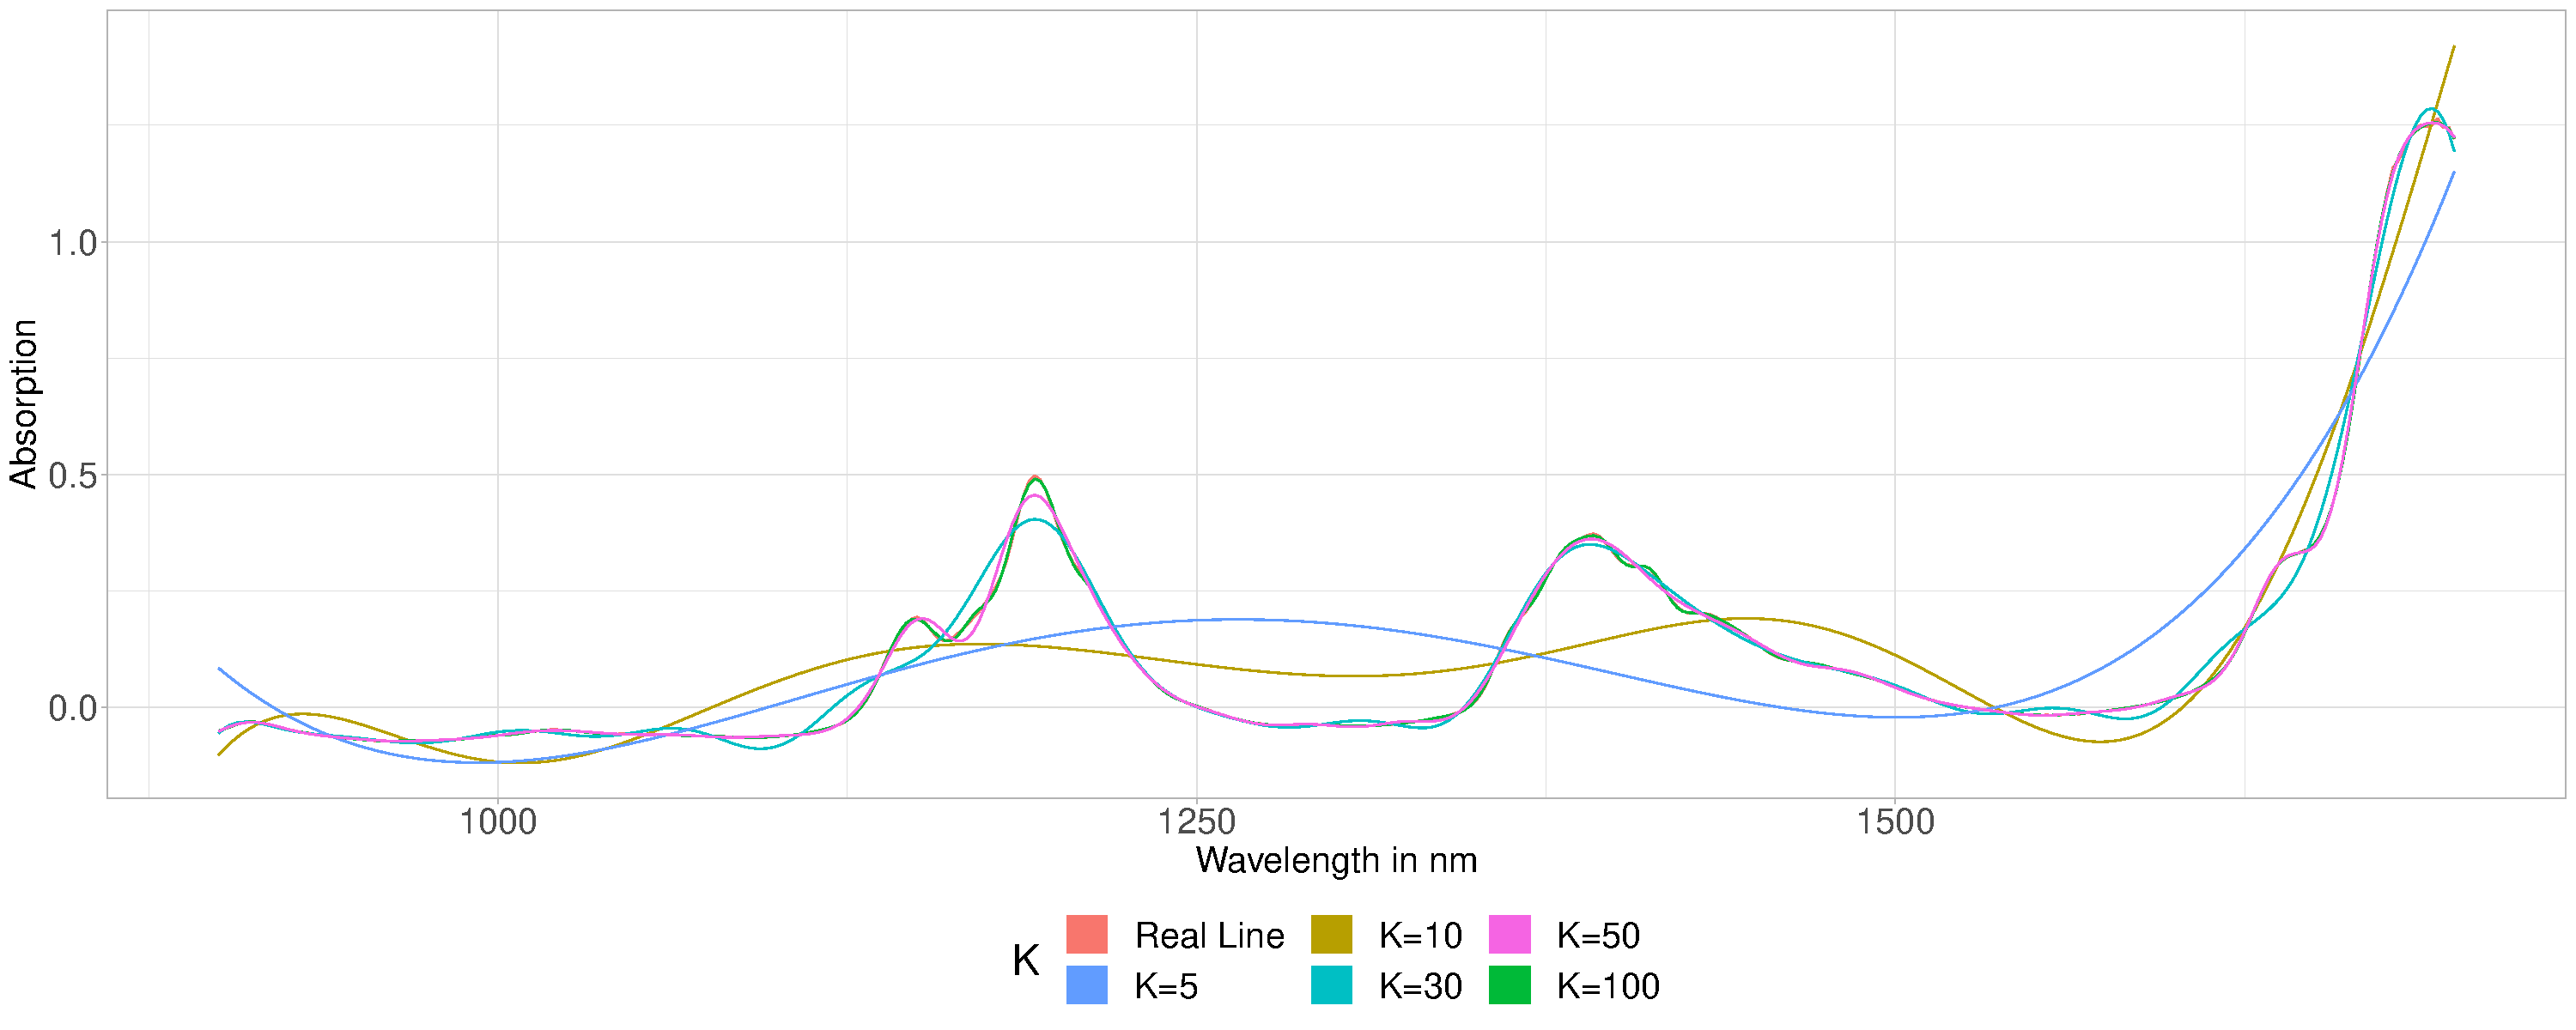
\includegraphics[width=\textwidth]{../Graphics/basis_expansions.pdf}
		\caption{B-spline Approximations of NIR Absorption Spectra with different Basis Truncation Parameters}
		\label{Different_Expansions}
	\end{figure}
	
	\subsection{Karhunen-Lo\'{e}ve Expansion and Empirical Eigenbases}\hypertarget{KL}{}
	Given a random function $X: \Omega \mapsto \mathbb{L}^2[0,1]$, it is possible to represent its realizations in terms of the stochastic process. To do so, we define the mean and covariance functions of $X(\omega)$.
	\begin{equation}\label{MeanFunction}
		\mu(t) = \mathbb{E}\left[ X(\omega)(t) \right]
	\end{equation}
	\begin{equation}\label{CovarianceFunction}
		c(t,s) = \mathbb{E}\big[ \left( X(\omega)(t) - \mu(t) \right) \left( X(\omega)(s) - \mu(s) \right) \big]
	\end{equation}

	where the $c: [0,1] \times [0,1] \rightarrow \mathbb{R}$ are Hilbert-Schmidt Kernels and $K$ is a corresponding Hilbert-Schmidt integral operator\footnote{Definitions of Hilbert-Schmidt Kernel and Integral Operator are provided in Appendix \ref{def_HS}.} $K : \nu \rightarrow K \nu$ for $\nu \in \mathbb{L}^{2}[0,1]$ defined by
	\begin{equation}\label{HSKernal}
		[K \nu](t) = \int_{0}^{1}c(t,s) \nu(s)ds = \lambda \nu(t)
	\end{equation}

	Then, the operator $K$ has orthonormal basis functions $\nu^{m} \in \mathbb{L}^{2}[0,1]$ each corresponding to an Eigenvalue $\lambda^{m}$ since it is a positive compact self-adjoint operator (cf. \cite{alexanderian_KLexpansion_2015}).
	Theoretical considerations lead to the result that $X$ can be represented in the following form, called its Karhunen-Lo\'{e}ve expansion.\footnote{Proofs for these theorems are provided in Appendix \ref{Proof1} and \ref{Proof2}.} 
	\begin{equation}\label{KarhunenLoeve}
		X(\omega)(t) = \mu(t) + \sum_{m = 1}^{\infty} \xi^m(\omega) \nu^m(t), \quad \xi^m(\omega) =  \int_{0}^{1} \left(X(\omega)(s) - \mu(s)\right) \nu^m(s) \mathrm{d}s
	\end{equation}

	where the $\nu^m$ are defined by the countable set of solutions $\{(\lambda^m, \nu^m) \: \vert \: m \in \mathbb{N}\}$ of Equation \ref{HSKernal} and the random variables $\xi^{m}(\omega)$ satisfy the following properties.
	\begin{multicols}{2}
		\begin{enumerate}
			\item $\mathbb{E}\left[\xi^m(\omega)\right] = 0$
			\item $Cov\left(\xi^m(\omega), \xi^n(\omega)\right) = 0$ if $m \neq n$
			\item $Var\left(\xi^m(\omega)\right) = \lambda^m$
		\end{enumerate}
	\end{multicols}

	As in the well known setting of principal component analysis, the Eigenvalues correspond to the variance in the random function that is explained by the corresponding Eigenfunction. 
	Therefore, ordering the the Eigenfunctions according to their their corresponding Eigenvalues $\lambda^{1} \geq \lambda^{2} \geq \dots \geq 0$ is useful for approximation purposes. Due to this property a functional observation can often be approximated well by using a limited number of the Eigenfunctions of its generating random process. Moreover, our data generating process for the simulation study is based on this property as explained in Section \ref{similar_curves}.\\
	
	In the scalar setting, a similar consideration leads to the concept of principal components, which can be extended to the functional setting. Let $\{x_1(t), \dots, x_n(t)\}$ be a set of i.i.d. realizations generated by a random function $X(\omega) \mapsto \mathbb{L}^2[0,1]$.
	Define the following sample analogs for the mean and covariance functions.
	\begin{equation}
		\hat{\mu}(t) = \frac{1}{N}\sum_{i = 1}^{N}x_i(t)
	\end{equation}
	\begin{equation}
		\hat{c}(t,s) = \frac{1}{N} \sum_{i = 1}^{N} \left(x_i(t) - \hat{\mu}(t)\right) \left(x_i(s) - \hat{\mu}(s)\right)
	\end{equation}
	
	With these it is possible to derive a set of sample analogs $\{(\hat{\lambda}^m, \hat{\nu}^m) \: \vert \: m = 1,\: \dots\:, N-1\}$ for $\{(\lambda^m, \nu^m) \: \vert \: m = 1, 2, \:\dots\}$ as the solutions of the following equation. 
	\begin{equation}
		\int_{0}^{1}\hat{c}(t,s)\hat{\nu}(s) \mathrm{d}s = \hat{\lambda} \hat{\nu}(t)
	\end{equation}

	
	In the following, we will call the $\hat{\nu}^m(s)$ functional principal components to distinguish the sample analogs from the theoretical Eigenfunctions $\nu^m(s)$. As in the case of ordinary principal components, the number of functional principal components corresponding to non-zero Eigenvalues is limited (cf. chapter 8.2.3 \cite{ramsay_functional_2005}). As each curve is infinite dimensional, there is no upper limit to this number due to the dimensionality. However, the number of curves still imposes an upper limit of $N-1$ non-zero Eigenvalues, where $N$ is the number of curves in the data set.
	These sample analogs naturally lead to the following representation of each sample curve $x_i(t)$.
	\begin{equation}
		x_i(t) = \hat{\mu}(t) + \sum_{j = 1}^{N-1} \hat{\xi}_{i}^{m} \hat{\nu}^{m}(t)
	\end{equation}

	where the $\hat{\xi}_{i}^m$ are derived as 
	\begin{equation}
		\hat{\xi}_i^m(\omega) = \langle x_i - \hat{\mu}, \hat{\nu}^m\rangle = \int_{0}^{1} \left(x_i(s) - \hat{\mu}(s)\right) \hat{\nu}^m(s) \mathrm{d}s
	\end{equation}
	
	In reality, these calculations are often implemented using basis representations of both the functional principal components $\hat{\nu}^m$ and the observations $x_i(t)$ leading to the following representation. For the sake of clarity, the following equation assumes that the bases used for the expansion of both the observations and the coefficient function are true bases of $\mathbb{L}^2[0,1]$ and can therefore be used to express the corresponding objects exactly.
	\begin{equation}\label{FPCA_basis_expansion}
		\begin{split}
			\hat{\xi}_{i}^m & = \int_{0}^{1} {\color{red}\left( x_i(s) - \hat{\mu}(s)\right)} {\color{blue}\hat{\nu}^m(s)} \mathrm{d}s
			= \int_{0}^{1} {\color{red}\left(\sum_{j \in \mathcal{I}} a_{i,j} \phi_j(s)\right)} {\color{blue}\left(\sum_{k \in \mathcal{L}} d_{k}^m \psi_{k}(s)\right)} \mathrm{d}s \\
			& = \int_{0}^{1} {\color{red}\left(\sum_{j = 1}^{J} a_{i,j} \phi_j(s) + \delta_i^J(s)\right)} {\color{blue}\left(\sum_{k = 1}^{K} d_{k}^m \psi_{k}(s) + \delta_{\nu}^{m,K}(s)\right)} \mathrm{d}s \\
			& = \sum_{j = 1}^{J} \left[a_{i,j}\sum_{k = 1}^{K} d_{k}^m \int_{0}^{1} \phi_j(s) \psi_{k}(s)\mathrm{d}s \right] +  \sum_{k = 1}^{K} d_{k}^m \int_{0}^{1} \delta_i^J(s) \psi_{k}(s) \mathrm{d}s \\
			& \quad + \sum_{j = 1}^{J} a_{i,j} \int_{0}^{1}\phi_j(s) \delta_{\nu}^{m,K}(s) \mathrm{d}s + \int_{0}^{1} \delta_i^J(s) \delta_{\nu}^{m,K}(s) \mathrm{d}s
		\end{split}
	\end{equation}
	
	In practice, a typical choice is to use the same basis $\left(\phi_j(t)\right)_{j \in \mathcal{I}}$ and the same truncation parameter $L$ for the basis expansion of the demeaned observations $\left(x_i(t) - \hat{\mu}(t)\right)$ and the functional principal components $\hat{\nu}^m$. This leads to the following simplification of Equation \ref{FPCA_basis_expansion}.
	\begin{equation}\label{score_approx}
		\begin{split}
			\hat{\xi}_{i}^m &= \sum_{j = 1}^{L} \left[a_{i,j}\sum_{k = 1}^{L} d_{k}^m \int_{0}^{1} \phi_j(s) \phi_{k}(s)\mathrm{d}s \right] +  \sum_{k = 1}^{L} d_{k}^m \int_{0}^{1} \delta_i^L(s) \phi_{k}(s) \mathrm{d}s \\
			& \quad + \sum_{j = 1}^{L} a_{i,j} \int_{0}^{1}\phi_j(s) \delta_{\beta}^L(s) \mathrm{d}s + \int_{0}^{1} \delta_i^L(s) \delta_{\beta}^L(s) \mathrm{d}s
		\end{split}
	\end{equation}

	And we can define the following objects:
		\begin{align}
			\tilde{\xi}^{m,L}_{i} & := \sum_{j = 1}^{L} \left[a_{i,j}\sum_{k = 1}^{L} b_{k}^m \int_{0}^{1} \phi_j(s) \phi_{k}(s)\mathrm{d}s \right] 
			& \delta_{\xi, i}^L & := \hat{\xi}_{i}^m - \tilde{\xi}^{m,L}_{i} \\
			\tilde{\nu}^{m,L}(t) & := \sum_{k = 1}^{L} d_{k}^m \phi_{k}(t) 
			& \delta_{\nu}^{m, L}(t) & := \hat{\nu}^m(t) - \tilde{\nu}^{m,L}(t)
		\end{align}	
	
	This method of deriving or approximating the Eigenfunctions and scores from a data set is introduced in \cite{ramsay_functional_2005} (chapter 8.4.2) and implemented in the R-package fda. The following considerations and results of the simulation study might therefore serve as information about the performance of this method in a scenario where a limited number of basis functions is provided to the method instead of using more conventional smoothing approaches.
	
	\subsection{Scalar-on-Function Regression}\label{Scalar_on_function_regression}
	In the simple scalar setting, one of the most important tools in econometrics is linear regression. Its goal is twofold: to gain information about the dependency between variables, but also to allow for prediction. To motivate the jump from multivariate regression to scalar-on-function regression, assume a data generating process as follows.
	\begin{equation}
		Y = X\beta + \epsilon
	\end{equation}
	
	Here, $Y$ is the vector of response variables, $X$ is the matrix containing the corresponding regressors in its columns and $\beta = (\beta_0, \beta_1, \: \dots, \beta_p)'$ is the vector containing the unknown coefficients.
	In this finite dimensional setting one important question is how to estimate the unknown coefficients $\beta$. The most well known estimator in all of econometrics, the Ordinary Least Squares (OLS) estimator, fulfills this purpose under a set of assumptions.
	\begin{equation}
		\hat{\beta}_{OLS} = (X'X)^{-1}X'Y
	\end{equation}
	
	The concept of linear regression can be extended to a setting of functional data, where a scalar response variable is assumed to be dependent on a functional regressor. 
	Even though integrating over the product of an observation with the coefficient function is not the only functional that can be used to create a data generating process involving functional observations, it is the most typical as it naturally extends the intuition from multiple linear regression to the realm of infinite-dimensional objects. Therefore, we will always assume a data generating process as follows in this paper.
	\begin{equation}\label{DGP}
		Y(\omega) = \alpha + \int_{0}^{1} \beta(s)X(\omega)(s) \mathrm{d}s + \epsilon(\omega)
	\end{equation}
	
	Similar to the finite-dimensional setting, an interesting question is how to estimate the unknown coefficient function $\beta(t)$ given a data set containing realizations of a random function and associated scalar response variables. However, a simple extension of the OLS estimator to allow for infinite-dimensional objects is not possible. Therefore, other options have to be considered, two of which will be explained in the following.
	
	\subsubsection{Estimation using Basis-Representation}\label{basis_exp_transf}
	The most common way to make this problem tractable is via a basis representation of $\beta(t)$. Therefore, let $\{\phi_i(t) \: \vert \: i \in \mathcal{I}\}$ be a basis of $\mathbb{L}^2[0,1]$ and represent $\beta(t)$ in terms of this basis.
	\begin{equation}
		\beta(t) = \sum_{j \in \mathcal{I}} b_j \phi_j(t)
	\end{equation}
	
	This enables us to write equation \ref{DGP} using this representation to obtain a formulation as a sum of scalar random variables $Z_j(\omega)$.
	\begin{equation}
		\begin{split}
			Y(\omega) & = \alpha + \int_{0}^{1} {\color{blue}\beta(s)} X(\omega)(s)\mathrm{d}s + \epsilon(\omega)
			= \alpha + \int_{0}^{1}\left[{\color{blue}\left(\sum_{j \in \mathcal{I}} b_j \phi_j(s)\right)} X(\omega)(s) \right]\mathrm{d}s + \epsilon(\omega) \\
			& = \alpha + \sum_{j \in \mathcal{I}} \left[b_j \textcolor{red}{\int_{0}^{1} X(\omega)(s) \phi_j(s)\mathrm{d}s}\right] + \epsilon(\omega)
		      = \alpha + \sum_{j \in \mathcal{I}} b_j \textcolor{red}{Z_j(\omega)} + \epsilon(\omega)
		\end{split}
	\end{equation}
	
	This representation translates the original problem of regressing a scalar on a continuously observed function to a problem where a scalar is regressed on what is possibly a countably infinite sequence of regressors. Using a truncation of the basis at some parameter $J$ can be used to make this problem tractable if we assume that the approximation error created by this truncation is small.
	\begin{equation}
		\begin{split}
			Y(\omega) & = \alpha + \int_{0}^{1}\left[{\color{blue}\left(\sum_{j = 1}^{J} b_j \phi_j(s) + \delta_{\beta}^{J}(s)\right)} X(\omega)(s) \right]\mathrm{d}s + \epsilon(\omega) \\
			& = \alpha + \sum_{j = 1}^{J} b_j \int_{0}^{1} \phi_j(s) X(\omega)(s) \mathrm{d}s +  \int_{0}^{1} \delta_{\beta}^{J}(s) X(\omega)(s) \mathrm{d}s + \epsilon(\omega)
		\end{split}
	\end{equation}

	In practice it is common to not only express the coefficient function in terms of a basis but also the observations. Therefore two bases ($\left(\phi_j(t)\right)_{j \in \mathcal{I}}$ and $\left(\psi_k(t)\right)_{k \in \mathcal{L}}$) and two corresponding truncation parameters ($J$ and $K$) can be chosen. This leads to the following representation.
	\begin{equation}
		\begin{split}
			Y(\omega) & = \alpha + \int_{0}^{1} {\color{blue}\beta(s)} {\color{red}X(\omega)(s)}\mathrm{d}s + \epsilon(\omega)
			 = \alpha + \int_{0}^{1}\left[{\color{blue}\left(\sum_{j \in \mathcal{I}} b_j  \phi_j(s)\right)} {\color{red}\left(\sum_{k \in \mathcal{L}} a_k(\omega)  \psi_k(s)\right)} \right]\mathrm{d}s + \epsilon(\omega) \\
			& = \alpha + \int_{0}^{1}\left[{\color{blue}\left(\sum_{j = 1}^{J} b_j  \phi_j(s) + \delta_{\beta}^{J}(s)\right)} {\color{red}\left(\sum_{k = 1}^K a_k(\omega)  \psi_k(s) + \delta_{X}^{K}(\omega)(s)\right)} \right]\mathrm{d}s + \epsilon(\omega)\\
			& = \alpha + \sum_{j = 1}^J b_j \left[\sum_{k = 1}^K a_k(\omega) \int_{0}^{1} \phi_j(s) \psi_k(s) \mathrm{d}s\right] + \sum_{j = 1}^{J} b_j  \int_{0}^{1} \phi_j(s) \delta_{X}^{K}(\omega)(s) \mathrm{d}s\\
			& \quad \quad + \sum_{k = 1}^{K} a_k(\omega)  \int_{0}^{1} \delta_{\beta}^{J}(s)\phi_j(s) \mathrm{d}s + \epsilon(\omega) + \int_{0}^{1}  \delta_{\beta}^{J}(s) \delta_{X}^{K}(\omega)(s) \mathrm{d}s
		\end{split}
	\end{equation}

	A typical choice in this scenario is to use the same functional basis $\left(\phi_j(t)\right)_{j \in \mathcal{I}}$ and the same truncation parameter $L$ for both the coefficient function and the approximation of the observations. Using the following notation 
	\begin{equation}
			\tilde{Z}_j(\omega) = \sum_{k = 1}^{L} \left[a_k(\omega) \int_{0}^{1} \phi_j(s) \phi_k(s) \mathrm{d}s \right] \quad j = 1, \dots, L
	\end{equation}

	this leads to a considerable simplification of Equation \ref{basis_exp_transf}.
	\begin{equation}\label{simplified_model_basis_equation}
		\begin{split}
			Y(\omega) &= \alpha + \sum_{j = 1}^{L} b_j \tilde{Z}_j(\omega) + \sum_{j = 1}^{L} b_j  \int_{0}^{1} \phi_j(s) \delta_{X}^{L}(\omega)(s) \mathrm{d}s\\
			& \quad \quad + \sum_{k = 1}^{L} a_k  \int_{0}^{1} \delta_{\beta}^{L}(s)\phi_j(s) \mathrm{d}s + \epsilon(\omega) + \int_{0}^{1}  \delta_{\beta}^{L}(s) \delta_{X}^{L}(\omega)(s) \mathrm{d}s + \epsilon(\omega)\\
			& \approx \alpha + \sum_{j = 1}^{J} b_j \tilde{Z}_j(\omega) + \epsilon(\omega)
		\end{split}
	\end{equation}

	A model in the form of Equation \ref{simplified_model_basis_equation} naturally lends itself to be estimated using theory from multivariate linear regression. Define therefore the following objects
	\begin{equation}\label{regressor_mat_1}
		Y = \begin{pmatrix}
			y_1 \\ \vdots \\ y_n
		\end{pmatrix}, \quad
		Z = \begin{pmatrix}
			1 & \tilde{Z}_{1,1} & \dots & \tilde{Z}_{1,J} \\
			\vdots & \vdots & \ddots & \vdots \\
			1 & \tilde{Z}_{N,1} & \dots & \tilde{Z}_{N,J}
		\end{pmatrix}
	\end{equation}
	
	Then an OLS estimator can be calculated in the usual way to obtain an estimate for the values of $\alpha$ and $b_j$ and an estimate of the coefficient function can be derived accordingly.
	\begin{equation}
		b^L = \left(Z'Z\right)^{-1}Z'Y \in \mathbb{R}^{L+1} \quad \hat{\alpha} = b_{1}^{L} \quad \hat{\beta}^L(t) = \sum_{j = 1}^{J} b_{j+1}^L \phi_j(t)
	\end{equation}

	The performance of this estimation procedure depends in part on the quality of the approximation in Equation \ref{simplified_model_basis_equation}. Therefore, it is interesting to think about when the approximation error is small... {\color{red}Continue Here Jakob!!!}
	
	\subsubsection{Estimation using Functional Principal Components}\label{fpc_exp_transf}
	
	Using the Karhunen-Lo\'{e}ve Expansion to represent $X(\omega)$, it is also possible to express the data generating process in terms of the Eigenfunctions of $X(\omega)(t)$.
	\begin{equation}
		\begin{split}
			Y(\omega) &= \alpha + \int_{0}^{1} {\color{red}X(\omega)(s)} \beta(s) \mathrm{d}s + \epsilon(\omega)
			= \alpha + \int_{0}^{1} {\color{red}\left(\mu(s) + \sum_{m = 1}^{\infty} \xi^m(\omega) \nu^m(s)\right)} \beta(s) \mathrm{d}s + \epsilon(\omega)\\
			&= {\color{teal}\alpha + \int_{0}^{1} \mu(s) \beta(s) \mathrm{d}s} + \sum_{m = 1}^{\infty} \xi^m(\omega) {\color{violet}\int_{0}^{1} \nu^m(s) \beta(s) \mathrm{d}s} + \epsilon(\omega)
			= {\color{teal}\bar{\alpha}} + \sum_{m = 1}^{\infty} \xi^m(\omega) {\color{violet}\beta^m} + \epsilon(\omega)
		\end{split}
	\end{equation}

	As these theoretical Eigenfunctions and Eigenvalues are typically unknown, the corresponding equation in sample analogs is more interesting as a representation of an observation.
	\begin{equation}
		\begin{split}
			y_i &= \alpha + \int_{0}^{1} {\color{red}x_i(s)} \beta(s) \mathrm{d}s + \epsilon_i
			= \alpha + \int_{0}^{1} {\color{red}\left(\hat{\mu}(s) + \sum_{m = 1}^{N-1} \hat{\xi}^m_i \hat{\nu}^m(s)\right)} \beta(s) \mathrm{d}s + \epsilon_i\\
			&= {\color{teal}\alpha + \int_{0}^{1} \hat{\mu}(s) \beta(s) \mathrm{d}s} + \sum_{m = 1}^{N-1} \hat{\xi}^m_i {\color{violet}\int_{0}^{1} \hat{\nu}^m(s) \beta(s) \mathrm{d}s} + \epsilon_i
			= {\color{teal}\bar{\alpha}} + \sum_{m = 1}^{N-1} \hat{\xi}^m_i {\color{violet}\hat{\beta}^m} + \epsilon_i
		\end{split}
	\end{equation}
	
	This, however, is a simplification for the purposes of real-world estimation as in most implementations, the coefficient function and the principal components are also expressed or derived in terms of a basis that can be chosen freely. Introducing both concepts one step at a time leads to the following complication if we first introduce an expansion of the coefficient function.
	\begin{equation}
		\begin{split}
			y_i &= \alpha + \int_{0}^{1} {\color{red}x_i(s)} {\color{blue}\beta(s)} \mathrm{d}s + \epsilon_i
			= \alpha + \int_{0}^{1} {\color{red}\left(\hat{\mu}(s) + \sum_{m = 1}^{N-1} \hat{\xi}^{m}_i \hat{\nu}^{m}(s)\right)} {\color{blue}\left(\sum_{j \in \mathcal{I}} b_j \phi_j(s)\right)} \mathrm{d}s + \epsilon_i\\
			&= \alpha + \int_{0}^{1} \left[ \sum_{j \in \mathcal{I}} b_j \phi_j(s) \hat{\mu}(s) + \sum_{m = 1}^{N-1} \left[ \hat{\xi}^m_i \sum_{j \in \mathcal{I}} b_j \hat{\nu}^m(s) \phi_j(s) \right] \right] \mathrm{d}s + \epsilon_i \\
			&= \alpha + \sum_{j \in \mathcal{I}} b_j \int_{0}^{1} \phi_j(s) \hat{\mu}(s) \mathrm{d}s + \sum_{m = 1}^{N-1} \left[ \hat{\xi}^m_i \sum_{j \in \mathcal{I}} b_j \int_{0}^{1}\hat{\nu}^m(s) \phi_j(s) \mathrm{d}s \right] + \epsilon_i
		\end{split}
	\end{equation}

	Truncating the basis used for expansion of the coefficient function already introduces an approximation error.
	\begin{equation}\label{fpcr_reg_both_expansions}
		\begin{split}
			y_i &= \alpha + \int_{0}^{1} \left(\hat{\mu}(s) + \sum_{m = 1}^{N-1} \hat{\xi}^{m}_i \hat{\nu}^{m}(s)\right) {\color{blue}\left(\sum_{j = 1}^{J} b_j \phi_j(s) + \delta_{\beta}^{J}(s)\right)} \mathrm{d}s + \epsilon_i\\
			&= \alpha + \sum_{j = 1}^{J} b_j \int_{0}^{1} \phi_j(s) \hat{\mu}(s) \mathrm{d}s + \int_{0}^{1} \delta_{\beta}^{J}(s) \hat{\mu}(s) \mathrm{d}s + \sum_{m = 1}^{N-1} \left[ \hat{\xi}^m_i \sum_{j = 1}^{J} b_j \int_{0}^{1}\hat{\nu}^m(s) \phi_j(s) \mathrm{d}s \right] \\
			& \quad \quad + \sum_{m = 1}^{N-1} \left[ \hat{\xi}^m_i \int_{0}^{1}\hat{\nu}^m(s) \delta_{\beta}^{J}(s) \mathrm{d}s \right] + \epsilon_i
		\end{split}
	\end{equation}

	If we additionally derive and approximate the principal components and corresponding scores using a truncated basis representation as in Equation \ref{score_approx} we obtain the following. To not complicate things more than necessary, the following equation assumes that the same basis $\left(\phi_j(t)\right)_{j \in \mathcal{I}}$ was used in the derivation of the principal components and the expansion of the coefficient function. Additionally, the following approximation truncates the basis for the expansion of the coefficient function at the same parameter $L$ that was used for the approximation of the principal components and scores.
	
	For convenience, define the following notation:
	\begin{equation}
		\tilde{\alpha}^L = \alpha + \sum_{j = 1}^{L} b_j \int_{0}^{1} \phi_j(s) \hat{\mu}(s) \mathrm{d}s + \int_{0}^{1} \delta_{\beta}^{L}(s) \hat{\mu}(s) \mathrm{d}s
	\end{equation}
	
	Then Equation \ref{fpcr_reg_both_expansions} can be expressed as follows.
	\begin{equation}
		\begin{split}
			y_i & = \tilde{\alpha}^L
			+ \sum_{m = 1}^{N-1} \left[ \left(\tilde{\xi}^{m,L}_{i} + \delta_{\xi, i}^{m, L} \right) \sum_{j = 1}^{L} b_j \int_{0}^{1} \left(\tilde{\nu}^{m,L}(s) + \delta_{\nu}^{m,L}(s) \right) \phi_j(s) \mathrm{d}s \right] 
			+ \epsilon_i \\
			& = \tilde{\alpha}^L
			+ \sum_{m = 1}^{N-1} \left[ \tilde{\xi}^{m,L}_{i} \sum_{j = 1}^{L} b_j \int_{0}^{1} \tilde{\nu}^{m,L}(s) \phi_j(s) \mathrm{d}s \right] 
			+ \sum_{m = 1}^{N-1} \left[ \tilde{\xi}^{m,L}_{i} \sum_{j = 1}^{L} b_j \int_{0}^{1} \delta_{\nu}^{m,L}(s) \phi_j(s) \mathrm{d}s \right] \\
			& \quad \quad + \sum_{m = 1}^{N-1} \left[ \delta_{\xi, i}^{m, L} \sum_{j = 1}^{L} b_j \int_{0}^{1} \tilde{\nu}^{m,L}(s) \phi_j(s) \mathrm{d}s \right] 
			+ \sum_{m = 1}^{N-1} \left[ \delta_{\xi, i}^{m, L} \sum_{j = 1}^{L} b_j \int_{0}^{1} \delta_{\nu}^{m,L}(s) \phi_j(s) \mathrm{d}s \right]
			+ \epsilon_i \\
			& \approx \tilde{\alpha}^L
			+ \sum_{m = 1}^{N-1} \left[ \tilde{\xi}^{m,L}_{i} \sum_{j = 1}^{L} b_j \int_{0}^{1} \tilde{\nu}^{m,L}(s) \phi_j(s) \mathrm{d}s \right] + \epsilon_i
		\end{split}
	\end{equation}

	The parameter $M \in \{1,\: \dots \:, N-1\}$ corresponds to the chosen number of principal components and therefore constitutes another choice in the approximation. Using only $M$ functional principal components leads to the following approximation.
	\begin{equation}
		y_i \approx \tilde{\alpha}^L
		+ \sum_{m = 1}^{M} \left[ \tilde{\xi}^{m,L}_{i} {\color{red}\sum_{j = 1}^{L} b_j \int_{0}^{1} \tilde{\nu}^{m,L}(s) \phi_j(s) \mathrm{d}s} \right] + \epsilon_i 
		= \tilde{\alpha}^L
		+ \sum_{m = 1}^{M} \tilde{\xi}^{m,L}_{i} {\color{red}\bar{b}^{m,L}} + \epsilon_i
	\end{equation}
	

	As in the previous section, this equation lends itself for estimation with OLS and we can define the following objects.
	\begin{equation}
		Y = \begin{pmatrix}
			y_1 \\ \vdots \\ y_n
		\end{pmatrix}, \quad
		Z = \begin{pmatrix}
			1 & \tilde{\xi}^{1,L}_{1} & \dots & \tilde{\xi}^{M,L}_{1} \\
			\vdots & \vdots & \ddots & \vdots \\
			1 & \tilde{\xi}^{1,L}_{N} & \dots & \tilde{\xi}^{M,L}_{N}
		\end{pmatrix}
	\end{equation}
	
	We can then derive the following estimator for $\tilde{\alpha}^L$ and $\bar{b}^{m,L} \quad m = 1, \dots, M$
	\begin{equation}
		\tilde{b}^{L,M} = \left(Z'Z\right)^{-1}Z'Y \in \mathbb{R}^{M+1}
	\end{equation}

	As in the previous case, the performance of this estimation depends the quality of the approximation made during the derivation of this estimator. Therefore, it is interesting to think about when these errors are small... {\color{red}Continue Here Jakob!!!}

	\nocite{alexanderian_KLexpansion_2015}
	\nocite{kokoszka_introduction_2017}
	\nocite{hsing_theoretical_2015}
	\nocite{ramsay_functional_2005}
	\nocite{horvath_inference_2012}
	\nocite{cai_prediction_2006}
	\nocite{levitin_introduction_2007}

	\section{Simulation Study}\label{Simulation}

	\subsection{Motivation}
	
	In the simulation study, we deviate from the standard simulation setting. Instead of generating data from scratch, we use the gasoline data, which consists of 60 samples of Near-infrared (NIR) absorption spectra measured in increments of 2 nm from 900 to 1,700 nm, and a response variable, the octane rating. We chose this setup to improve the approach towards the application in which we predict the octane ratings from the gasoline data set.	
	
	To exploit the regularity of the curves of the spectra, we introduced different basis functions in Section \ref{bases} and demonstrated the importance of the truncation parameter $K$ for the estimation in Section \ref{Scalar_on_function_regression}. For the simulation study, we rely on the introduced estimation strategies with the introduced basis functions and focus on choosing the truncation parameter $K$ as well as the number of FPC's, which is possibly affected by $K$, by ten-fold cross-validation using the prediction mean-squared error. The number of FPC's is in practice chosen by using the lowest number of FPC's that explains a specified amount of variability (cf. \cite{kokoszka_introduction_2017}), which might not be optimal since FPC's with smaller Eigenvalues may have greater influence on the prediction (cf. \cite{Jolliffe_1982}). This might apply to this simulation too since certain Eigenfunctions could correspond to certain chemical combinations and overtones in the absorption bands of the spectrum that could have high predictive power, but explain only little variability in the NIR curves shown in Appendix \ref{NIR}.\\
	 
	This setup differs from the often used penalized functional regression as described by \cite{Goldsmith_2011} in which an explicit smoothness constraint is used to tune the smoothness of the estimator $\hat{\beta}(t)$ while setting the $K$ sufficiently high. This would avoid the heavy computations of validating the best value for $K$, which we will conduct in the simulation. To provide intuition in this approach, let 
	 \begin{equation}
	 	PSSE_\lambda(\alpha, \beta) = \sum_{i = 1}^{N} \left[ Y_i -\alpha -\int_0^1 \beta(t)X_i(t)dt \right]^2 + \lambda \int \left[D^m\beta(t)\right]^2 dt
	 \end{equation}
 
	 denote the penalized residual sum of squares as notated by \cite{ramsay_functional_2005} for the derivative of order $m$. A typical choice is the second derivative as highly variable functions are expected to exhibit large second derivatives and therefore a larger penalty. The smoothing parameter $\lambda$ is set to minimize the $PSSE_\lambda(\alpha, \beta)$, which can be archived by different criteria as shown in \cite{ThomasLee_2003}.
		
	%While this paper and its simulation does not touch upon the topic of roughness penalties in estimation and their selection, other simulations focus e.g. on choosing the knots of penalized splines (David Ruppert 2000) or the important choice of the smoothing parameter selection method (Thomas C.M. Lee, 2002). An overview about other variable selections methods for functional regression with an origin in the multivariate regression setting can be found in( G. Aneiros, S. Novo and P. Vieu)
		
	%In the simulation study, we deviate from the standard simulation setting. Instead of generating data by ourselves, we use the gasoline data which consists of 60 samples of Near-infrared (NIR) spectra measured by 2-nm from 900 to 1,700 nm, and a response variable,  the octane rating. We chose this setup to improve the approach towards the application in which we  predict the octane ratings from the gasoline data set.
	
	\subsection{Generating Similar Curves}\label{similar_curves}
	To avoid small sample problems, we generated 200 similar curves, $NIR_{sim}$, from the spectra of the gasoline data set, $NIR$, motivated by \hyperlink{KL}{Karhunen-Lo\'{e}ve Expansion}. First, the initial curves are expressed in terms of a  cubic B-spline basis which is created using 50 knots. In the R implementation of the fda package, these 50 knots account for 52 basis functions ($50+4-2$). These smooth curves are then centered, before applying the \hyperlink{KL}{Karhunen-Lo\'{e}ve Expansion}. We assume that the scores follow a normal distribution, so the new realizations for the scores are drawn from a multivariate normal distribution $\mathring{\xi} = \left(\mathring{\xi}^{1},\: \dots \:, \mathring{\xi}^{M}\right)' \sim \mathcal{N}(0_M, \; diag(\hat{\lambda}^1,\: \dots\:, \hat{\lambda}^M))$. Finally, we obtain the generated curves $NIR_{sim}$ as
	
	
	\begin{equation}
		\mathring{X}(\omega)(t) = \hat{\mu}(t) + \sum_{m = 1}^{M} \mathring{\xi}^m(\omega) \tilde{\nu}^{m,L}(t)
	\end{equation}
	
	where $\mathring{X}(\omega)(t)$, $\hat{\mu}(t)$ and $\tilde{\nu}^{m,L}(t)$  are approximated as vectors in $\mathbb{R}^{401}$ for $M =$ 30 FPC's.
    
    \subsection{Simulation setup}
	The simulation study follows \cite{Reiss_2007b} as a guideline. Two different true coefficient functions,  $f_1(t)$ and  $f_2(t)$, are created that differ in their smoothness, to compare the introduced methods with differing true coefficient functions:
	\begin{equation}
    	f_1(t) = 401 \left[ 2\sin(0.5\pi t) + 4\sin(1.5 \pi t) + 5\sin(2.5 \pi t) \right]
    \end{equation}
    \begin{equation}
    	\begin{split}
    		f_2(t) = 401  \Bigg[ & 1.5 \exp{\left(\frac{-0.5(t-0.3)^2}{0.02^2}\right)} - 4 \exp{\left(\frac{-0.5(t-0.45)^2}{0.015^2}\right)} \\
    				 & + 8 \exp{\left(\frac{-0.5(t-0.6)^2}{0.02^2}\right)} -  \exp{\left(\frac{-0.5(t-0.8)^2}{0.03^2}\right)} \Bigg]
    	\end{split}
    \end{equation}
    
    The bumpy function, $f_2(t)$, was generated by referring to \cite{cardot_bumpyfunction_2002}. The smooth function $f_1(t)$ follows \cite{Reiss_2007b} and its inner product $\langle NIR_{sim}, f_1 \rangle$ creates responses that are similar to the original octane numbers of the gasoline data set. 

		\begin{figure}[H]
			\centering
			\begin{minipage}{.5\textwidth}
				\centering
  				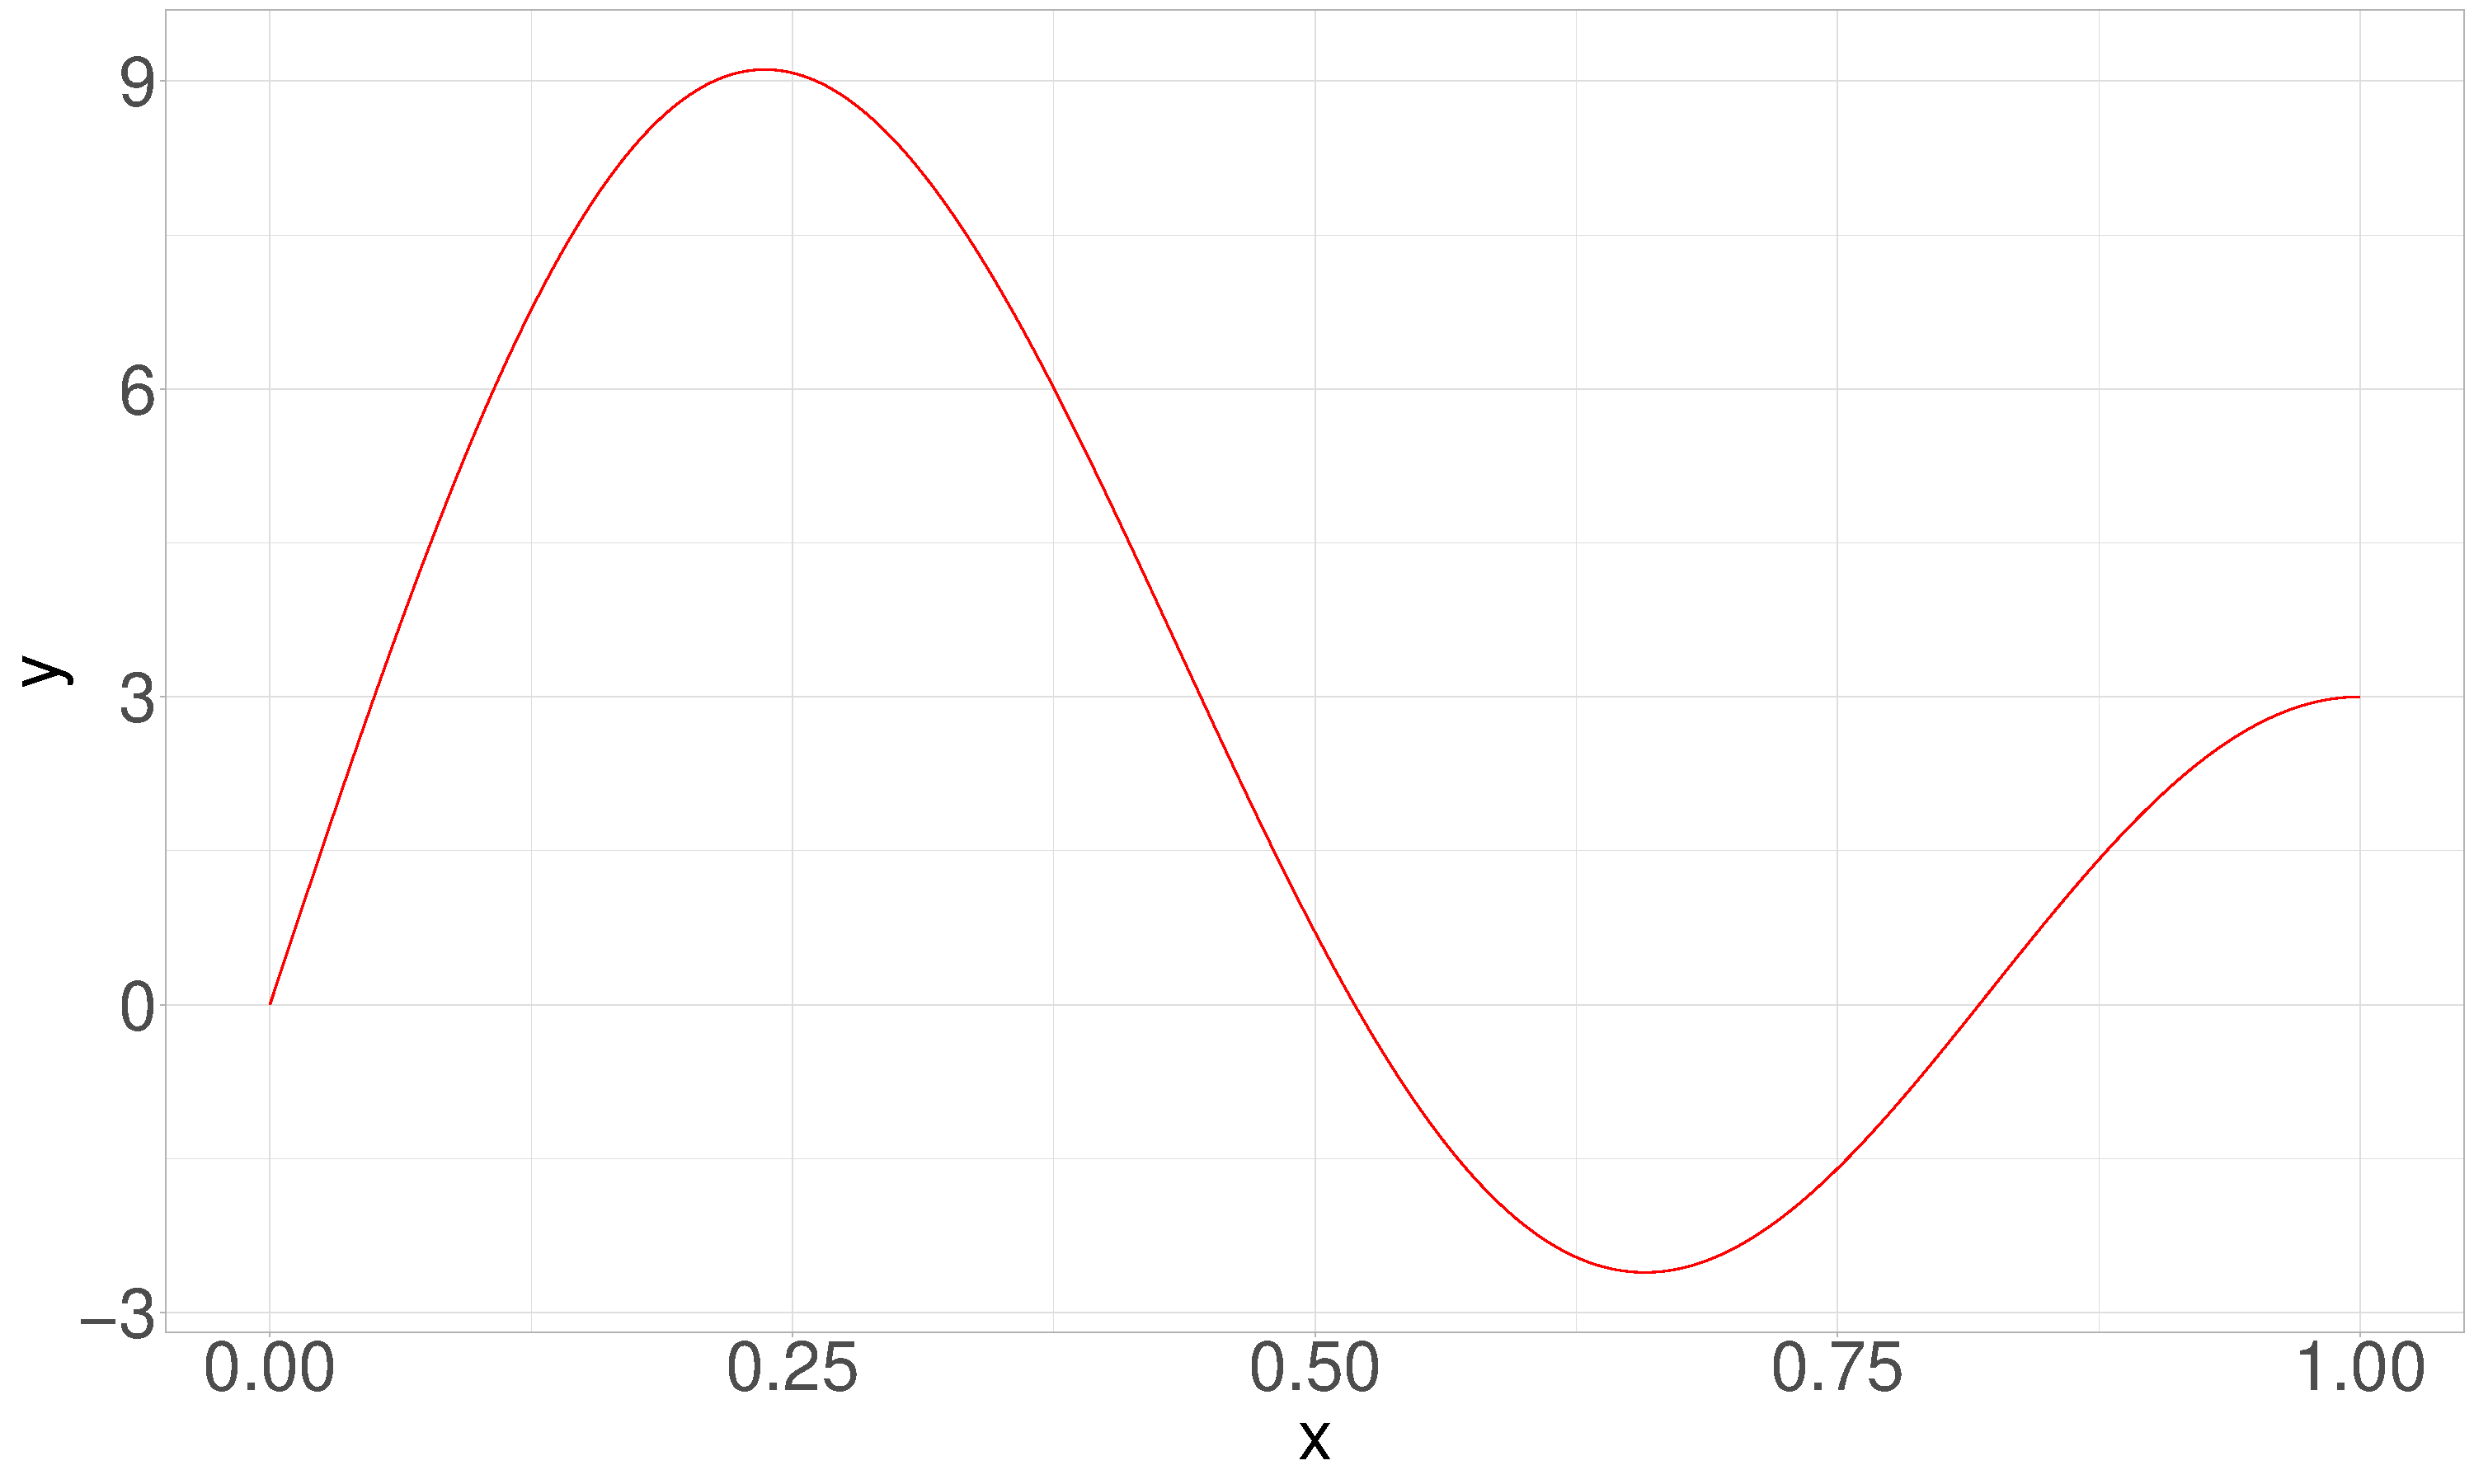
\includegraphics[width=\textwidth]{../Graphics/f1_plot.pdf}
  				\caption{$f_1(t)$, smooth function}
  				\label{fig:test1}
			\end{minipage}%
			\begin{minipage}{.5\textwidth}
	  			\centering
  				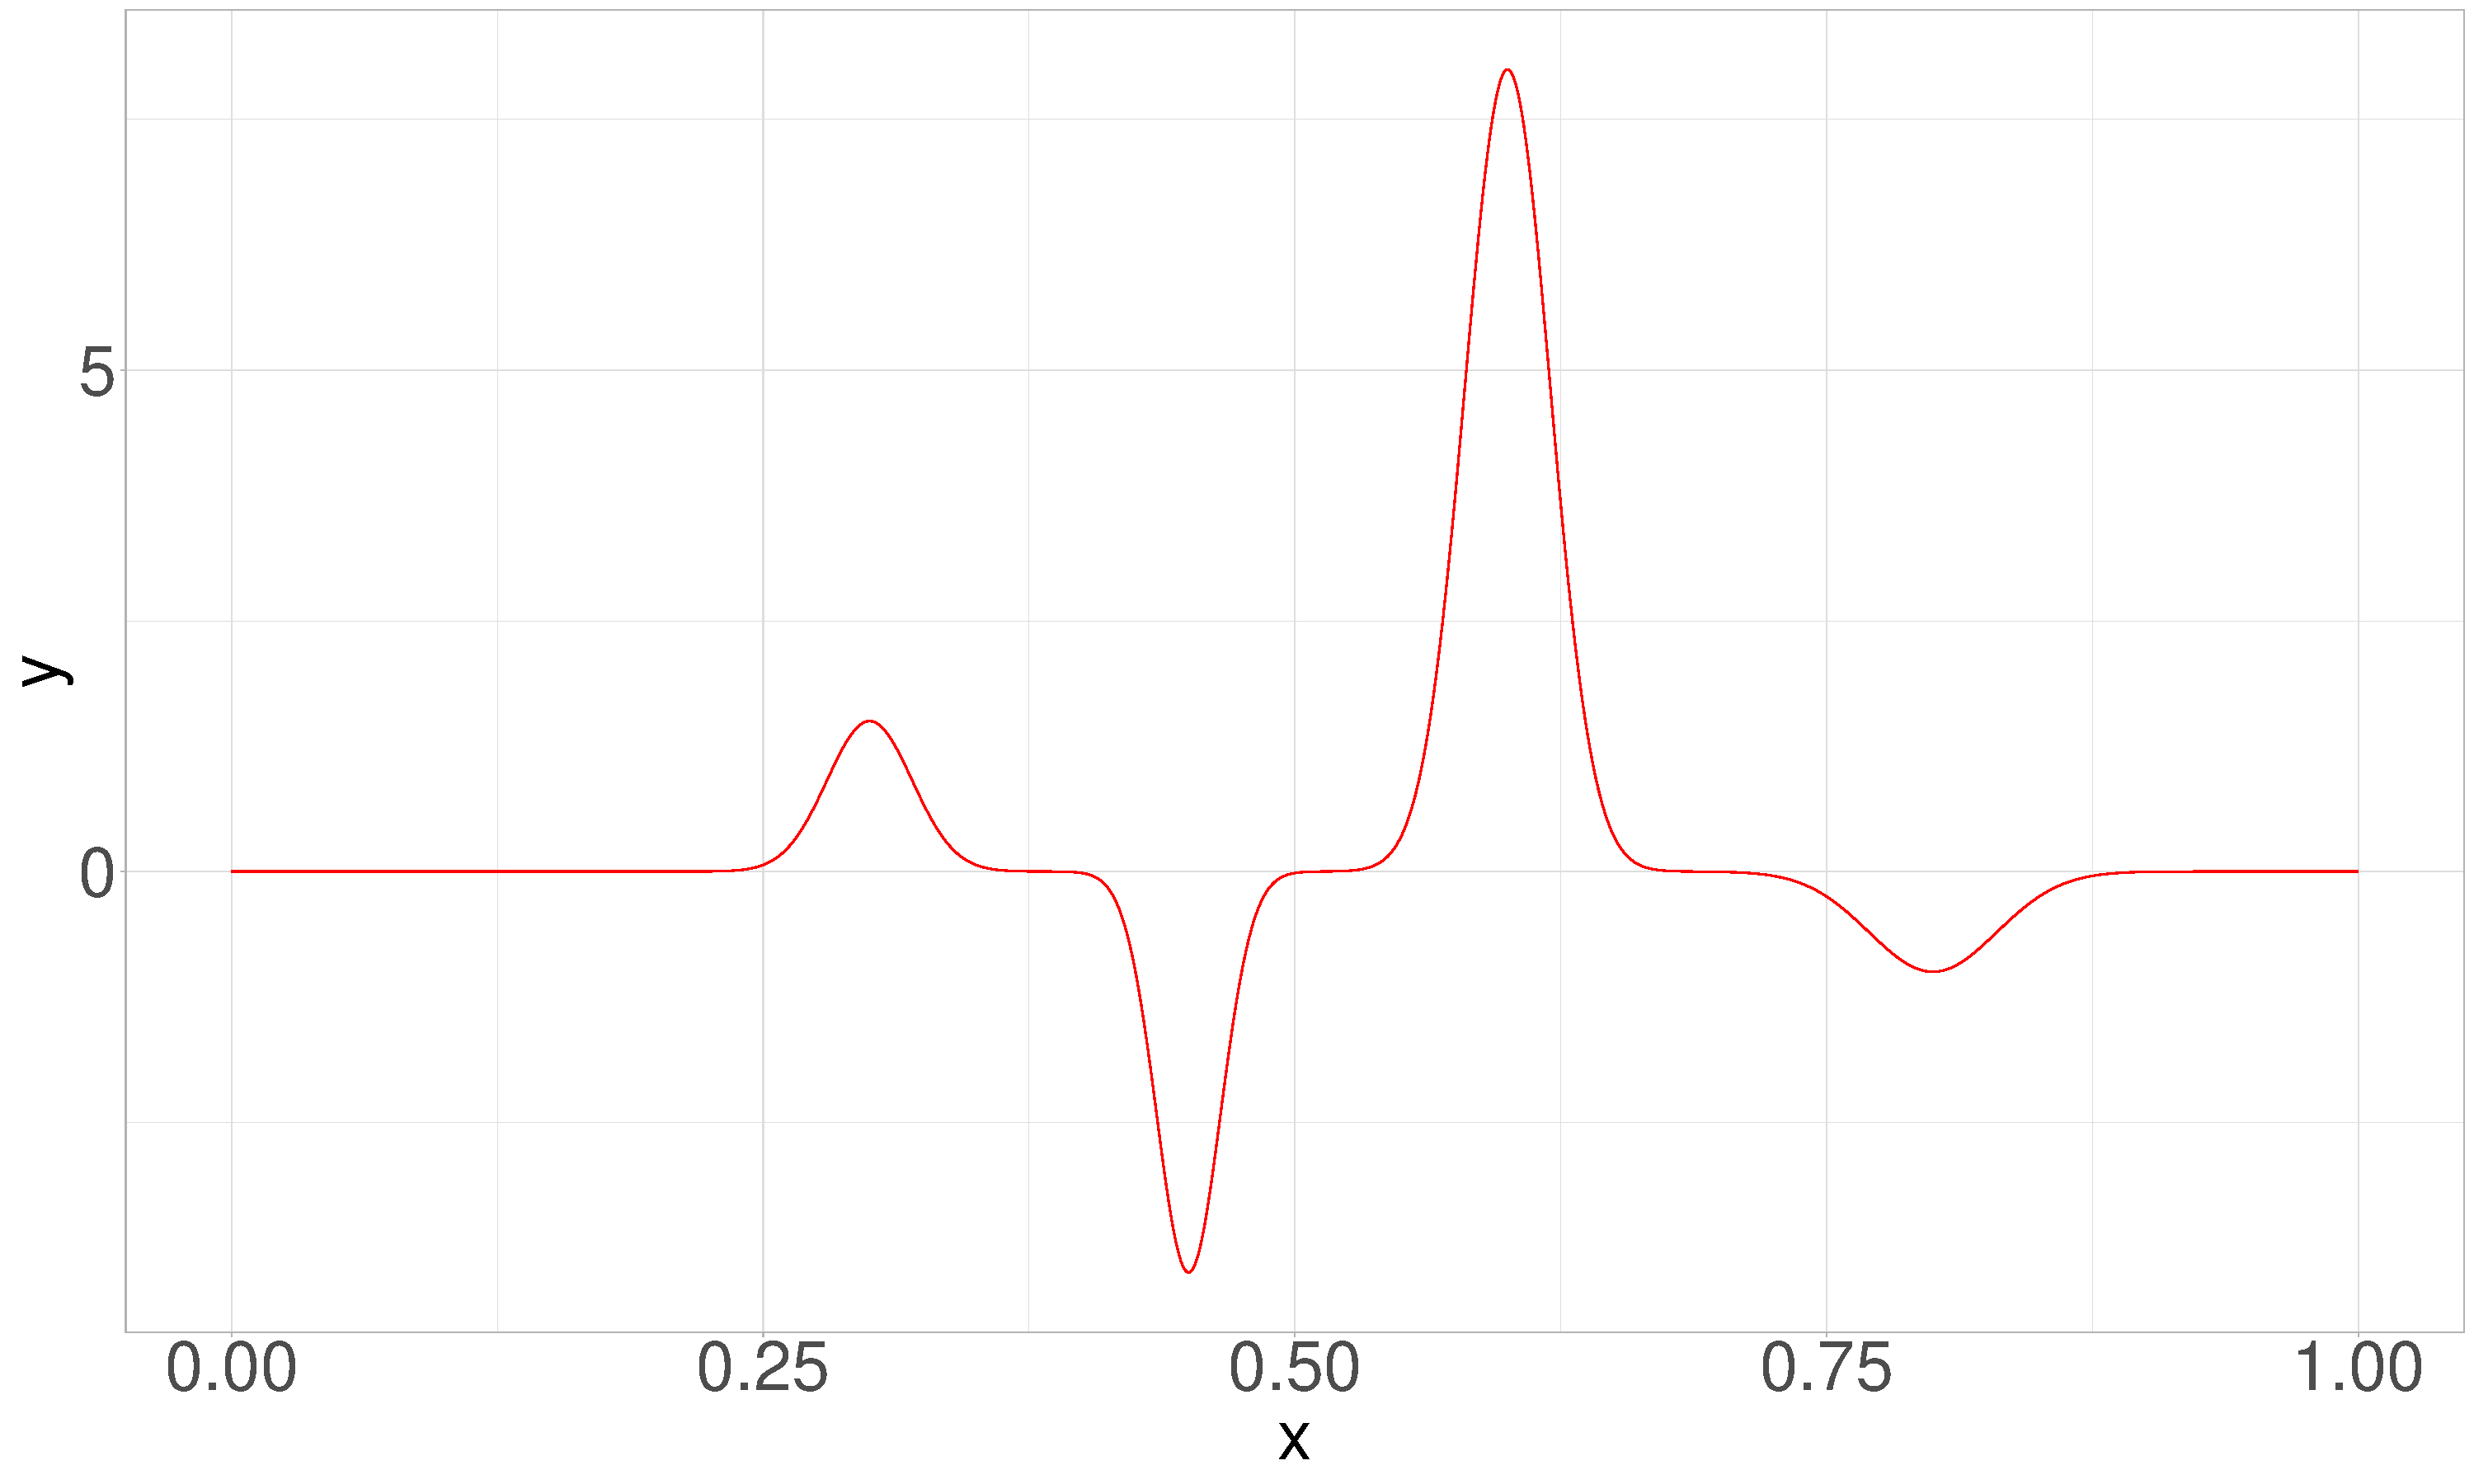
\includegraphics[width=\textwidth]{../Graphics/f2_plot.pdf}
  				\caption{$f_2(t)$, bumpy function}
  				\label{fig:test2}
			\end{minipage}
		\end{figure}
		
		 Two different error-terms $\epsilon$ were created by first generating an i.i.d. standard normal error term and then multiplying it by two error variations $\sigma_e $. The error variations represent different signal-to-noise ratios to test the methods with low and high amounts of noise. They are created such that the squared multiple correlation coefficient $R^2 = var(\langle X, f\rangle) / (var(\langle X, f\rangle) + \sigma^2_{e})$ is equal to 0.9 and 0.6. The two error terms are then used to generate two sets of responses for $f \in \{f_1(t), f_2(t)\}$	
		\begin{equation}
			\begin{split}
				Y_{1,f} & = \langle NIR, f\rangle + Z  \biggl\lbrack\frac{var(\langle NIR_{sim}, f\rangle)}{0.9} - var(\langle NIR_{sim}, f\rangle)\biggr\rbrack \\
				Y_{2,f} & = \langle NIR_{sim}, f\rangle + Z  \biggl\lbrack\frac{var(\langle NIR_{sim}, f\rangle)}{0.6} - var(\langle NIR_{sim}, f\rangle)\biggr\rbrack
			\end{split}
		\end{equation}
		
		where $Z \sim \mathcal{N}(0,1)$. In total, we created four combinations, using the two true coefficient functions and the two error terms. These four combinations are then used with a different number of monomial basis functions $ \in \{1,2, \dots, 6\}$, cubic B-spline basis-function $\{5,6,...,18\}$ and Fourier functions $\{1,3,...,25\}$ to predict the generated responses using the basis expansion approach and the FPCR approach. For the evaluation, we used the prediction MSE calculated by 10 fold cross-validation.
		To obtain valid out of sample properties for the FPCR, within each of the ten ten-fold cross-validation splits, we first calculate the first $nharm$ FPC's for $nharm \in \{2,3,4\}$ of the training set $\mathcal{T}$, which was smoothed with the respective basis function specification. The obtained Eigenfunctions $\nu^{m,\mathcal{T}}$ are then used to estimate the scores of the holdout set $\mathcal{H}$, $\hat{\xi}_{i}^{m, \mathcal{H}}$  by the equation
		\begin{equation}
			\begin{split}
				\hat{\xi}_{i}^{m, \mathcal{H},L} & =  \int_{0}^{1} {\color{red} \left(X_{i}^{\mathcal{H}}(s) - \hat{\mu}^{\mathcal{T}}(s)\right)} {\color{blue}\tilde{\nu}^{m, L, \mathcal{T}} }\mathrm{d}s) 
			    \approx \int_{0}^{1} {\color{red}\left(\sum_{j = 1}^{L} a_{i,j}^{\mathcal{H}} \phi_j(s)\right)} {\color{blue}\left(\sum_{k = 1}^{L} d_{k}^{m, \mathcal{T}} \phi_{k}(s)\right)} \mathrm{d}s \\
				 &\approx \sum_{j = 1}^{L} \left[ a_{i,j}^{\mathcal{H}}\sum_{k = 1}^{L}  d_{k}^{m, \mathcal{T}} \int_{0}^{1} \phi_j(s) \psi_{k}(s)\mathrm{d}s\right]
			\end{split}
		\end{equation}
	
		with truncation parameter $L$. In total, 5000 repetitions were conducted for each set of simulations. 
		
	\subsection{Results}	
	The discussed results and figures of $\hat{\beta}(t)$ for the simulation can be found in Appendix \ref{Tables_sim} and \ref{Estimates_sim}. 
	\subsubsection{Basis Expansion Regression}
	The following results origin from the \hyperref[basis_exp_transf]{Estimation using Basis-Representation}, in which we transform the smooth curves to perform FLR. Examining the results, it appears that the cross-validated MSPE inherets a convex nature in the increasing basis functions.
	
	\paragraph{Monomial Basis}
	Due to the in the number of basis functions increasing collinearity of these basis functions, simulations were conducted up until the sixth monomial, which already shows signs of numerical instability. For reasons outlined in \ref{Monomial_basis}, they seem suited for $f_1$ where it shows a better performance than B-splines for this coefficient function. A hypothesis for this could be that $f_1$ is an entire function, which can be well approximated with a power series. In case of $f_2$, this basis shows the weakest performance out of all basis, for which the plots in \hyperref[basis_expansion_2_1]{figure 9} and \hyperref[basis_expansion_2_2]{10} provide evidence. It seems like $\hat{\beta}(t)$ is not changing in the amount of noise and shows exaggerated behaviour at the boundaries. This weakness is especially pronounced in the MSPE for $f_2,Y_1$. For $f_1$, the simulation selects 5(3) and for $f_2$ 5(5) monomial basis functions for the high(low) signal-to-noise ratio. 
	\vspace{-0.2cm}
	
	\paragraph{B-spline Basis}
	Simulations with B-spline basis functions were possible from 4 to 18, since from 18 onwards the simulations were running into collinearity problems.
	Function $f_1$ requires 5(4) B-spline basis functions, for the high(low) signal-to-noise ratio to obtain the best fit for the B-spline basis. It still performs the worst for $f_1$. An explanation might be its exaggerated behavior at the boundaries and the exaggeration of the peculiarities of $f_1$ (\hyperref[basis_expansion_1_1]{ADD} and \hyperref[basis_expansion_1_2]{ADD}), which is especially pronounced for the lower signal-to-noise ratios. For $f_2$, 11(6) B-spline basis functions are chosen for the high(low) signal-to-noise ratio. For $f_2$, the B-spline basis outperforms the monomial basis but comes second to the Fourier basis. While the basis seems to recognize the peculiarities in $f_2,Y_1$, it seems to struggle with it for the noisy responses in $f_2,Y_2$ ((\hyperref[basis_expansion_2_1]{ADD} and \hyperref[basis_expansion_2_2]{ADD})).
	\vspace{-0.2cm}
	
	\paragraph{Fourier Basis}
	For $f_1$, the simulation chooses a smaller number of Fourier basis functions, 5(3) and a higher number for $f_2$, 9(7) for the setup with the high(low) signal-to-noise ratio. With the low signal-to-noise ratio in the responses, the simulation chooses a smaller number of basis functions, which could be to prevent fitting this scalar noise using $\hat{\beta}(t)$. The Fourier basis functions perform the best for each setup for the basis expansion regression. Several reasons could contribute to this: First, especially $f_1$ shows similar curvature order across the domain while the curvature of $f_2$ does at least not display any erratic jumps. Second, both functions feature periodic behavior. Third, $f_2$ does have the same value at the start- and the end of the interval lending itself to a periodic representation.	\\
	
	\subsubsection{Functional Principal Component Regression}
		The model used for the FPCR is described in \hyperref[fpc_exp_transf]{Estimation using Functional Principal Components}. In addition to the selection of the truncation parameter $L$, the choice of the number of FPC's adds to the complexity of the model since the approximated Eigenvalues and -functions from the decomposition are influenced by the choice of $L$ that was used to expand the function. But since the FPCR is ultimately estimated with a linear model with the corresponding scores as regressors, the relevant degrees of freedom in the estimation of the ultimate model are not affected by $L$, but only by the number of FPC's $n_{FPC} \in \{2, 3, 4 \}$. As will be described, it seems that neither a convex behavior of the MSPE, nor any clear relationship can be observed between the number of basis function and the number of FPC's. This might be because the dependency (FPCA is performed on the smoothed curves) is to complex to draw conclusions from this simulation study, therefore we will limit ourself to a brief description. In this simulation, the cross-validated choice of basis functions indicates that the FPCR might not take the differing signal-to-noise ratios of the responses into account since the FPC's, which affect the relevant degrees of freedom, are calculated solely from the smoothed curves, not considering the noise in the responses at all.
	
	\paragraph{Monomial Basis}
	For $f_1$, the cross-validated MSPE is decreasing in the number of FPC's and chosen basis functions for both the high and the low signal-to-noise ratio (4,5,6 basis functions for $n_{FPC} \in \{2, 3, 4 \}$). In  $f_2$ we also observe a decreasing MSPE in the number of FPC's, but no clear relationship for the chosen basis functions. The monomial basis shows the weakest performance for all three basis functions in each setting for all $n_{FPC}$.
	\vspace{-0.2cm}
	
	\paragraph{B-spline Basis}
	For $f_1,Y_1$, the MSPE suggests that models with a higher number of FPC's perform better. While the number of basis functions stays at five for $n_{FPC} = 2,3$, it increases to 6 basis functions for $n_{FPC} = 4$. In $f_1,Y_2$, the cross-validated MSPE is only slightly affected by $n_{FPC}$, but lowest for $n_{FPC} = 3$, indicating the possibility of overfitting using $n_{FPC} = 4$. Similar to the two setups with $f_1$, the cross-validated number of basis functions for $f_2$ is increasing in the number of FPC's (4, 6, 23 for $n_{FPC} \in \{2, 3, 4 \}$)
	\vspace{-0.2cm}
	
	\paragraph{Fourier Basis}
	In $f_1,Y_1$, the MSPE is decreasing in $n_{FPC}$ while the results in $f_1,Y_2$ might indicate overfitting when using $n_{FPC} = 4$. $f_2,Y_1$ displays the greatest relative decline of MPSE in the increasing number of FPC's, but in absolute values, therefore acknowledging the higher noise responses for $f_2,Y2$, the decline of MSPE is similar to the decline observed for $f_2,Y_2$. Both configurations of $f_2$ are using 5, 15 and 7 basis functions for $n_{FPC} \in \{2, 3, 4 \}$.
	\vspace{-0.2cm}	
	
	\subsubsection{Interpretation and Relevance for Application}
	A possible explanation applicable to the setups performing Basis Expansion Regression might be the effect of the Bias-Variance tradeoff and the following hypothesis: For $f_1$ only little bias seems to be introduced when choosing a small number of basis functions. For $f_2$, a higher number of basis functions seems appropriate, resulting from the inherent peculiarities of $f_2$ that are more pronounced with higher $L$. This results in higher numbers of basis functions since the bias is decreasing faster than the variance is increasing in the number of basis functions compared to $f_1$. The uncovered and described convex behaviour of the MSPE also might partly attributed by the bias-variance tradeoff. 
	
	This convex behavior was not observed for the FPCR where no clear relationship between the basis functions and the number of FPC could be uncovered. An hypothesis for this is that the dependency between the truncation parameter $L$ and the FPC's, which are calculated from $L$-truncated smoothed curves, is too complex to capture in our setting. To examine this further, additional simulations were conducted for B-spline basis functions with a large truncation parameter $L \in \{50, 70\}$ for $n_{FPC} \in \{2, \dots, 7 \}$ (LINK TO APPENDIX). As in the simulation study we can find potential signs of overfitting for all setups and both choices of $L$. The additional simulations revealed evidence that there might exist a relationship from $n_{FPC} = 3$ onwards: For $n_{FPC} \in \{3, \dots, 7 \}$, the 10-fold cross-validated MSPE is always lower for 50 than for 70 basis functions which might be a first sign of a too high $L$ and subsequent undersmoothing. Following this, it seems that once a sufficient number of basis functions is used to expand the curves, the FPCR performs better using a more conservative number of basis functions (here $L = 50$). The settings $f_1,Y_2$ and $f_2,Y_2$ perform worse for these high number of basis functions, while $f_1,Y_1$ and $f_2,Y_1$ show a stronger performance than in the main simulation study, although the signal-to-noise ratios of the responses are not affecting the construction of the FPC's which might indicate beneficial attributes of the lower truncation parameters used in the main simulation.
	
	%Keeping \cite{Jolliffe_1982} in mind, we ....(refer to problematic of missing insights in pysics / chemistry?)
	


	\section{Application}\label{Application}
		Our application uses the methods and insights from the previous sections to predict the octane ratings of the  gasoline data set.
		Although the simulation study granted valuable insights into the different methods in our four different settings, it is not enough to determine the optimal method and choice of basis for the application, since there is too much uncertainty involved. To point out some sources of uncertainty: First, differing from the simulation setup, we do not know the true coefficient function. Visual inspection of the the estimated coefficient functions shown in Appendix \ref{Estimates_Appl} fuels the hypothesis the real coefficient function might be more similar to $f_2$ than to $f_1$ but the insights from two functions are not sufficient to draw any conclusion. Second, we have no information about the signal-to-noise ratio of the measured octane numbers. Third, to generate similar curves, we made assumptions about the distribution of $\mathring{\xi}$ that are not applicable in this application where we do not know their distribution.
		 
		Therefore, we will rerun all specification for the gasoline data set and use the results of the simulation study to improve our understanding of the results. The application is designed analogously to the simulation study: The 60 spectra of the gasoline data set will be used to estimate a coefficient function, predict the reported octane numbers, and evaluate the results via prediction MSE using 12 fold cross-validation with 5 elements per fold. In total, we conducted 1000 repetitions for each setting.
		

		
	\subsection{Interpretation of Results}
		\subsubsection{Basis Expansion Regression}
		The cross-validated MSPE selects 5 basis functions for the monomial basis. For B-Splines, the cross-validation selects 10 basis functions and 9 basis functions for the Fourier basis. Comparing the estimates in Appendix \ref{Estimates_Appl}, away from the boundaries, the B-spline and Fourier bases show similar behavior, opposing to the monomial estimate which might be attributable to the lower number of basis functions. Especially at the lower boundary, the monomial basis shows an exaggerated behavior. However, we must exercise caution since from $L=6$ onwards, we were not able to calculate stable results for the monomial basis. The MSPE for B-splines (0.04574) and Fourier (0.04808) are similar while the monomial basis (0.24181) shows distinctly worse properties. In contrast to the simulation study, the B-splines basis manages to outperform the Fourier basis. Driving factors for this better performance could be that, first, we do not assume a periodic true coefficient function with the same start- and end value and second, that the Fourier basis enforces identical start and end value on $NIR$. It is worthy to note that the reported MSPE for the B-spline and Fourier basis are close to the errors reported in the simulation study for the setup $f_2,Y_1$, which might be caused by the hypothesized similarities between the true coefficient function and $f_2$, but also by a similar high signal-to-noise ratio of the octane numbers. 
	
		\subsubsection{Functional Principal Component Regression}
		The best performance for all numbers of FPC's was achieved with the Fourier Basis, as for the FPCR in the simulation study. In contrast to the simulation study, no evidence of overfitting was found for the best basis choices in any of the three bases. The MSPE for the optimal specification appears to be strictly decreasing in the number of FPC's. As for the simulation study, the interpretation of the results with respect to the chosen basis is difficult: Referring to the plotted estimates $\hat{\beta}(t)$ in \hyperref[FPCR2_estimate_appl]{ADD}, \hyperref[FPCR3_estimate_appl]{ADD} and \hyperref[FPCR4_estimate_appl]{ADD}, it appears to be the case that the higher $n_{FPC}$ is, the more similar behavior of the estimate $\hat{\beta}(t)$ can be observed. Differing from the simulation study, the number of basis functions is steadily increasing for the monomial basis. The behavior for the B-spline basis is similar to the one reported in the simulation study (basis functions increasing in $n_{FPC}$). 
	

	%\nocite{carey_life_2002}

	\section{Outlook}\label{Outlook}
	
	\subsection{Limitations}
	
	\paragraph{Insights from Simulation cannot be Extended to More General Functions}
	\vspace{-0.2cm}
	
	\paragraph{Collinearity Problems in Basis Expansion Regression}
	As already described in the section on the simulation study, the basis expansion regression was in part limited by the numerical instability of the estimation procedure. This is mainly due to an increase in collinearity of the derived regressor matrix shown in Definition \ref{regressor_mat_1}. This problem is inherent to basis systems whose functions are not pairwise orthogonal, such as the monomial or B-splines bases, but gets more pronounced the more functions we add to the basis system and the higher the correlation between those functions. \\
	The numeric instability of the inversion of this matrix makes the estimates unreliable and therefore can make this approach infeasible for non-orthogonal bases in settings where the characteristics of the data set demand a higher number of basis functions than is feasible due to the properties of the estimation procedure.
	\vspace{-0.2cm}
	
	\paragraph{Low Number of Basis Functions in FPCR Regression}
	Another limitation of the exploration into functional principal component regression is the low number of principal component specifications used in this paper. As the simulation and application showed, the number of basis functions does not seem to be the deciding factor for the performance of this method as long as an appropriately high number of basis functions is provided. 
	A more significant factor seems to be the number of principal components available for the linear regression which in itself could be subject to choice according to cross validation.
	\vspace{-0.2cm}
	
	\subsection{Possible Extensions}
	
	\paragraph{Orthogonal Polynomials to Solve Collinearity Problems of Monomial Basis}
	To address the collinearity problems described earlier, one possible idea would be to use a system of pair-wise orthogonal polynomials as a basis instead of the monomial basis. One example is the system of Legendre polynomials which are orthogonal by construction and have the same closed span as the monomials. Due to their orthogonality, the problem of collinearity in the regressor matrix are greatly reduced which could allow for larger numbers of basis functions in the basis expansion regression approach. The first eight Legendre polynomials are shown in Appendix section \ref{Basis_Plots}.
	\vspace{-0.2cm}
	
	\paragraph{Comparison to Penalty Based Smoothing Procedures}
	In contrast to the more typical approach of using a large but often arbitrary number of basis functions and smoothing using a penalty term involving for example the second derivative of the curve, this paper focuses on smoothing by using a smaller number of basis functions. As a next step to the analysis of this paper, it would be interesting to compare both methods to see in which settings different approaches to smoothing perform better and if a possible combination of both approaches could be advantageous.
	\vspace{-0.2cm}
	
	\paragraph{Larger Range for the Number of Specifications for FPCR}
	\vspace{-0.2cm}
	
	\paragraph{Input from Physics Analysis}
	It would be interesting to combine the purely mathematical findings of this paper with theoretical expertise from the field of physics as this could inform the choice of models and be conducive to a more meaningful interpretation of estimates. For example, specific parts of the NIR spectrum can possibly be liked to specific molecules associated with a high predictive power for the octane value. This could guide, for example, the construction of a B-spline basis that focuses on the relevant parts of the spectrum by using a vector of knots founded by field expertise. Alternatively, it could be used to link specific principal components to compounds which would be interesting for the interpretation of estimates.
	\vspace{-0.2cm}
	
	\nocite{James.2009} %(shape-restrictions)
	
	\newpage
	\section{Appendix}
	
	\subsection{Near-infrared (NIR) Spectroscopy}\label{NIR}
	NIR- spectroscopy is a spectroscopic method that uses the near-infrared region of the electromagnetic spectrum (From 780 nm to 2500 nm). It, therefore, measures the absorption and interaction of this spectrum of radiation with the sample. NIR-spectroscopy is not only faster and cheaper than the standard test procedure – another significant advantage is that it does not need a reagent and thus does not destroy the sample. It is used for analysis in different sectors and fields, like the agrochemical industry and healthcare. Its non-invasive nature makes it also an asset for medical applications like the monitoring of diabetes in which NIR-spectroscopy can detect the worsening of the blood glucose metabolic dysfunction (cf . \cite{FR_li_et_al_2020}). \\
	In the context of this paper, the gasoline data set which is used for the simulation and the application is constructed using NIR spectroscopy. According to \cite{Bohacs_Ovadi_Salgo1998} NIR-spectroscopy is a feasible method for the analysis of gasoline since most of the absorption that is observed within the described interval of wavelengths is due to overtones and interactions of the radiation with chemical combinations (carbon–hydrogen, carbon–carbon, carbon–oxygen, carbonyl associated groups, aromatic stretching, and deformation vibration of the hydrocarbon molecules). While this paper focuses on the prediction of the octane number of gasoline, other research focuses  on different properties of gasoline such as the olefin, naphtaenic and aromatic content (Parisi et al. 1990, as cited in \cite{Bohacs_Ovadi_Salgo1998}) or the distillation characteristics (Pauls 1985, as cited in \cite{Bohacs_Ovadi_Salgo1998})
	\vspace{0.5cm}

	\begin{figure}[H]
		\begin{center}
			\begin{overpic}[width = \textwidth]{../Graphics/NIR_data.pdf}
				\put(7, 30){
					\frame{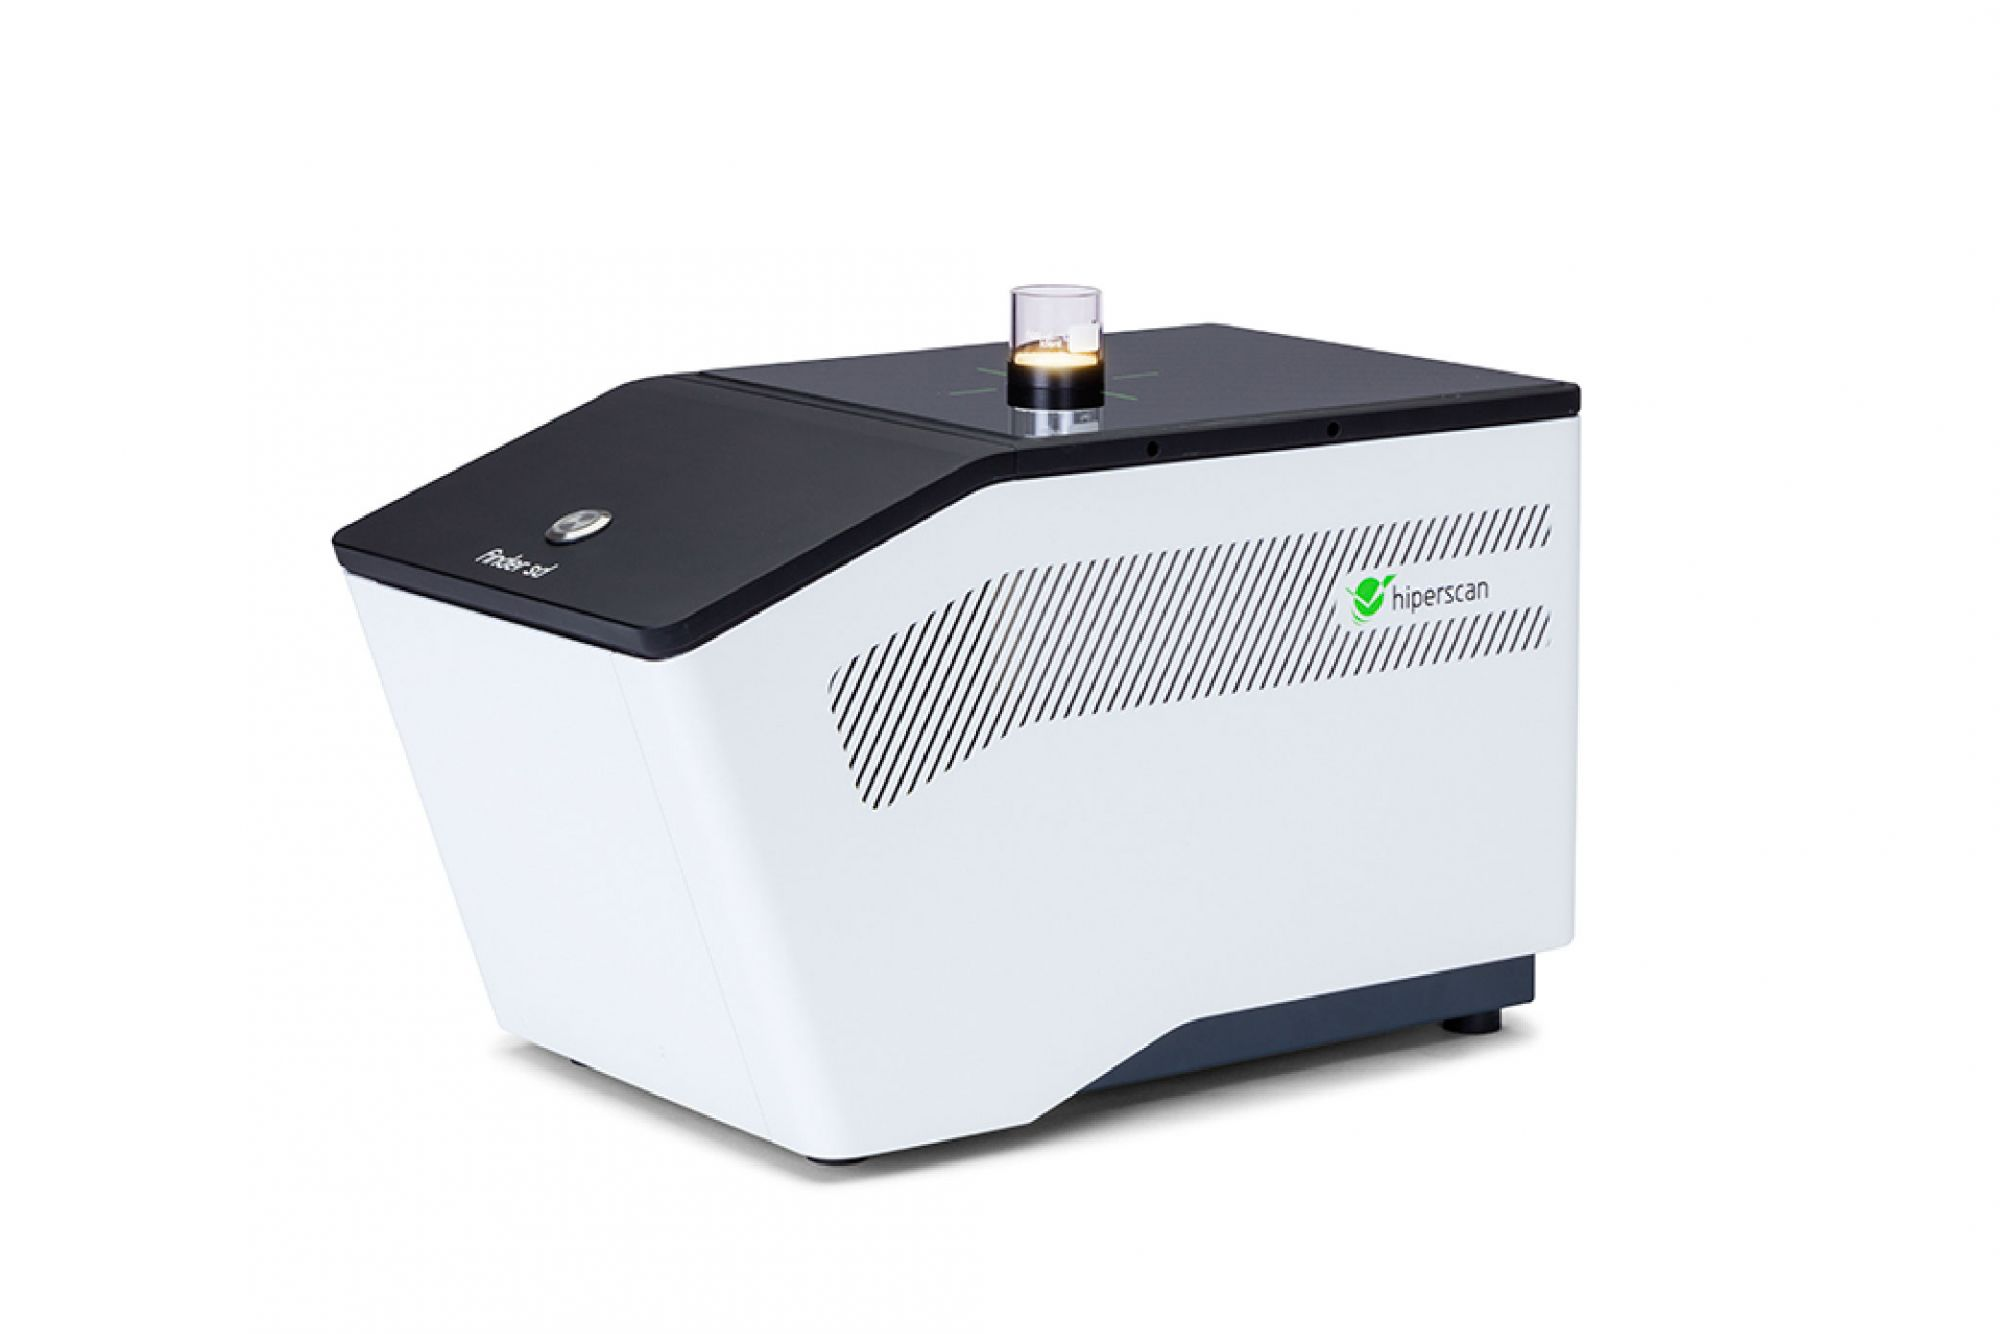
\includegraphics[width = 0.4\textwidth]{../Graphics/FinderSD.jpg}}
				}
			\end{overpic}
			\caption{NIR absorption spectra from the Gasoline Data Set and Finder SD (a Near-Infrared-Spectroscope built by HiperScan GmbH)	\\
			(Source: https://www.hiperscan.com/files/apoident/uploads/Bilder/Neue\_Website/Produkte/FinderSD.jpg)}
		\end{center}
	\end{figure}

	\newpage
	
	\subsection{Basis Plots}\label{Basis_Plots}
	
	\begin{figure}[H]\label{Fourier_basis}
		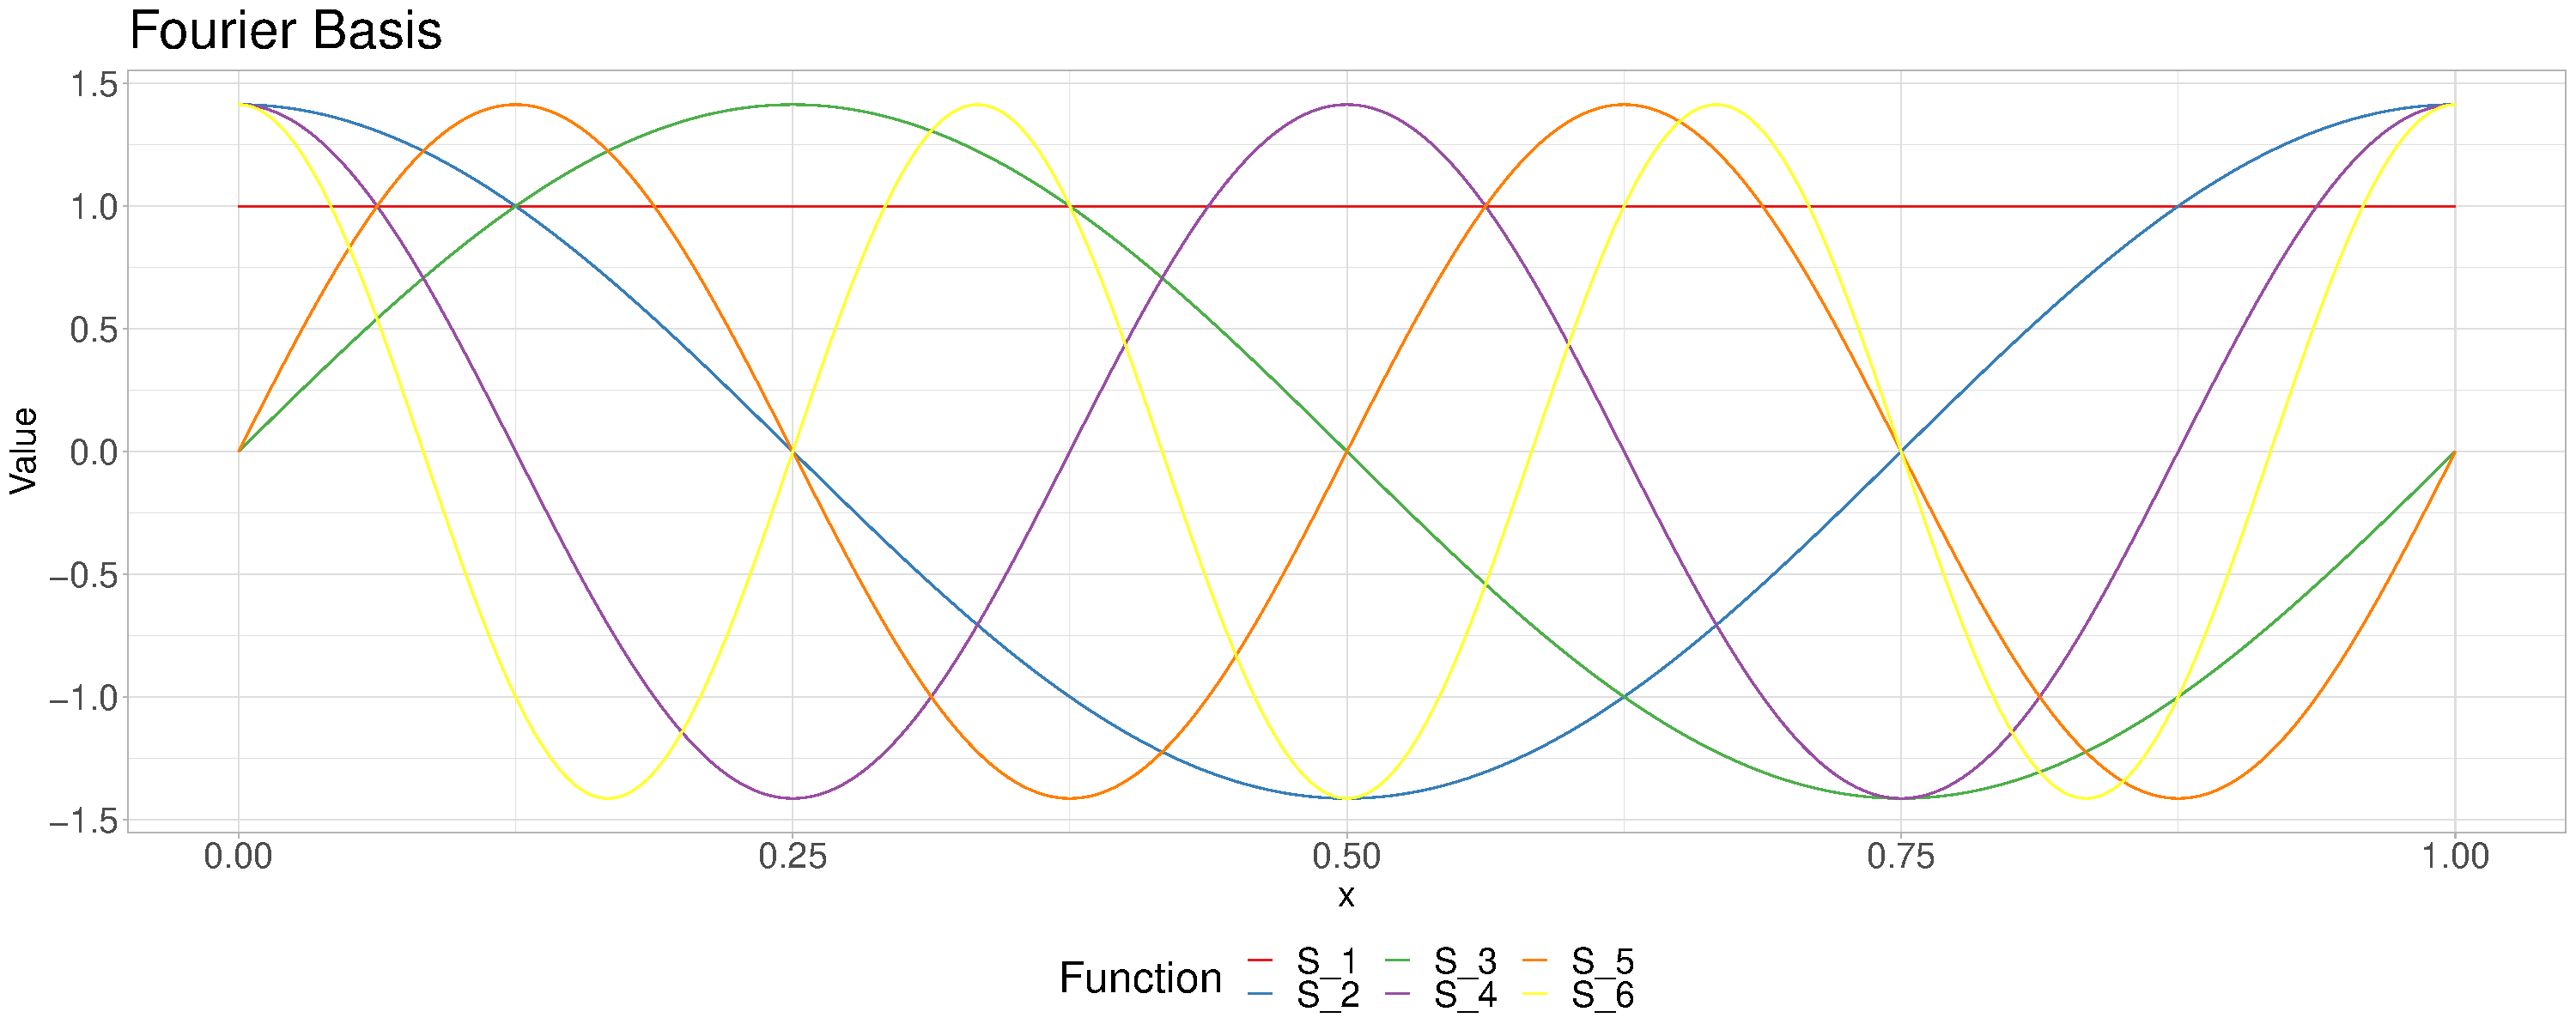
\includegraphics[width = \textwidth]{../Graphics/Fourier_Basis.pdf}
		\caption{Fourier basis functions for $i = 1,\dots,7$}
	\end{figure}
	
	\begin{figure}[H]\label{B-spline_basis}
		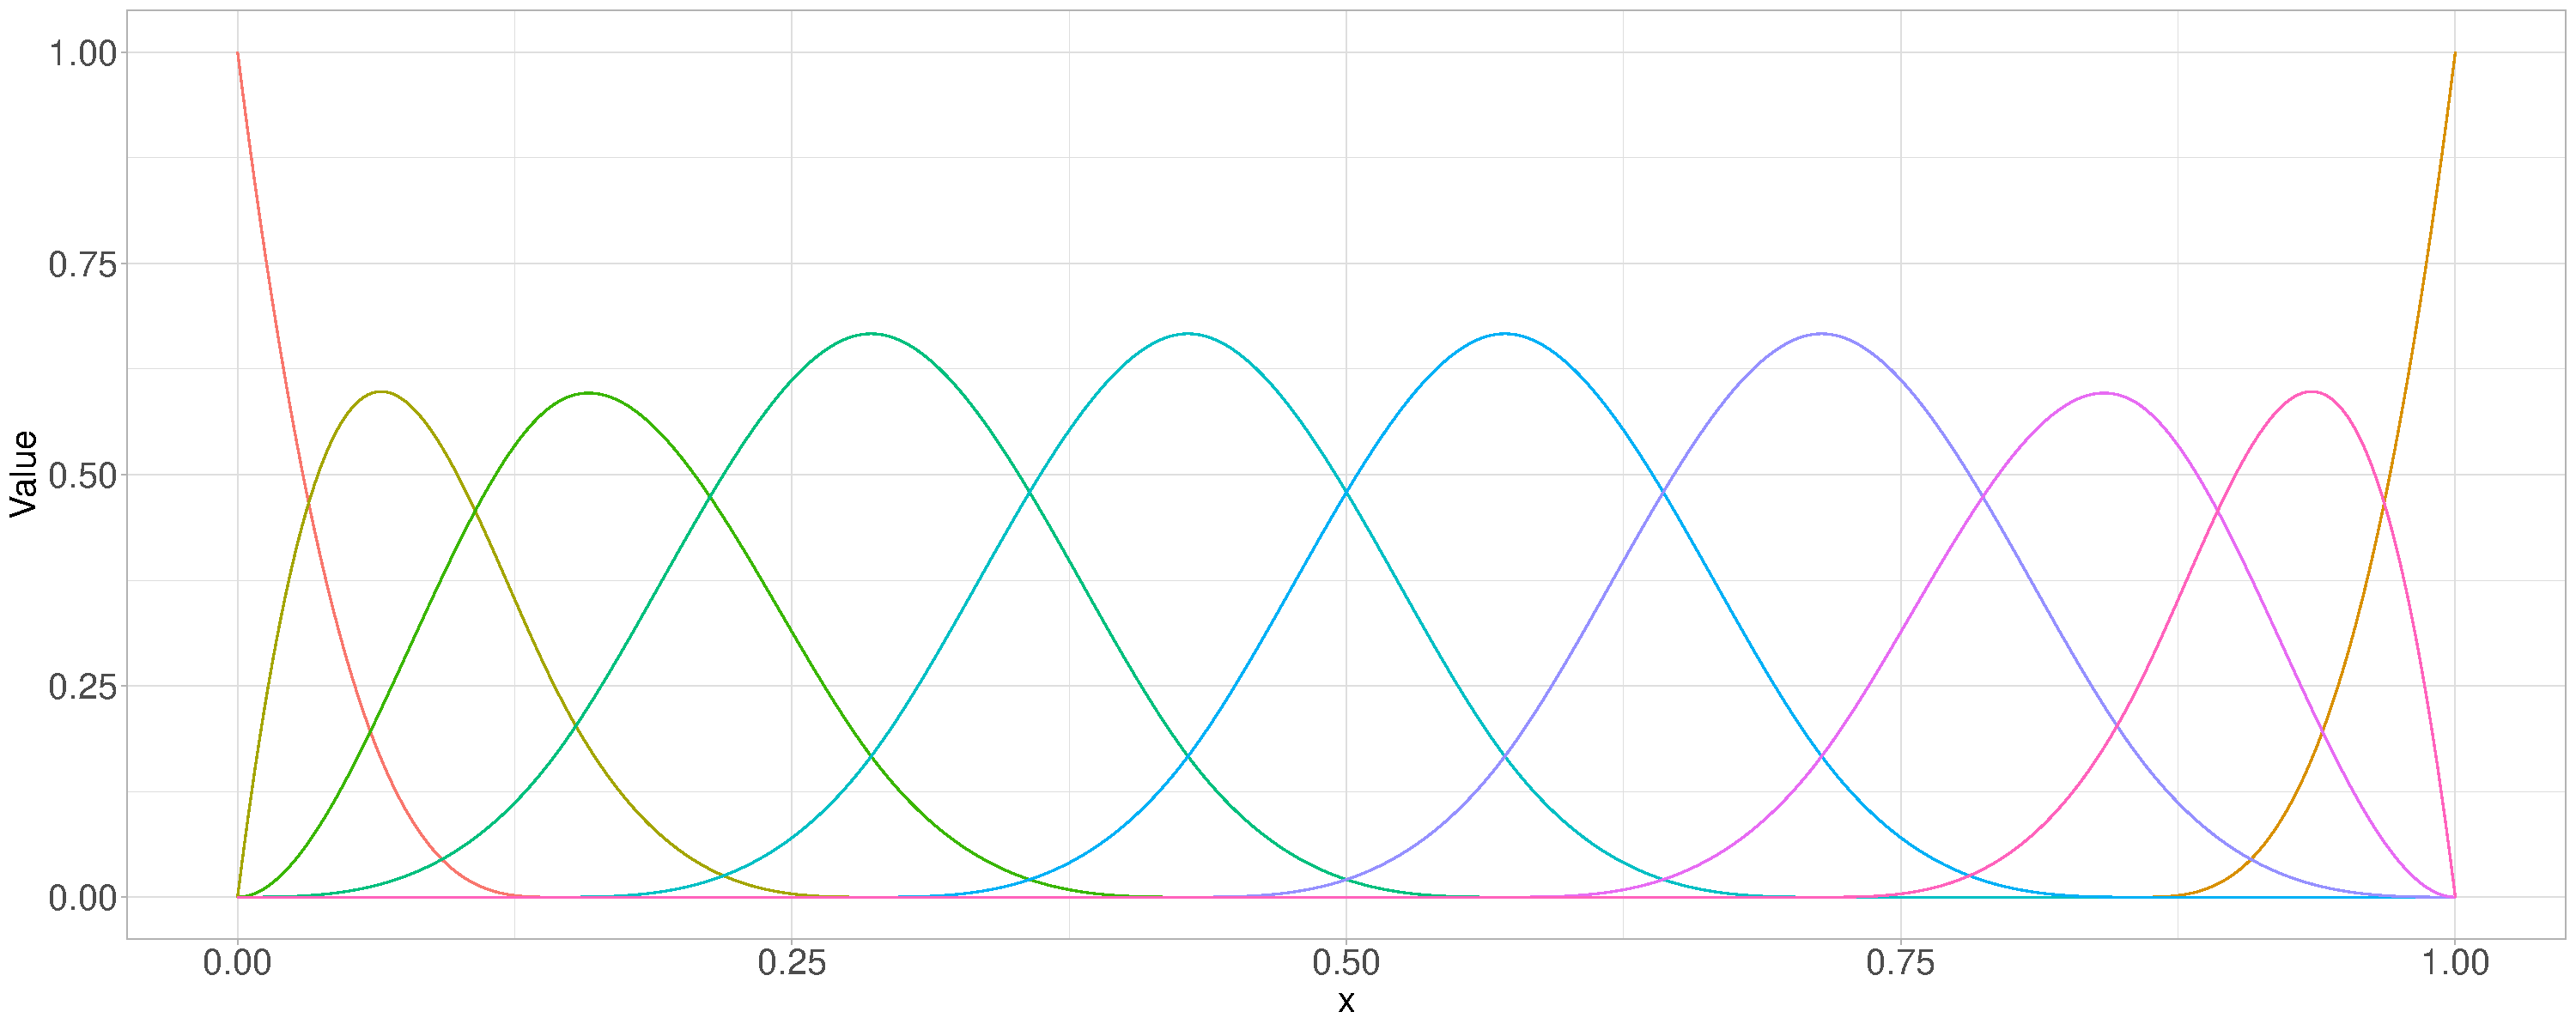
\includegraphics[width = \textwidth]{../Graphics/Bspline_Basis.pdf}
		\caption{B-spline basis functions of order 4 for 8 equidistant knots on $[0,1]$}
	\end{figure}

	\begin{figure}[H]\label{monomial_basis}
		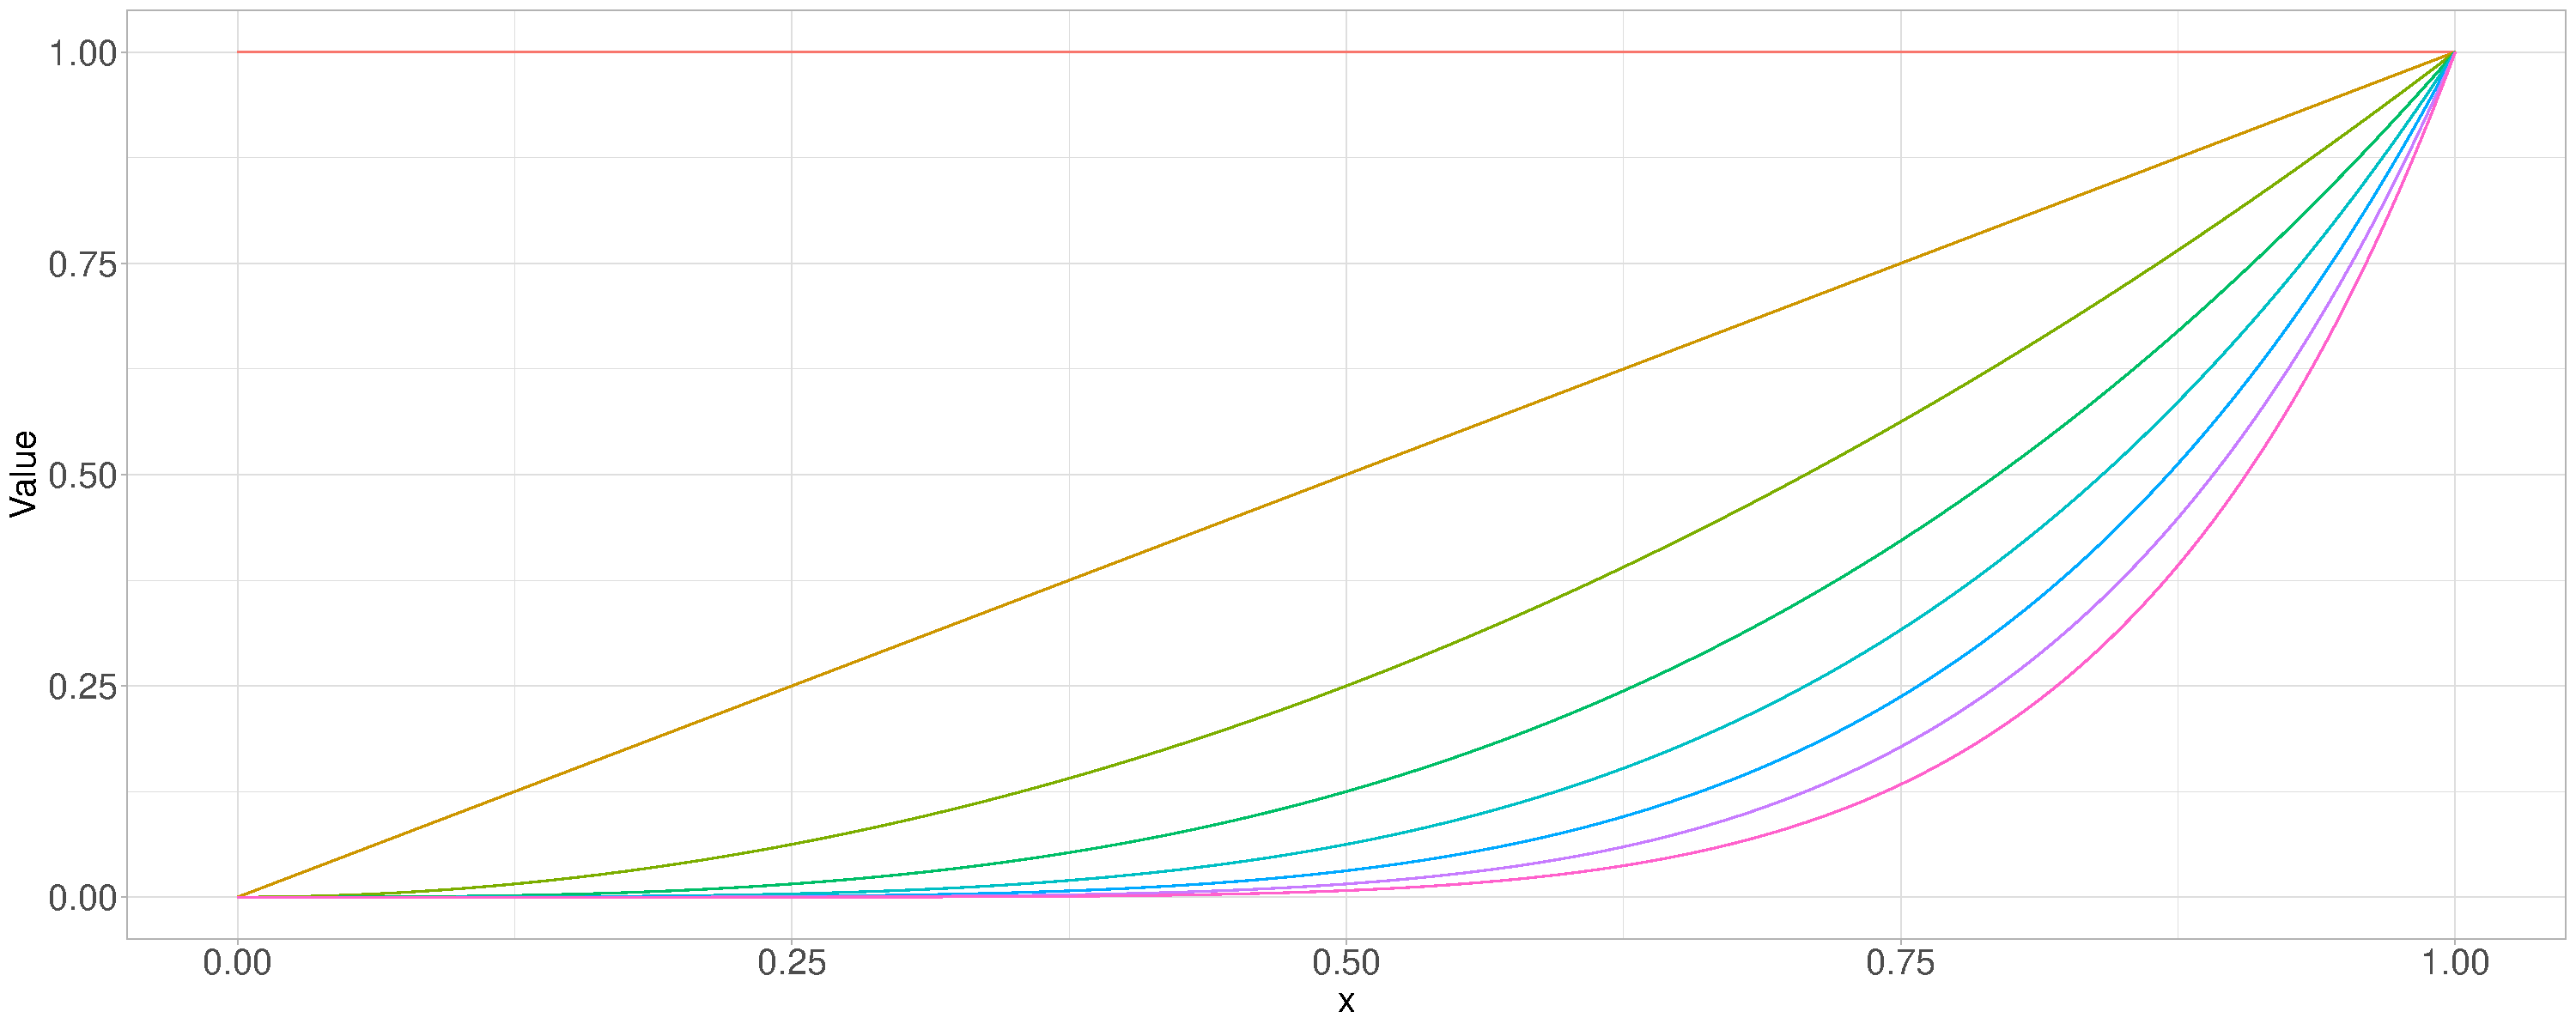
\includegraphics[width = \textwidth]{../Graphics/Monomial_Basis.pdf}
		\caption{Monomial basis functions of degree 0 to 7}
	\end{figure}

	\begin{figure}[H]\label{Legendre_basis}
		\includegraphics[width = \textwidth]{../Graphics/Legendre_Plot.pdf}
		\caption{Legendre Polynomials of degree 0 to 7}
	\end{figure}

	% extrernal file for all tables Tables


\subsection{Simulation Study Results}\label{Tables_sim}
%%%%%%%%%%%%%%%%%%%%%%%%%%%%%%%%%%%%%%%%%%%
%\begin{table}[H]
%			\centering
%			\caption{Best Model Tabel - tmp}
%				\begin{tabular}{lllllll}
%					\cline{1-5}
%					 \boldmath{$f_1, Y_1$}                 & \boldmath{$f_1, Y_2$}                  & \boldmath{$f_2, Y_1$}                    & \boldmath{$f_2, Y_2$}               & \textbf{model} &  \\ \cline{1-5}
%5     & 3     & 5     & 5     & monomial basis  \\
%5     & 4     & 11    & 6     & bspline basis   \\
%5     & 3     & 9     & 7     & fourier basis   \\
%4     & 4     & 10    & 10    & monomial fpcr 2 \\
%5     & 5     & 6     & 6     & monomial fpcr 3 \\
%6     & 6     & 8     & 8     & monomial fpcr 4 \\
%5     & 5     & 4     & 4     & bspline fpcr 2  \\
%5     & 5     & 6     & 6     & bspline fpcr 3  \\
%6     & 6     & 23    & 23    & bspline fpcr 4  \\
%3     & 3     & 5     & 5     & fourier fcpr 2  \\
%3     & 3     & 15    & 15    & fourier fpcr 3  \\
%5     & 5     & 7     & 7     & fourier fpcr 4 
%\end{tabular}
%\end{table}

%\vspace{0.5cm}	
	
	%%%%%%%%%%%%%%%%%%%%%%%%%%%%%%%%%%%%%%%
	
	

	\begin{table}[H]
			\centering
			\caption{Monomial Basis Expansion Regression}
				\begin{tabular}{lllllll}
					\cline{1-5}
					 \boldmath{$f_1, Y_1$}                 & \boldmath{$f_1, Y_2$}                  & \boldmath{$f_2, Y_1$}                    & \boldmath{$f_2, Y_2$}               & \textbf{n\_basis} &  \\ \cline{1-5}
7.17723                       & 131.92717                        & 0.89367                        & 2.58395                        & 2       \\
4.17039                       & {\color[HTML]{FE0000} 129.64259} & 0.81224                        & 2.51177                        & 3       \\
3.91275                       & 130.11708                        & 0.38079                        & 2.09047                        & 4       \\
{\color[HTML]{FE0000} 3.6385} & 130.59817                        & {\color[HTML]{FE0000} 0.09217} & {\color[HTML]{FE0000} 1.81343} & 5       \\
6.01644                       & 201.15535                        & 0.76208                        & 3.39373                        & 6      
\end{tabular}
\end{table}

\vspace{0.1cm}


	\begin{table}[H]
			\centering
			\caption{B-Spline Basis Expansion Regression}
				\begin{tabular}{lllllll}
					\cline{1-5}
					 \boldmath{$f_1, Y_1$}                 & \boldmath{$f_1, Y_2$}                  & \boldmath{$f_2, Y_1$}                    & \boldmath{$f_2, Y_2$}               & \textbf{n\_basis} &  \\ \cline{1-5}
3.91275                        & {\color[HTML]{FE0000} 130.11708} & 0.38079                       & 2.09047                        & 4       \\
{\color[HTML]{FE0000} 3.64305} & 130.61095                        & 0.09512                       & 1.81643                        & 5       \\
3.65426                        & 131.35355                        & 0.07775                       & {\color[HTML]{FE0000} 1.80913} & 6       \\
3.67705                        & 132.14205                        & 0.07518                       & 1.8168                         & 7       \\
3.71074                        & 133.36537                        & 0.0581                        & 1.8165                         & 8       \\
3.71921                        & 133.68149                        & 0.0564                        & 1.81931                        & 9       \\
3.74201                        & 134.51217                        & 0.05218                       & 1.82576                        & 10      \\
3.7644                         & 135.29727                        & {\color[HTML]{FE0000} 0.0519} & 1.8361                         & 11      \\
3.80109                        & 136.57581                        & 0.05204                       & 1.85315                        & 12      \\
3.83436                        & 137.78407                        & 0.05271                       & 1.86997                        & 13      \\
3.86217                        & 138.73431                        & 0.05307                       & 1.88269                        & 14      \\
3.86856                        & 138.97427                        & 0.0526                        & 1.88482                        & 15      \\
3.88506                        & 139.57419                        & 0.05283                       & 1.89335                        & 16      \\
3.91267                        & 140.5149                         & 0.05322                       & 1.90619                        & 17      \\
3.94813                        & 141.80885                        & 0.05358                       & 1.92312                        & 18     
\end{tabular}
\end{table}


\vspace{0.1cm}


	\begin{table}[H]
			\centering
			\caption{Fourier Basis Expansion Regression}
				\begin{tabular}{lllllll}
					\cline{1-5}
					 \boldmath{$f_1, Y_1$}                 & \boldmath{$f_1, Y_2$}                  & \boldmath{$f_2, Y_1$}                    & \boldmath{$f_2, Y_2$}               & \textbf{n\_basis} &  \\ \cline{1-5}
3.69752                       & {\color[HTML]{FE0000} 129.19134} & 0.69524                        & 2.3944                         & 3       \\
{\color[HTML]{FE0000} 3.6347} & 130.59282                        & 0.07418                        & 1.79582                        & 5       \\
3.67623                       & 132.08248                        & 0.05147                        & {\color[HTML]{FE0000} 1.79343} & 7       \\
3.71885                       & 133.67575                        & {\color[HTML]{FE0000} 0.05105} & 1.81291                        & 9       \\
3.76451                       & 135.26219                        & 0.05146                        & 1.83463                        & 11      \\
3.81095                       & 136.90282                        & 0.05197                        & 1.85724                        & 13      \\
3.85674                       & 138.57258                        & 0.05252                        & 1.88021                        & 15      \\
3.90619                       & 140.29178                        & 0.05304                        & 1.90283                        & 17      \\
3.95517                       & 142.05727                        & 0.05365                        & 1.92718                        & 19     
\end{tabular}
\end{table}

\vspace{0.1cm}

%%%%%%%%%%%%%%%%%%%%%%%%%%%%%%%%
% Monomial FPCR
%%%%%%%%%%%%%%%%%%%%%%%%%%%%%%%%

\begin{table}[H]
			\centering
			\caption{Monomial FPCR, $nharm$ = 2}
				\begin{tabular}{lllllll}
					\cline{1-5}
					 \boldmath{$f_1, Y_1$}                 & \boldmath{$f_1, Y_2$}                  & \boldmath{$f_2, Y_1$}                    & \boldmath{$f_2, Y_2$}               & \textbf{n\_basis} &  \\ \cline{1-5}
7.17723                      & 131.92717                        & 0.89367                        & 2.58395                        & 2       \\
5.89626                      & 130.64918                        & 0.81105                        & 2.50111                        & 3       \\
{\color[HTML]{FE0000} 5.807} & {\color[HTML]{FE0000} 130.55792} & 0.77154                        & 2.46164                        & 4       \\
6.07681                      & 130.82169                        & 0.77836                        & 2.4684                         & 5       \\
6.55003                      & 131.28414                        & 0.77506                        & 2.465                          & 6       \\
7.55111                      & 132.26672                        & 0.73771                        & 2.42761                        & 7       \\
11.62846                     & 136.28281                        & 0.74403                        & 2.43402                        & 8       \\
17.29836                     & 141.88633                        & 0.69837                        & 2.38887                        & 9       \\
18.84999                     & 143.43309                        & {\color[HTML]{FE0000} 0.64904} & {\color[HTML]{FE0000} 2.33978} & 10      \\
18.88329                     & 143.46571                        & 0.69403                        & 2.38461                        & 11      \\
18.99159                     & 143.63082                        & 0.81692                        & 2.50713                        & 12     
\end{tabular}
\end{table}

\vspace{0.1cm}


	\begin{table}[H]
			\centering
			\caption{Monomial FPCR, $nharm$ = 3}
				\begin{tabular}{lllllll}
					\cline{1-5}
					 \boldmath{$f_1, Y_1$}                 & \boldmath{$f_1, Y_2$}                  & \boldmath{$f_2, Y_1$}                    & \boldmath{$f_2, Y_2$}               & \textbf{n\_basis} &  \\ \cline{1-5}
4.17039                       & 129.64259                        & 0.81224                        & 2.51177                       & 3       \\
4.08093                       & 129.55048                        & 0.77174                        & 2.47128                       & 4       \\
{\color[HTML]{FE0000} 4.0038} & {\color[HTML]{FE0000} 129.49674} & 0.75004                        & 2.44986                       & 5       \\
4.17563                       & 129.68591                        & {\color[HTML]{FE0000} 0.45954} & {\color[HTML]{FE0000} 2.1605} & 6       \\
4.23226                       & 129.74146                        & 0.52512                        & 2.226                         & 7       \\
4.4198                        & 129.91964                        & 0.74368                        & 2.4439                        & 8       \\
4.42156                       & 129.92039                        & 0.69479                        & 2.39518                       & 9       \\
4.4125                        & 129.91256                        & 0.64087                        & 2.34145                       & 10      \\
4.44546                       & 129.94476                        & 0.6792                         & 2.37965                       & 11      \\
11.82311                      & 137.32413                        & 0.74329                        & 2.44296                       & 12     
\end{tabular}
\end{table}


\vspace{0.1cm}


	\begin{table}[H]
			\centering
			\caption{Monomial FPCR, $nharm$ = 4}
				\begin{tabular}{lllllll}
					\cline{1-5}
					 \boldmath{$f_1, Y_1$}                 & \boldmath{$f_1, Y_2$}                  & \boldmath{$f_2, Y_1$}                    & \boldmath{$f_2, Y_2$}               & \textbf{n\_basis} &  \\ \cline{1-5}
3.91274                       & 130.1171                         & 0.38077                        & 2.09045                        & 4       \\
3.95242                       & 130.16289                        & 0.73944                        & 2.44922                        & 5       \\
{\color[HTML]{FE0000} 3.8366} & {\color[HTML]{FE0000} 130.05179} & 0.27201                        & 1.98372                        & 6       \\
3.96405                       & 130.17512                        & 0.30729                        & 2.01904                        & 7       \\
4.38618                       & 130.61211                        & {\color[HTML]{FE0000} 0.11108} & {\color[HTML]{FE0000} 1.82326} & 8       \\
4.44028                       & 130.66082                        & 0.13501                        & 1.84706                        & 9       \\
4.4251                        & 130.64453                        & 0.1455                         & 1.85748                        & 10      \\
4.44727                       & 130.66669                        & 0.14012                        & 1.85223                        & 11      \\
7.88834                       & 134.08085                        & 0.17742                        & 1.8879                         & 12     
\end{tabular}
\end{table}

\vspace{0.1cm}


%%%%%%%%%%%%%%%%%%%%%%%%%%%%%%%%
% Bspline FPCR
%%%%%%%%%%%%%%%%%%%%%%%%%%%%%%%%

	\begin{table}[H]
			\centering
			\caption{B-Spline FPCR, $nharm$ = 2}
				\begin{tabular}{lllllll}
					\cline{1-5}
					 \boldmath{$f_1, Y_1$}                 & \boldmath{$f_1, Y_2$}                  & \boldmath{$f_2, Y_1$}                    & \boldmath{$f_2, Y_2$}               & \textbf{n\_basis} &  \\ \cline{1-5}
10.93556                       & 135.66335                        & {\color[HTML]{FE0000} 0.69614} & {\color[HTML]{FE0000} 2.38597} & 4       \\
{\color[HTML]{FE0000} 6.01366} & {\color[HTML]{FE0000} 130.75986} & 0.77796                        & 2.46801                        & 5       \\
6.36762                        & 131.10562                        & 0.79035                        & 2.48029                        & 6       \\
6.76471                        & 131.49507                        & 0.7684                         & 2.45834                        & 7       \\
7.21393                        & 131.93622                        & 0.7958                         & 2.48568                        & 8       \\
7.77885                        & 132.48984                        & 0.75447                        & 2.44437                        & 9       \\
8.48517                        & 133.18046                        & 0.71664                        & 2.40654                        & 10      \\
8.95142                        & 133.63714                        & 0.70481                        & 2.39475                        & 11      \\
9.21314                        & 133.89421                        & 0.71456                        & 2.4045                         & 12      \\
9.29854                        & 133.97794                        & 0.73961                        & 2.42952                        & 13      \\
9.31792                        & 133.99732                        & 0.74046                        & 2.43037                        & 14      \\
9.32858                        & 134.00809                        & 0.74354                        & 2.43344                        & 15      \\
9.27722                        & 133.95811                        & 0.77399                        & 2.46383                        & 16      \\
9.23813                        & 133.91976                        & 0.77175                        & 2.46159                        & 17      \\
9.33983                        & 134.01705                        & 0.76653                        & 2.45632                        & 18      \\
9.24067                        & 133.92097                        & 0.78389                        & 2.47367                        & 19      \\
9.34246                        & 134.01837                        & 0.75304                        & 2.44285                        & 20      \\
9.38735                        & 134.06288                        & 0.76148                        & 2.45127                        & 21      \\
9.35218                        & 134.02839                        & 0.75842                        & 2.44823                        & 22      \\
9.50715                        & 134.17875                        & 0.74067                        & 2.43049                        & 23      \\
9.51344                        & 134.18666                        & 0.7552                         & 2.44502                        & 24      \\
9.52277                        & 134.19463                        & 0.75125                        & 2.44107                        & 25     
\end{tabular}
\end{table}

\vspace{0.1cm}


	\begin{table}[H]
			\centering
			\caption{B-Spline FPCR, $nharm$ = 3}
				\begin{tabular}{lllllll}
					\cline{1-5}
					 \boldmath{$f_1, Y_1$}                 & \boldmath{$f_1, Y_2$}                  & \boldmath{$f_2, Y_1$}                    & \boldmath{$f_2, Y_2$}               & \textbf{n\_basis} &  \\ \cline{1-5}
4.26915                        & 129.73814                        & 0.65618                        & 2.35517                      & 4       \\
{\color[HTML]{FE0000} 3.99153} & {\color[HTML]{FE0000} 129.47951} & 0.75902                        & 2.45877                      & 5       \\
4.13265                        & 129.64227                        & {\color[HTML]{FE0000} 0.42504} & {\color[HTML]{FE0000} 2.126} & 6       \\
4.15027                        & 129.66158                        & 0.52603                        & 2.22684                      & 7       \\
4.28266                        & 129.7862                         & 0.71107                        & 2.41134                      & 8       \\
4.30464                        & 129.8084                         & 0.65968                        & 2.36019                      & 9       \\
4.32579                        & 129.82882                        & 0.60062                        & 2.3013                       & 10      \\
4.29797                        & 129.80089                        & 0.65658                        & 2.35703                      & 11      \\
4.32782                        & 129.82922                        & 0.68072                        & 2.38108                      & 12      \\
4.34042                        & 129.84041                        & 0.71583                        & 2.41605                      & 13      \\
4.3526                         & 129.8512                         & 0.72262                        & 2.42279                      & 14      \\
4.3577                         & 129.85642                        & 0.72621                        & 2.42637                      & 15      \\
4.37694                        & 129.87493                        & 0.75746                        & 2.45749                      & 16      \\
4.35973                        & 129.85893                        & 0.75291                        & 2.45296                      & 17      \\
4.37223                        & 129.87141                        & 0.69875                        & 2.39878                      & 18      \\
4.34433                        & 129.84395                        & 0.74346                        & 2.44353                      & 19      \\
4.36545                        & 129.86595                        & 0.67405                        & 2.37412                      & 20      \\
4.36942                        & 129.86886                        & 0.67941                        & 2.37944                      & 21      \\
4.34272                        & 129.843                          & 0.6919                         & 2.39205                      & 22      \\
4.38437                        & 129.88403                        & 0.64702                        & 2.34708                      & 23      \\
4.35012                        & 129.8495                         & 0.68435                        & 2.38446                      & 24      \\
4.36866                        & 129.86795                        & 0.67512                        & 2.37514                      & 25     
\end{tabular}
\end{table}

\vspace{0.1cm}


	\begin{table}[H]
			\centering
			\caption{B-Spline FPCR, $nharm$ = 4}
				\begin{tabular}{lllllll}
					\cline{1-5}
					 \boldmath{$f_1, Y_1$}                 & \boldmath{$f_1, Y_2$}                  & \boldmath{$f_2, Y_1$}                    & \boldmath{$f_2, Y_2$}               & \textbf{n\_basis} &  \\ \cline{1-5}
3.91274                        & 130.1171                         & 0.38077                        & 2.09045                       & 4       \\
3.97061                        & 130.18108                        & 0.75664                        & 2.46627                       & 5       \\
{\color[HTML]{FE0000} 3.83646} & {\color[HTML]{FE0000} 130.05682} & 0.19244                        & 1.90433                       & 6       \\
3.8814                         & 130.0934                         & 0.3326                         & 2.04419                       & 7       \\
4.2679                         & 130.49905                        & 0.09497 					    	& 1.8071						    & 8       \\
4.31978                        & 130.54252                        & 0.15828                        & 1.87039                       & 9       \\
4.32413                        & 130.5527                         & 0.10538                        & 1.81745                       & 10      \\
4.31263                        & 130.53896                        & 0.13116                        & 1.84322                       & 11      \\
4.33997                        & 130.56608                        & 0.10762                        & 1.81971                       & 12      \\
4.34107                        & 130.56642                        & 0.11868                        & 1.83076                       & 13      \\
4.35627                        & 130.57893                        & 0.12832                        & 1.84037                       & 14      \\
4.35369                        & 130.57747                        & 0.11173                        & 1.82379                       & 15      \\
4.35313                        & 130.57695                        & 0.11652                        & 1.82861                       & 16      \\
4.3476                         & 130.57119                        & 0.11283                        & 1.82497                       & 17      \\
4.31541                        & 130.54208                        & 0.08832                        & 1.80044                       & 18      \\
4.32121                        & 130.54666                        & 0.10087                        & 1.81304                       & 19      \\
4.2968                         & 130.52361                        & 0.08341                        & 1.79552                       & 20      \\
4.30044                        & 130.52787                        & 0.08785                        & 1.79994                       & 21      \\
4.29859                        & 130.52514                        & 0.08833                        & 1.80045                       & 22      \\
4.28391                        & 130.51071                        & {\color[HTML]{FE0000} 0.08189 } &{\color[HTML]{FE0000} 1.79394}  & 23      \\
4.29418                        & 130.52054                        & 0.08928                        & 1.80134                       & 24      \\
4.28911                        & 130.51512                        & 0.0856                         & 1.79766                       & 25     
\end{tabular}
\end{table}

\vspace{0.1cm}

%%%%%%%%%%%%%%%%%%%%%%%%%%%%%%%%
% Fourier FPCR
%%%%%%%%%%%%%%%%%%%%%%%%%%%%%%%%

	\begin{table}[H]
			\centering
			\caption{Fourier FPCR, $nharm$ = 2}
				\begin{tabular}{lllllll}
					\cline{1-5}
					 \boldmath{$f_1, Y_1$}                 & \boldmath{$f_1, Y_2$}                  & \boldmath{$f_2, Y_1$}                    & \boldmath{$f_2, Y_2$}               & \textbf{n\_basis} &  \\ \cline{1-5}
{\color[HTML]{FE0000} 5.04859} & {\color[HTML]{FE0000} 129.81003} & 0.78889                        & 2.4789                         & 3       \\
5.08647                        & 129.84459                        & {\color[HTML]{FE0000} 0.69756} & {\color[HTML]{FE0000} 2.38778} & 5       \\
5.29235                        & 130.04946                        & 0.80393                        & 2.49395                        & 7       \\
5.32414                        & 130.07859                        & 0.80074                        & 2.49072                        & 9       \\
5.34403                        & 130.09777                        & 0.79714                        & 2.48713                        & 11      \\
5.43601                        & 130.18816                        & 0.8141                         & 2.50404                        & 13      \\
5.51333                        & 130.26036                        & 0.78908                        & 2.47902                        & 15      \\
5.70153                        & 130.44275                        & 0.79659                        & 2.48646                        & 17      \\
5.87259                        & 130.6101                         & 0.77783                        & 2.46771                        & 19     
\end{tabular}
\end{table}

\vspace{0.1cm}


	\begin{table}[H]
			\centering
			\caption{Fourier FPCR, $nharm$ = 3}
				\begin{tabular}{lllllll}
					\cline{1-5}
					 \boldmath{$f_1, Y_1$}                 & \boldmath{$f_1, Y_2$}                  & \boldmath{$f_2, Y_1$}                    & \boldmath{$f_2, Y_2$}               & \textbf{n\_basis} &  \\ \cline{1-5}
{\color[HTML]{FE0000} 3.69752} & {\color[HTML]{FE0000} 129.19134} & 0.69524                        & 2.3944                         & 3       \\
5.06895                        & 130.54881                        & 0.1376                         & 1.83947                        & 5       \\
5.21758                        & 130.69839                        & 0.13994                        & 1.84156                        & 7       \\
5.22636                        & 130.70697                        & 0.12715                        & 1.82896                        & 9       \\
5.27531                        & 130.74943                        & 0.14282                        & 1.84453                        & 11      \\
5.29036                        & 130.76091                        & 0.13007                        & 1.83175                        & 13      \\
5.16722                        & 130.64051                        & {\color[HTML]{FE0000} 0.10365} & {\color[HTML]{FE0000} 1.80524} & 15      \\
4.98841                        & 130.46747                        & 0.11563                        & 1.81733                        & 17      \\
4.92246                        & 130.40322                        & 0.14766                        & 1.84937                        & 19     
\end{tabular}
\end{table}


\vspace{0.1cm}


	\begin{table}[H]
			\centering
			\caption{Fourier FPCR, $nharm$ = 4}
				\begin{tabular}{lllllll}
					\cline{1-5}
					 \boldmath{$f_1, Y_1$}                 & \boldmath{$f_1, Y_2$}                  & \boldmath{$f_2, Y_1$}                    & \boldmath{$f_2, Y_2$}               & \textbf{n\_basis} &  \\ \cline{1-5}
{\color[HTML]{FE0000} 3.61833} & {\color[HTML]{FE0000} 129.83284} & 0.07736                        & 1.78876                        & 5       \\
3.66209                        & 129.88835                        & {\color[HTML]{FE0000} 0.06311} & {\color[HTML]{FE0000} 1.77442} & 7       \\
3.68812                        & 129.91351                        & 0.0717                         & 1.78321                        & 9       \\
4.10715                        & 130.34635                        & 0.08317                        & 1.79518                        & 11      \\
4.17569                        & 130.4147                         & 0.08837                        & 1.80046                        & 13      \\
4.21112                        & 130.44645                        & 0.09965                        & 1.81164                        & 15      \\
4.2129                         & 130.45091                        & 0.08775                        & 1.79975                        & 17      \\
4.21884                        & 130.45501                        & 0.09032                        & 1.80229                        & 19     
\end{tabular}
\end{table}


	\begin{table}[H]
			\centering
			\caption{Additional Run for $L \in \{50, 70 \}$}
				\begin{tabular}{l|lllll}
\hline
\textbf{n\_FPC} & \boldmath{$f_1, Y_1$}                 & \boldmath{$f_1, Y_2$}                  & \boldmath{$f_2, Y_1$}                    & \boldmath{$f_2, Y_2$}                 & \textbf{n\_basis} \\ \hline
2   & 12.01215 & 136.37917 & 0.74396 & 2.45234 & 50      \\
2   & 12.63307 & 136.79449 & 0.73227 & 2.43754 & 70      \\ \hline
3   & 4.98379  & 130.27154 & 0.62033 & 2.33437 & 50      \\
3   & 6.70572  & 131.58072 & 0.69647 & 2.40584 & 70      \\ \hline
4   & 4.33014  & 130.23059 & 0.08985 & 1.81309 & 50      \\
4   & 5.81452  & 131.05453 & 0.26875 & 1.9835  & 70      \\ \hline
5   & 4.07164  & 130.68035 & 0.06323 & 1.79676 & 50      \\
5   & 5.083    & 131.08668 & 0.22106 & 1.94707 & 70      \\ \hline
6   & 3.70117  & 131.04066 & 0.06245 & 1.80571 & 50      \\
6   & 5.62771  & 132.62722 & 0.23593 & 1.97606 & 70      \\ \hline
7   & 3.69911  & 131.80298 & 0.05566 & 1.8068  & 50      \\
7   & 5.37466  & 133.80644 & 0.27455 & 2.03417 & 70     
\end{tabular}
\end{table}

	
	\newpage
	\subsection{Simulation - Coefficient Function Estimates}\label{Estimates_sim}
	
	\begin{figure}[H]
		\centering
		\begin{minipage}{.5\textwidth}
			\centering
			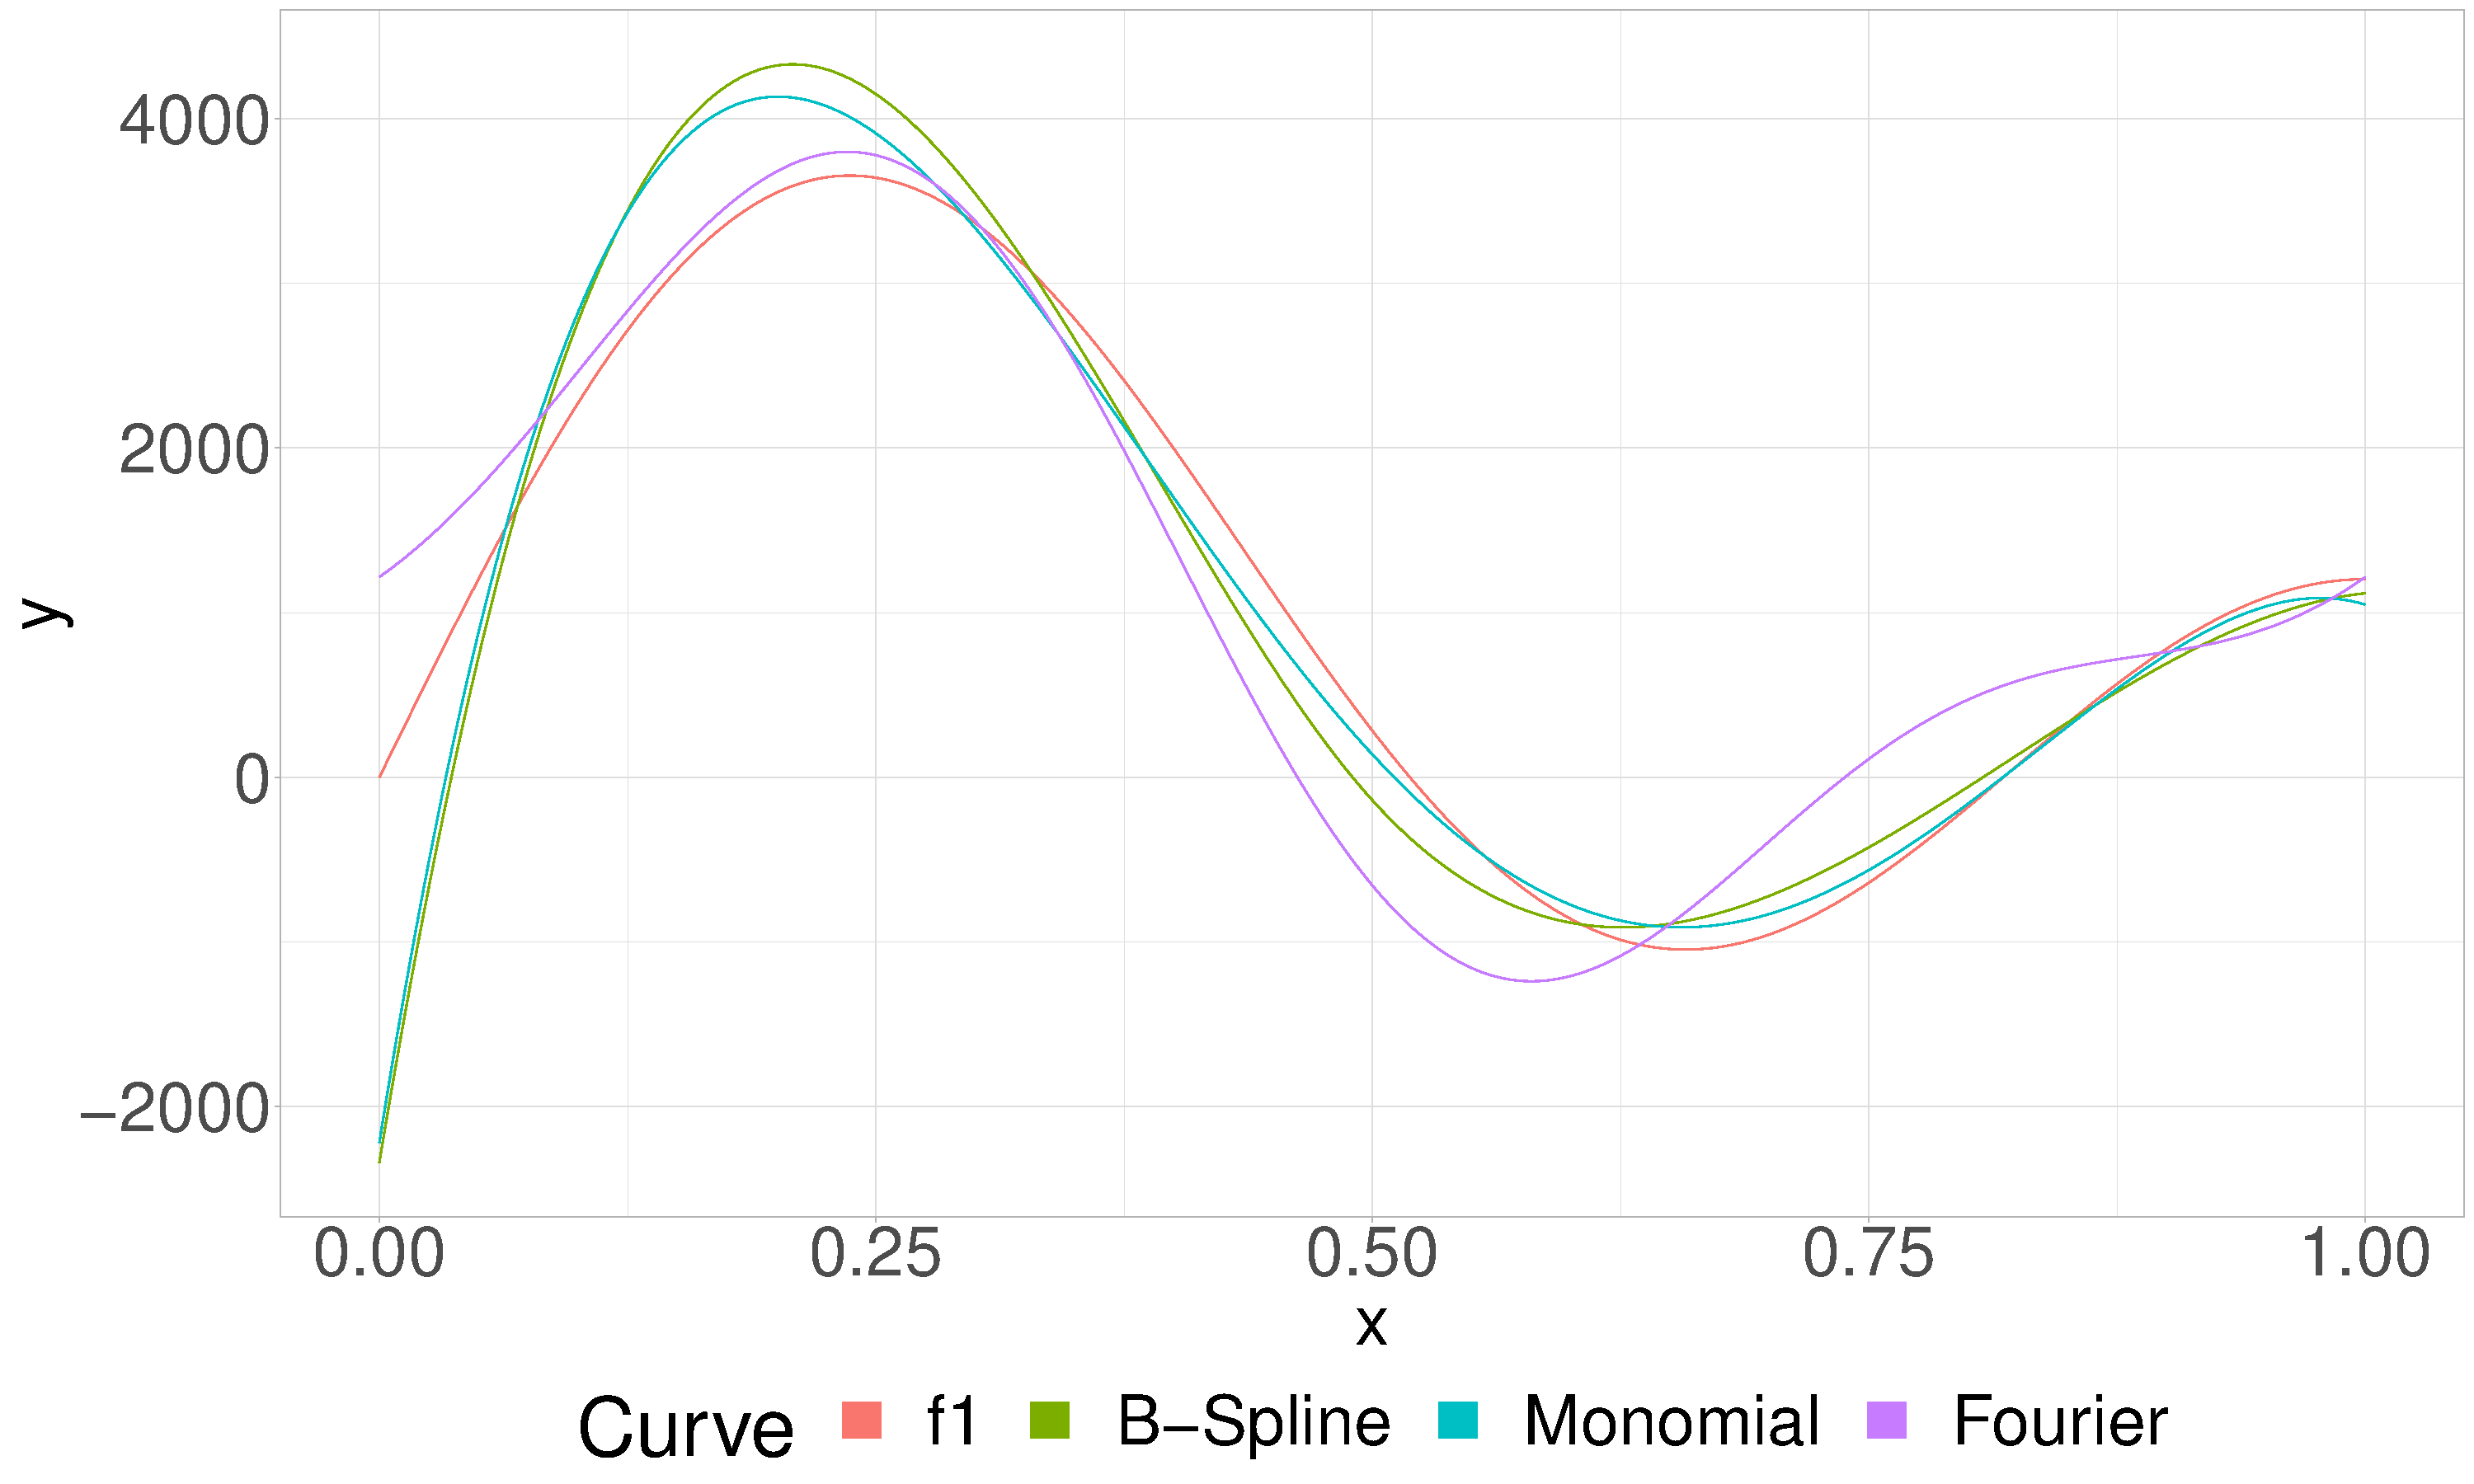
\includegraphics[width=\textwidth]{../Graphics/Curve\_Estimates/basis_expansion_1_1.pdf}
			\caption{Basis Expansion Regression - $f_1, Y_1$}
			\label{basis_expansion_1_1}
		\end{minipage}%
		\begin{minipage}{.5\textwidth}
			\centering
			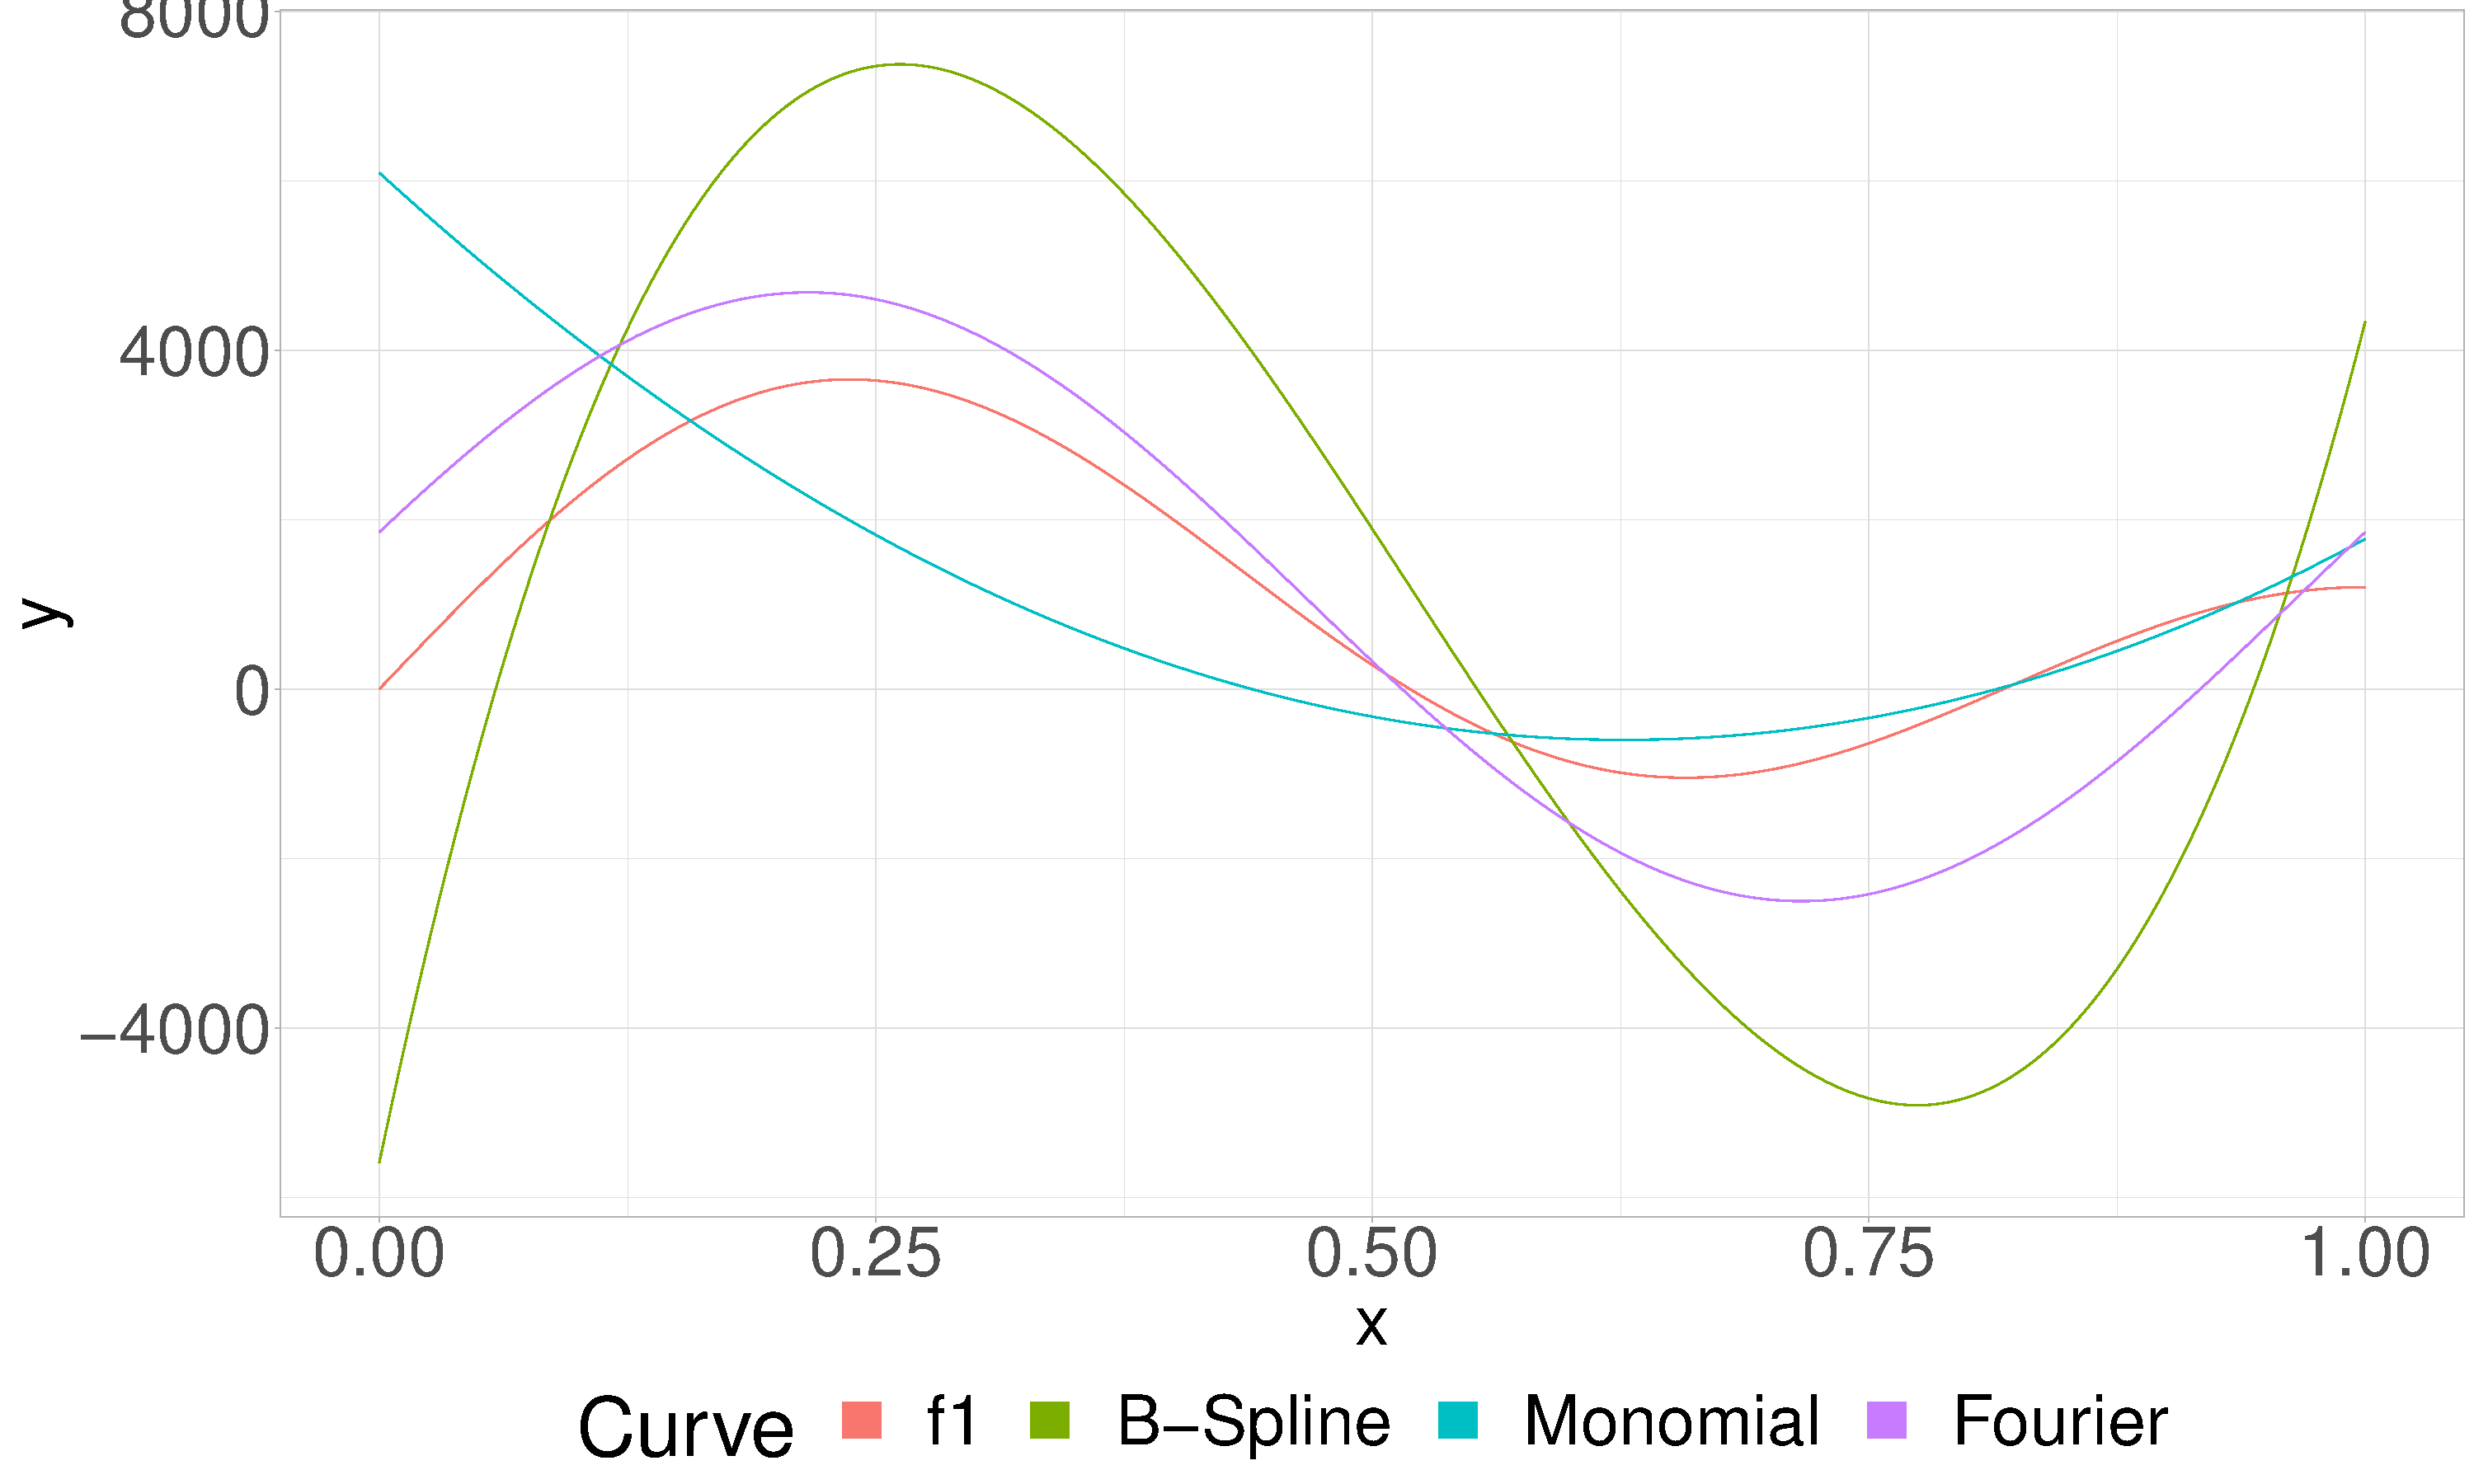
\includegraphics[width=\textwidth]{../Graphics/Curve\_Estimates/basis_expansion_1_2.pdf}
			\caption{Basis Expansion Regression - $f_1, Y_2$}
			\label{basis_expansion_1_2}
		\end{minipage}
	\end{figure}
	
	\begin{figure}[H]
		\centering
		\begin{minipage}{.5\textwidth}
			\centering
			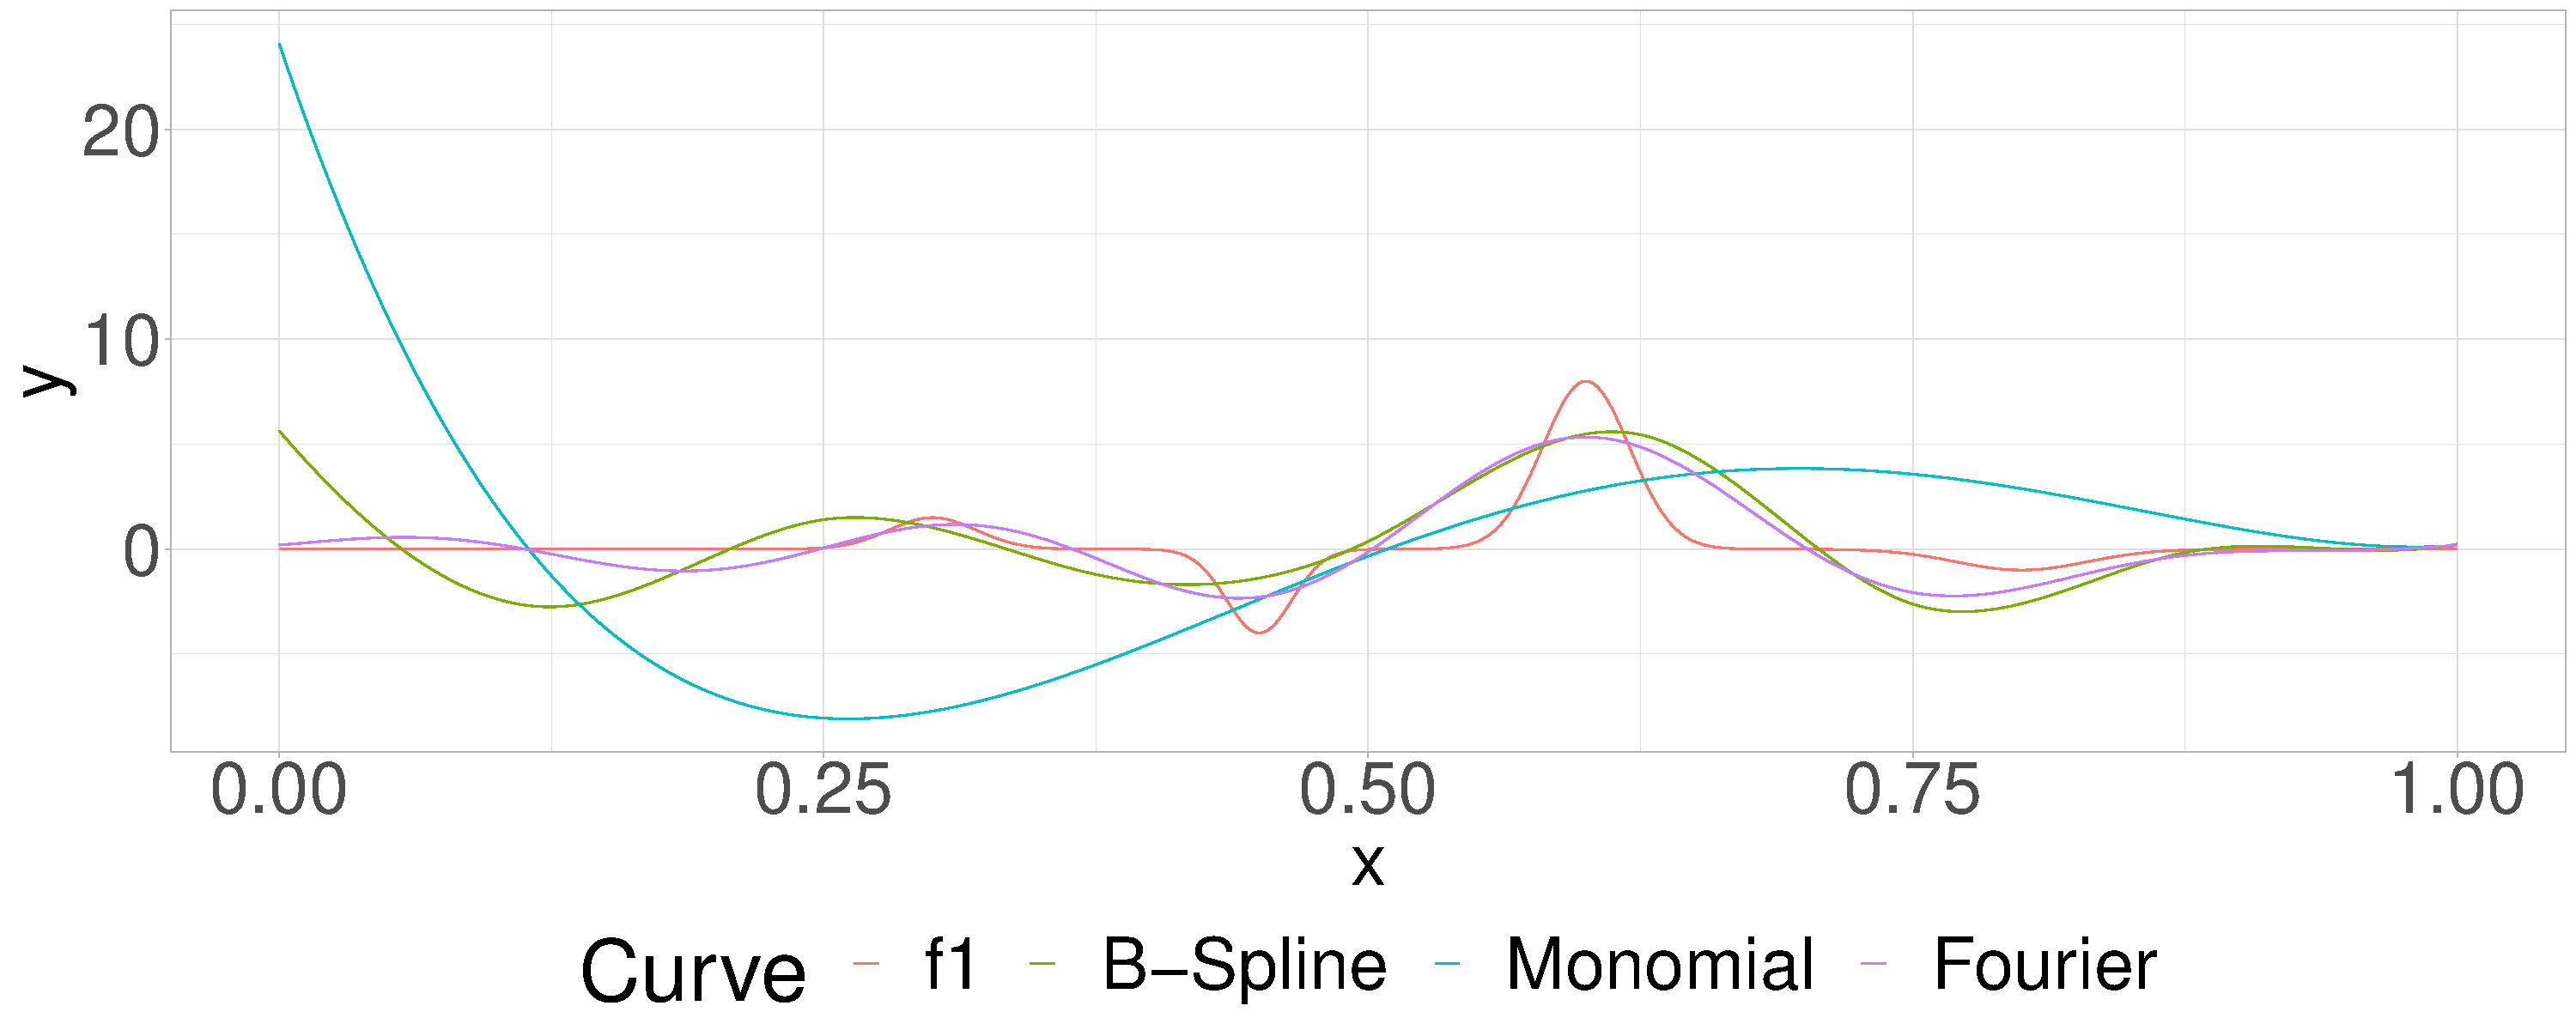
\includegraphics[width=\textwidth]{../Graphics/Curve\_Estimates/basis_expansion_2_1.pdf}
			\caption{Basis Expansion Regression - $f_2, Y_1$}
			\label{basis_expansion_2_1}
		\end{minipage}%
		\begin{minipage}{.5\textwidth}
			\centering
			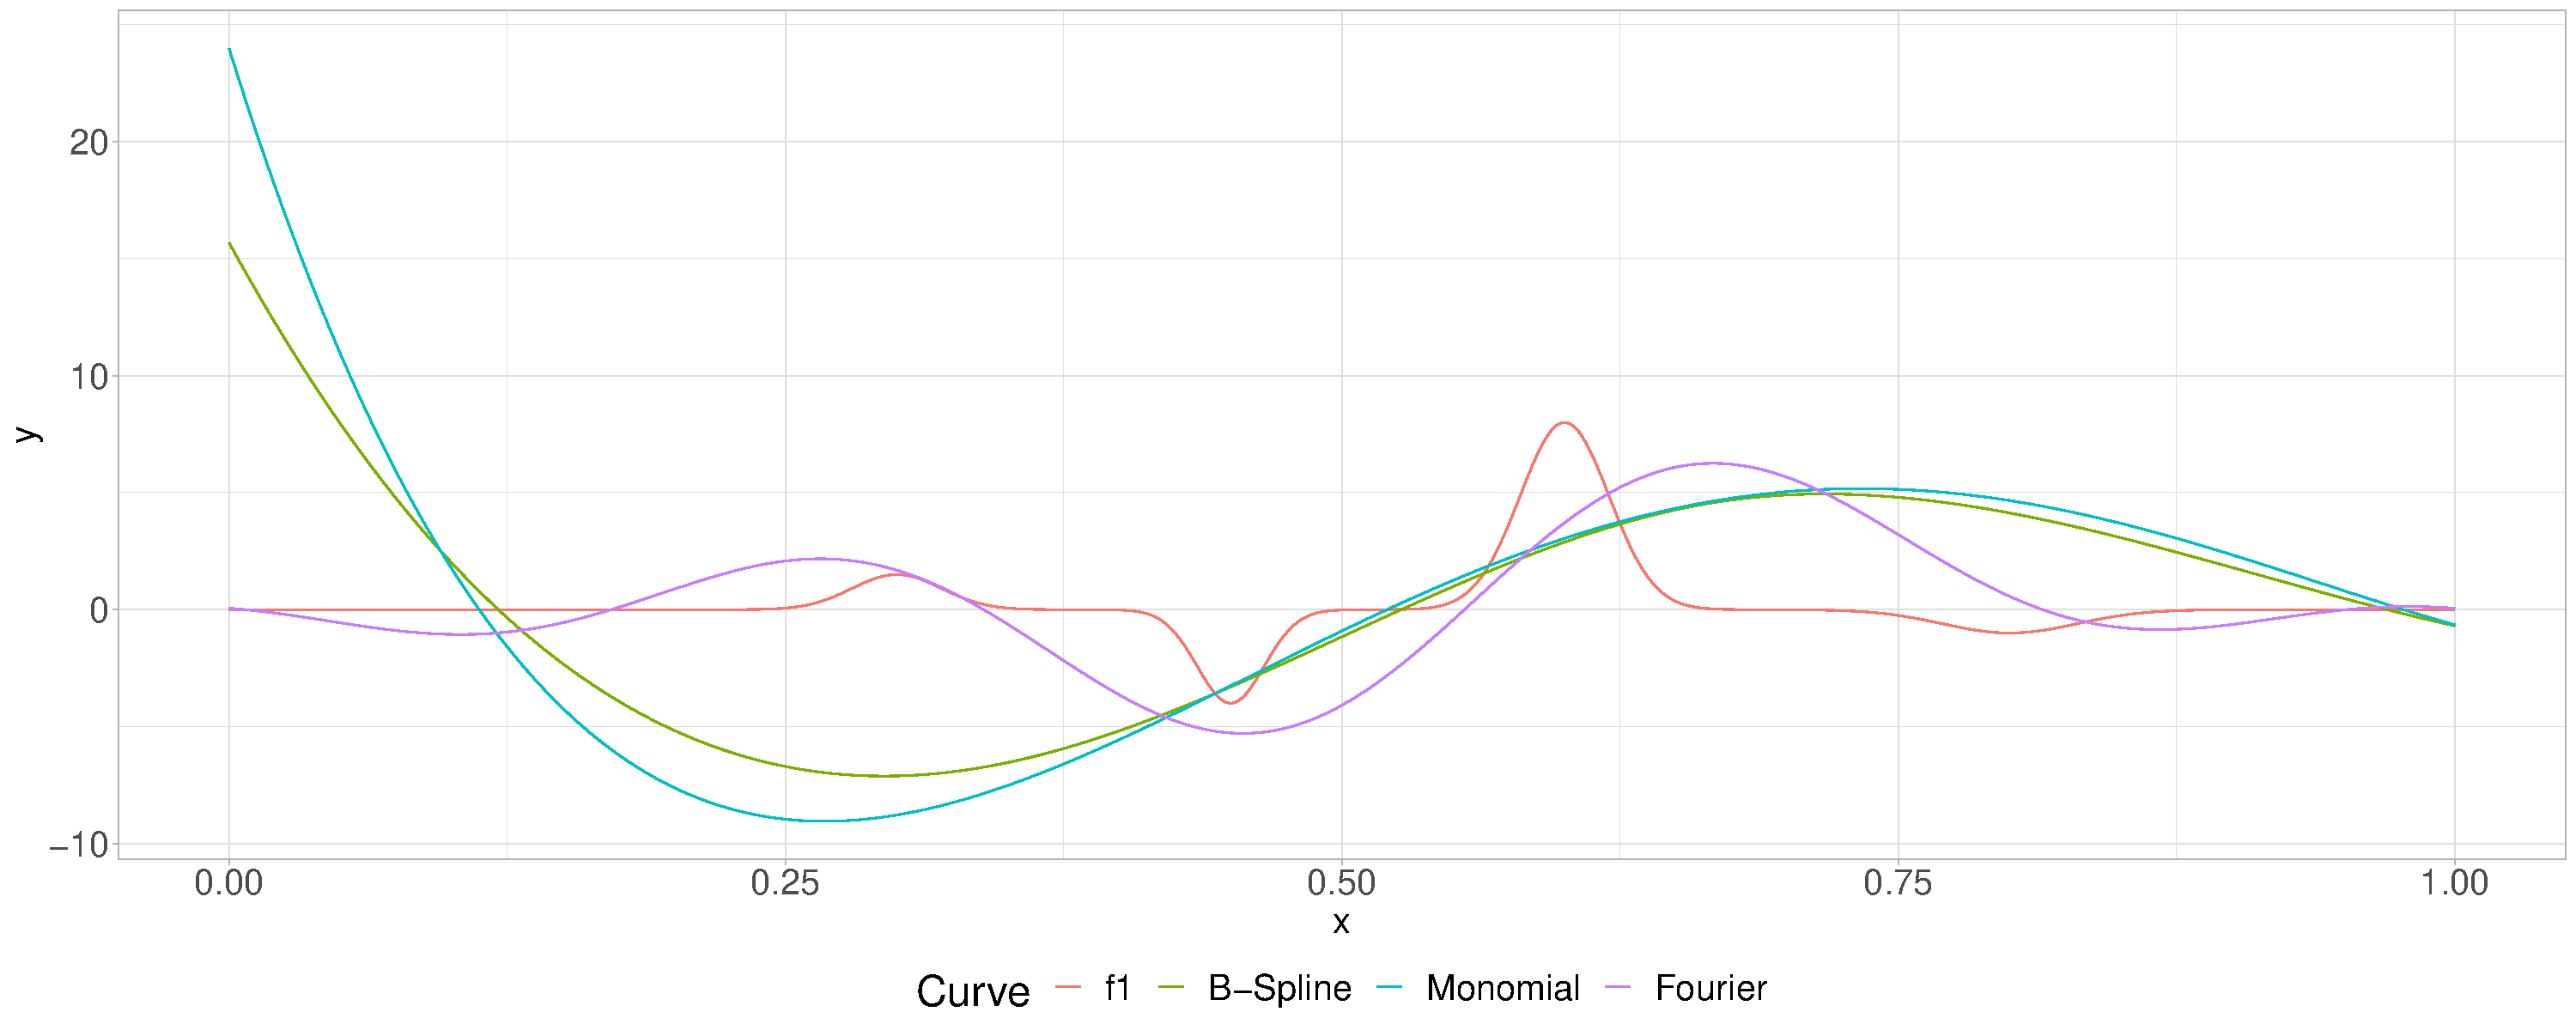
\includegraphics[width=\textwidth]{../Graphics/Curve\_Estimates/basis_expansion_2_2.pdf}
			\caption{Basis Expansion Regression - $f_2, Y_2$}
			\label{basis_expansion_2_2}
		\end{minipage}
	\end{figure}
	
	\begin{figure}[H]
		\centering
		\begin{minipage}{.5\textwidth}
			\centering
			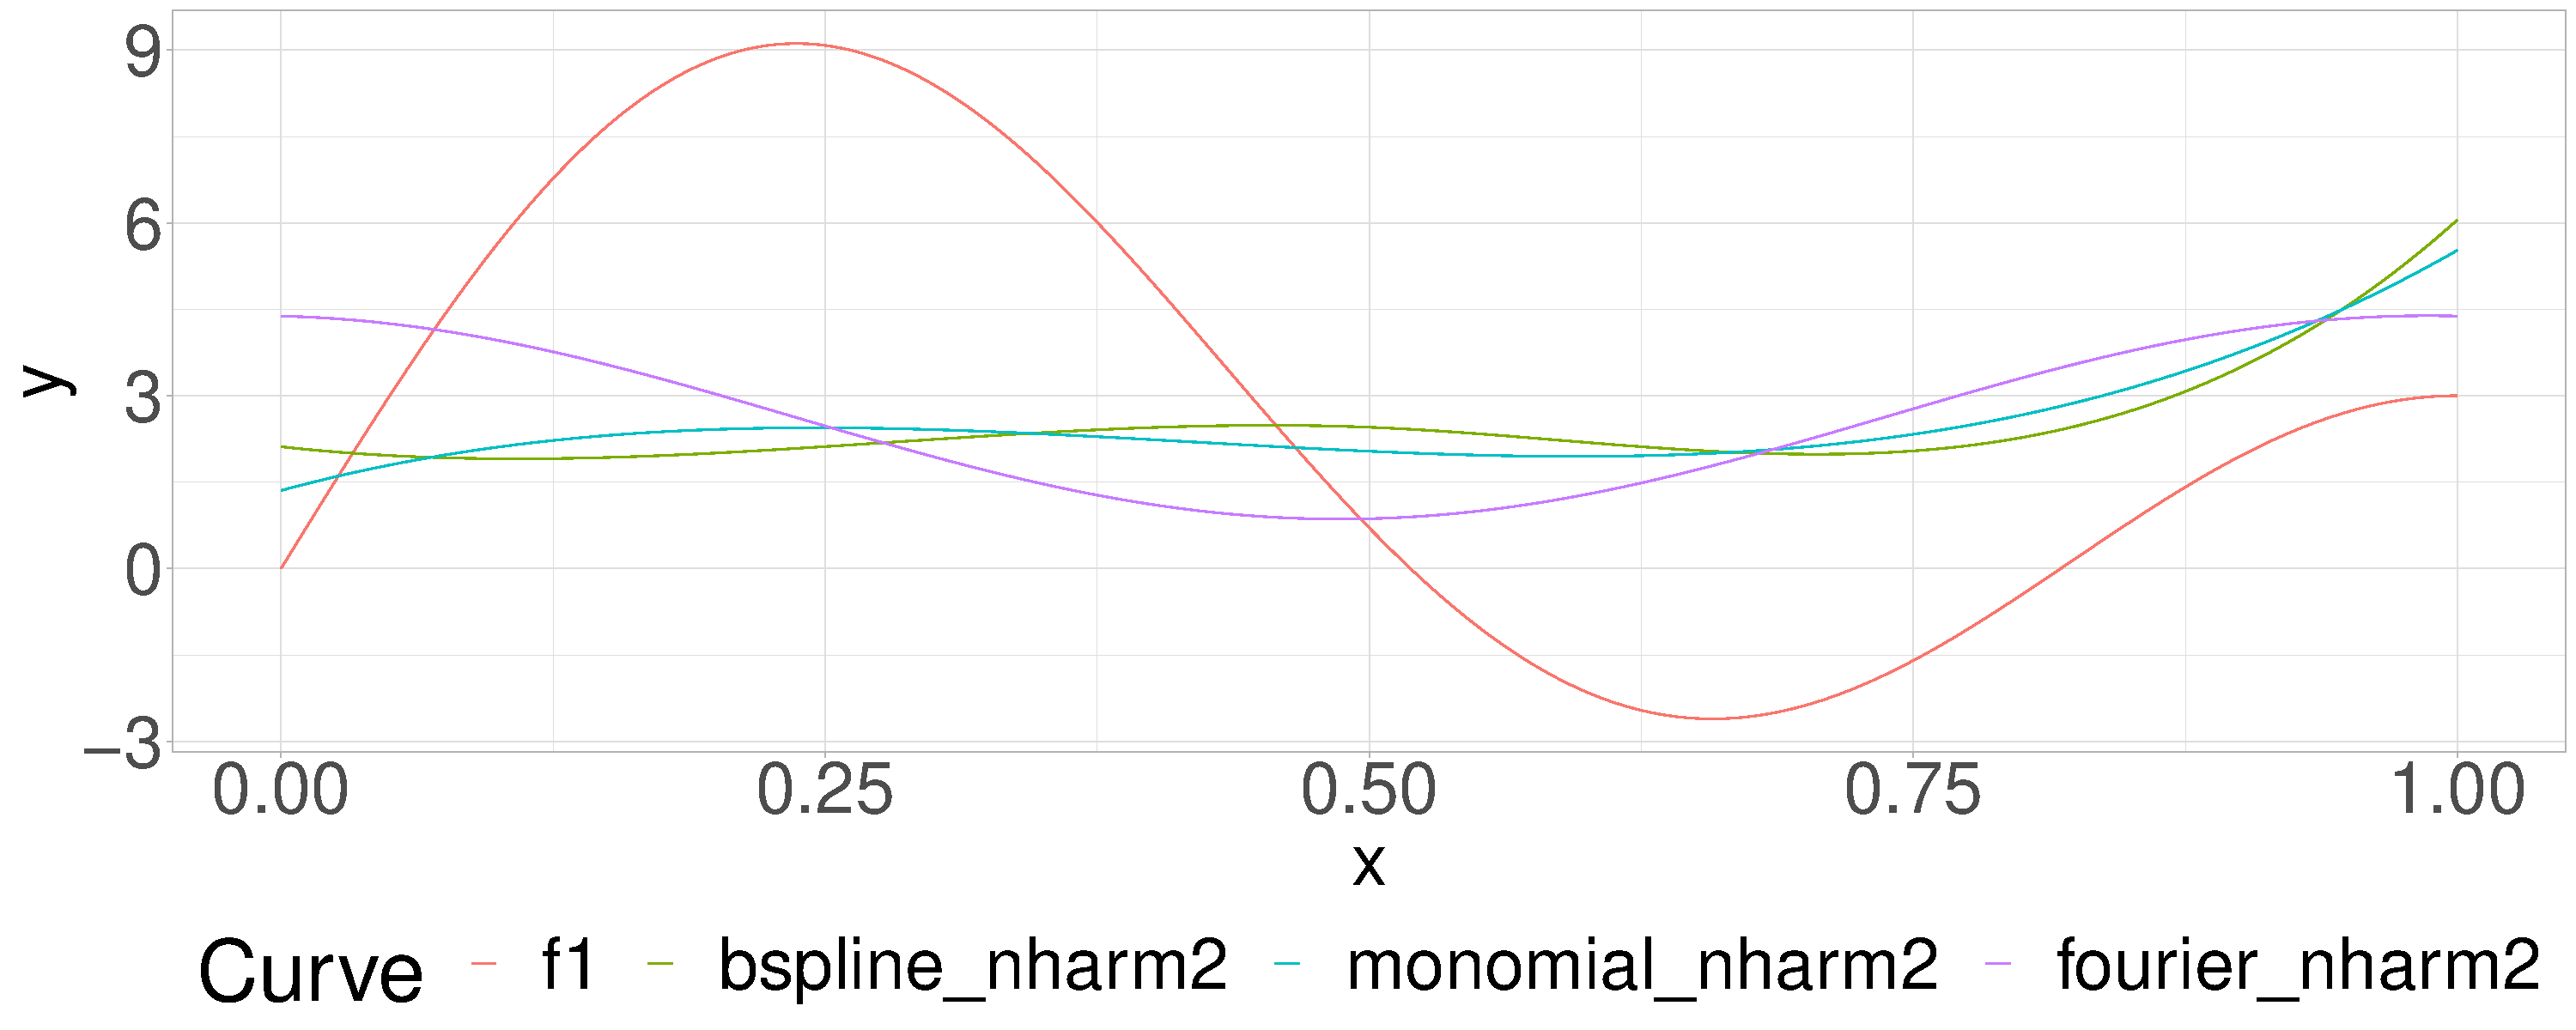
\includegraphics[width=\textwidth]{../Graphics/Curve\_Estimates/fpcr_nharm2_1_1.pdf}
			\caption{FPC Regression, 2 harmonics - $f_1, Y_1$}
			\label{fpcr_nharm2_1_1}
		\end{minipage}%
		\begin{minipage}{.5\textwidth}
			\centering
			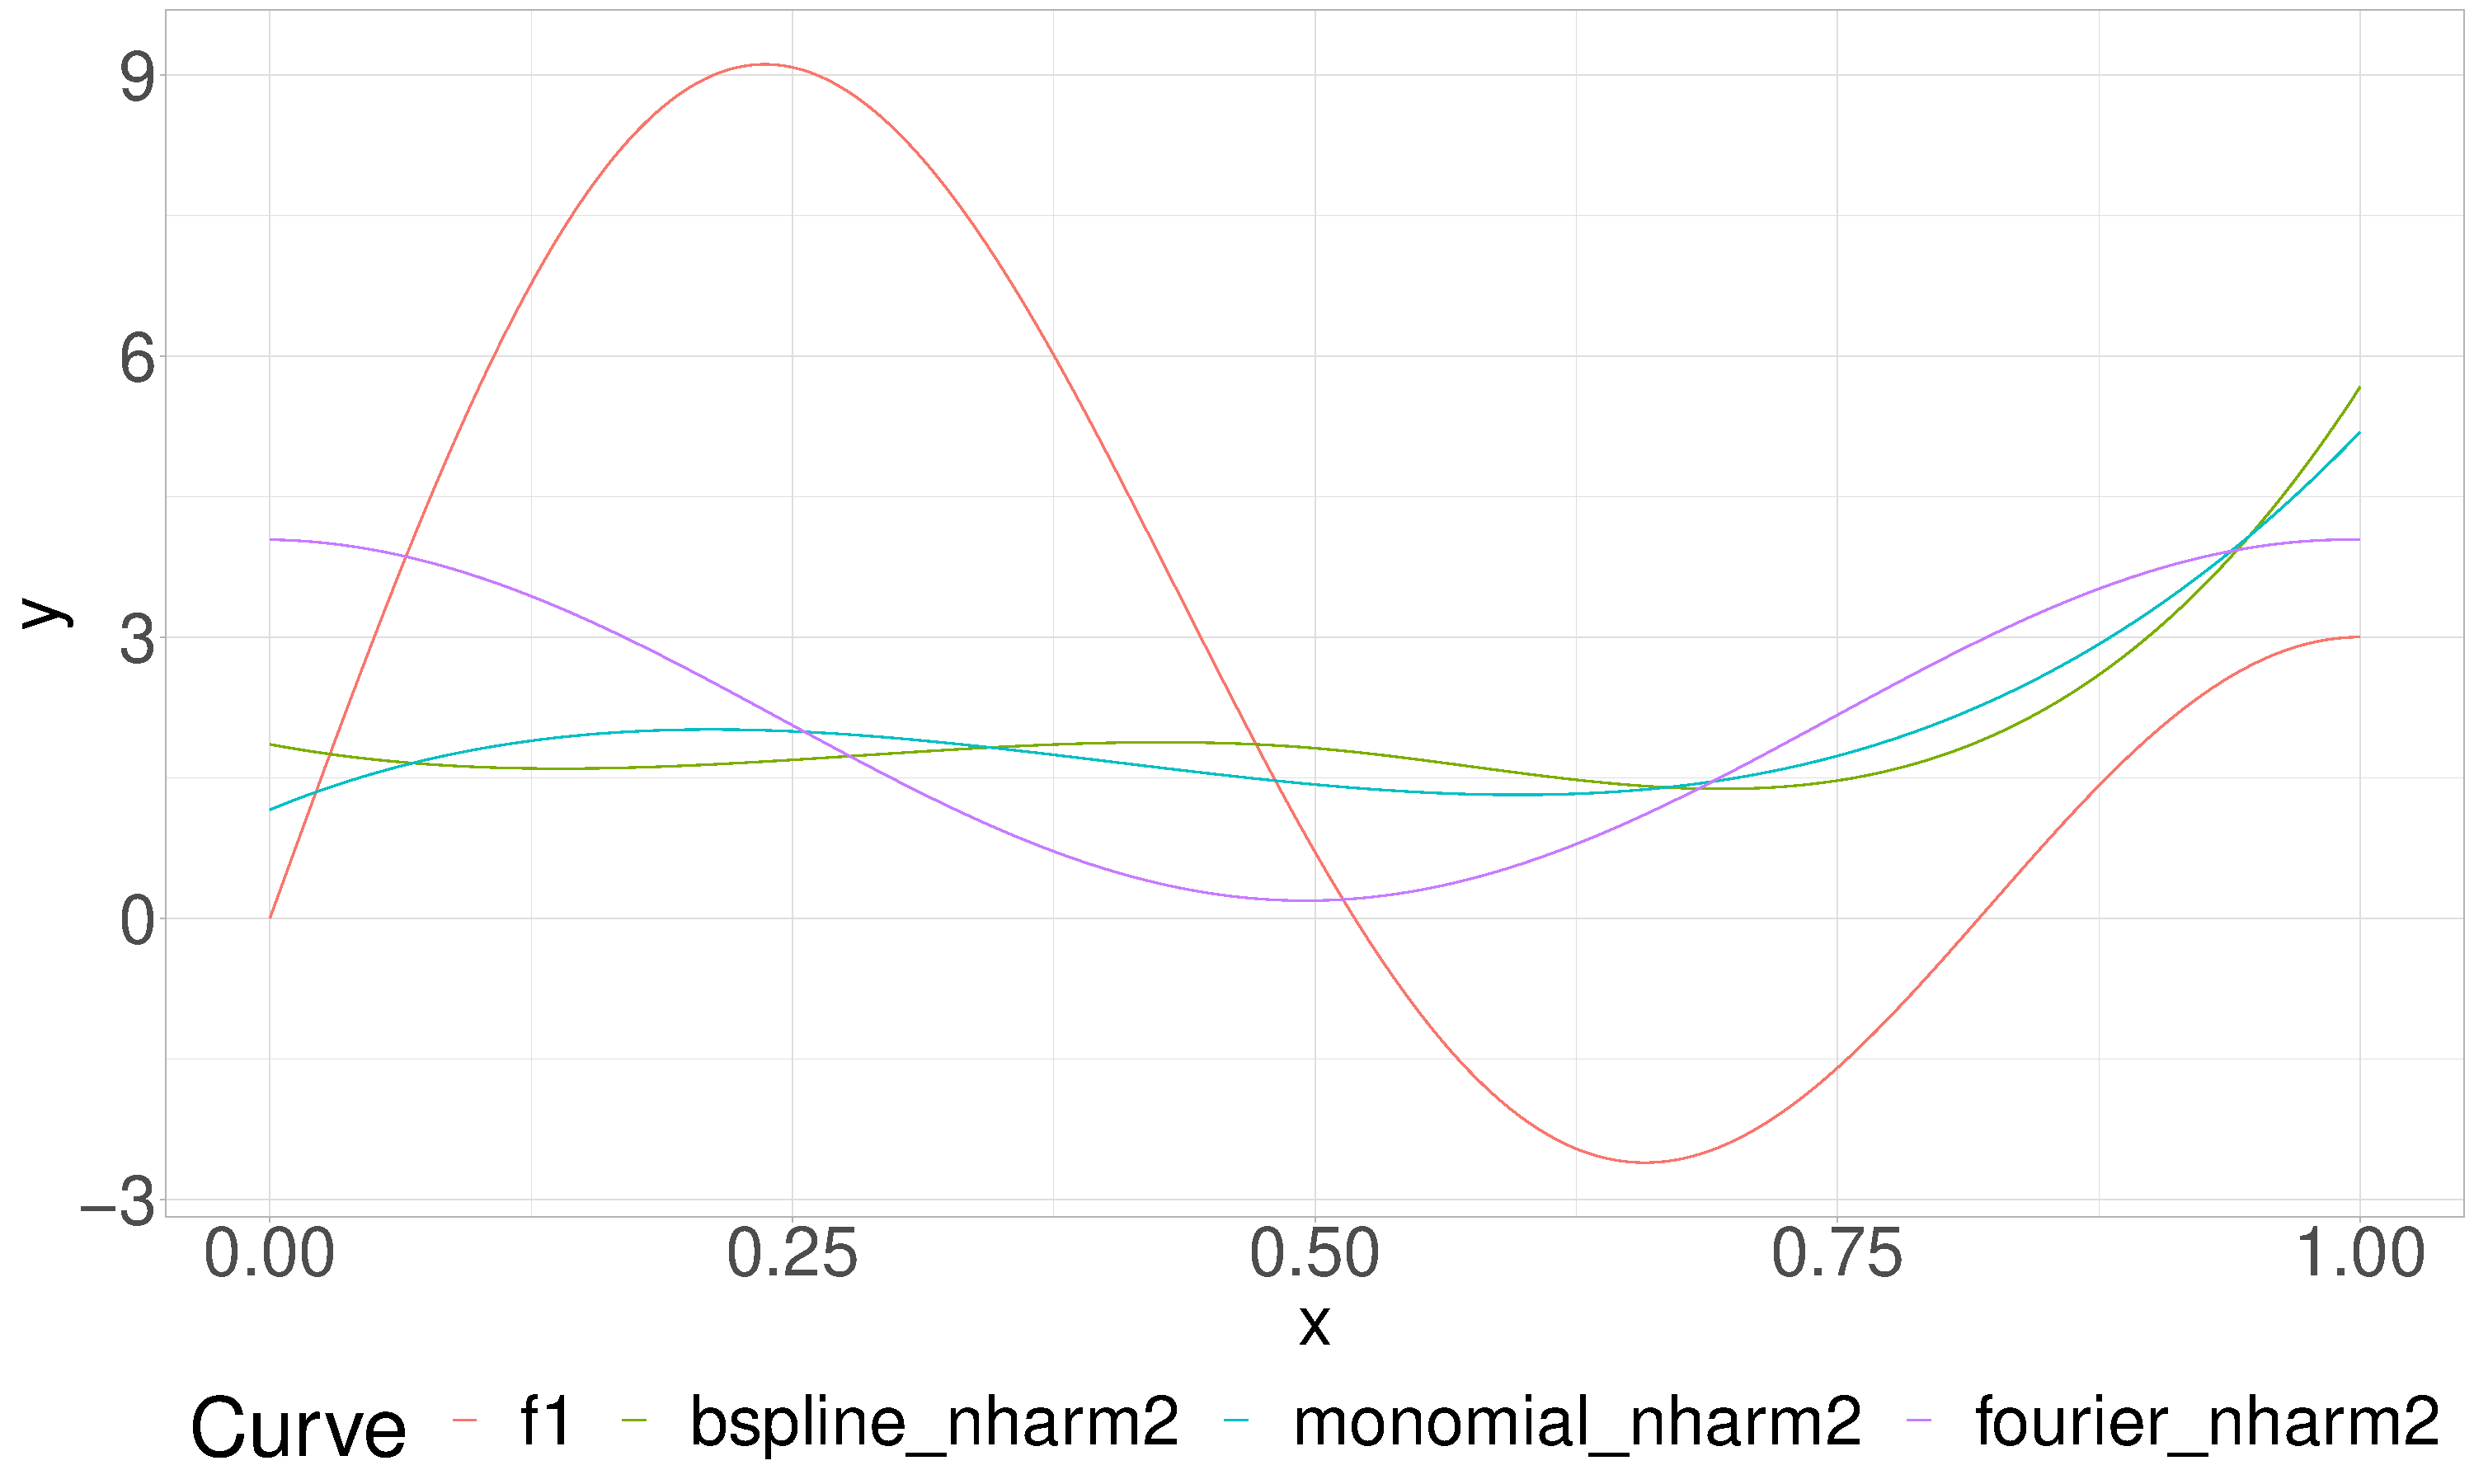
\includegraphics[width=\textwidth]{../Graphics/Curve\_Estimates/fpcr_nharm2_1_2.pdf}
			\caption{FPC Regression, 2 harmonics - $f_1, Y_2$}
			\label{fpcr_nharm2_1_2}
			
		\end{minipage}
	\end{figure}
	
	\begin{figure}[H]
		\centering
		\begin{minipage}{.5\textwidth}
			\centering
			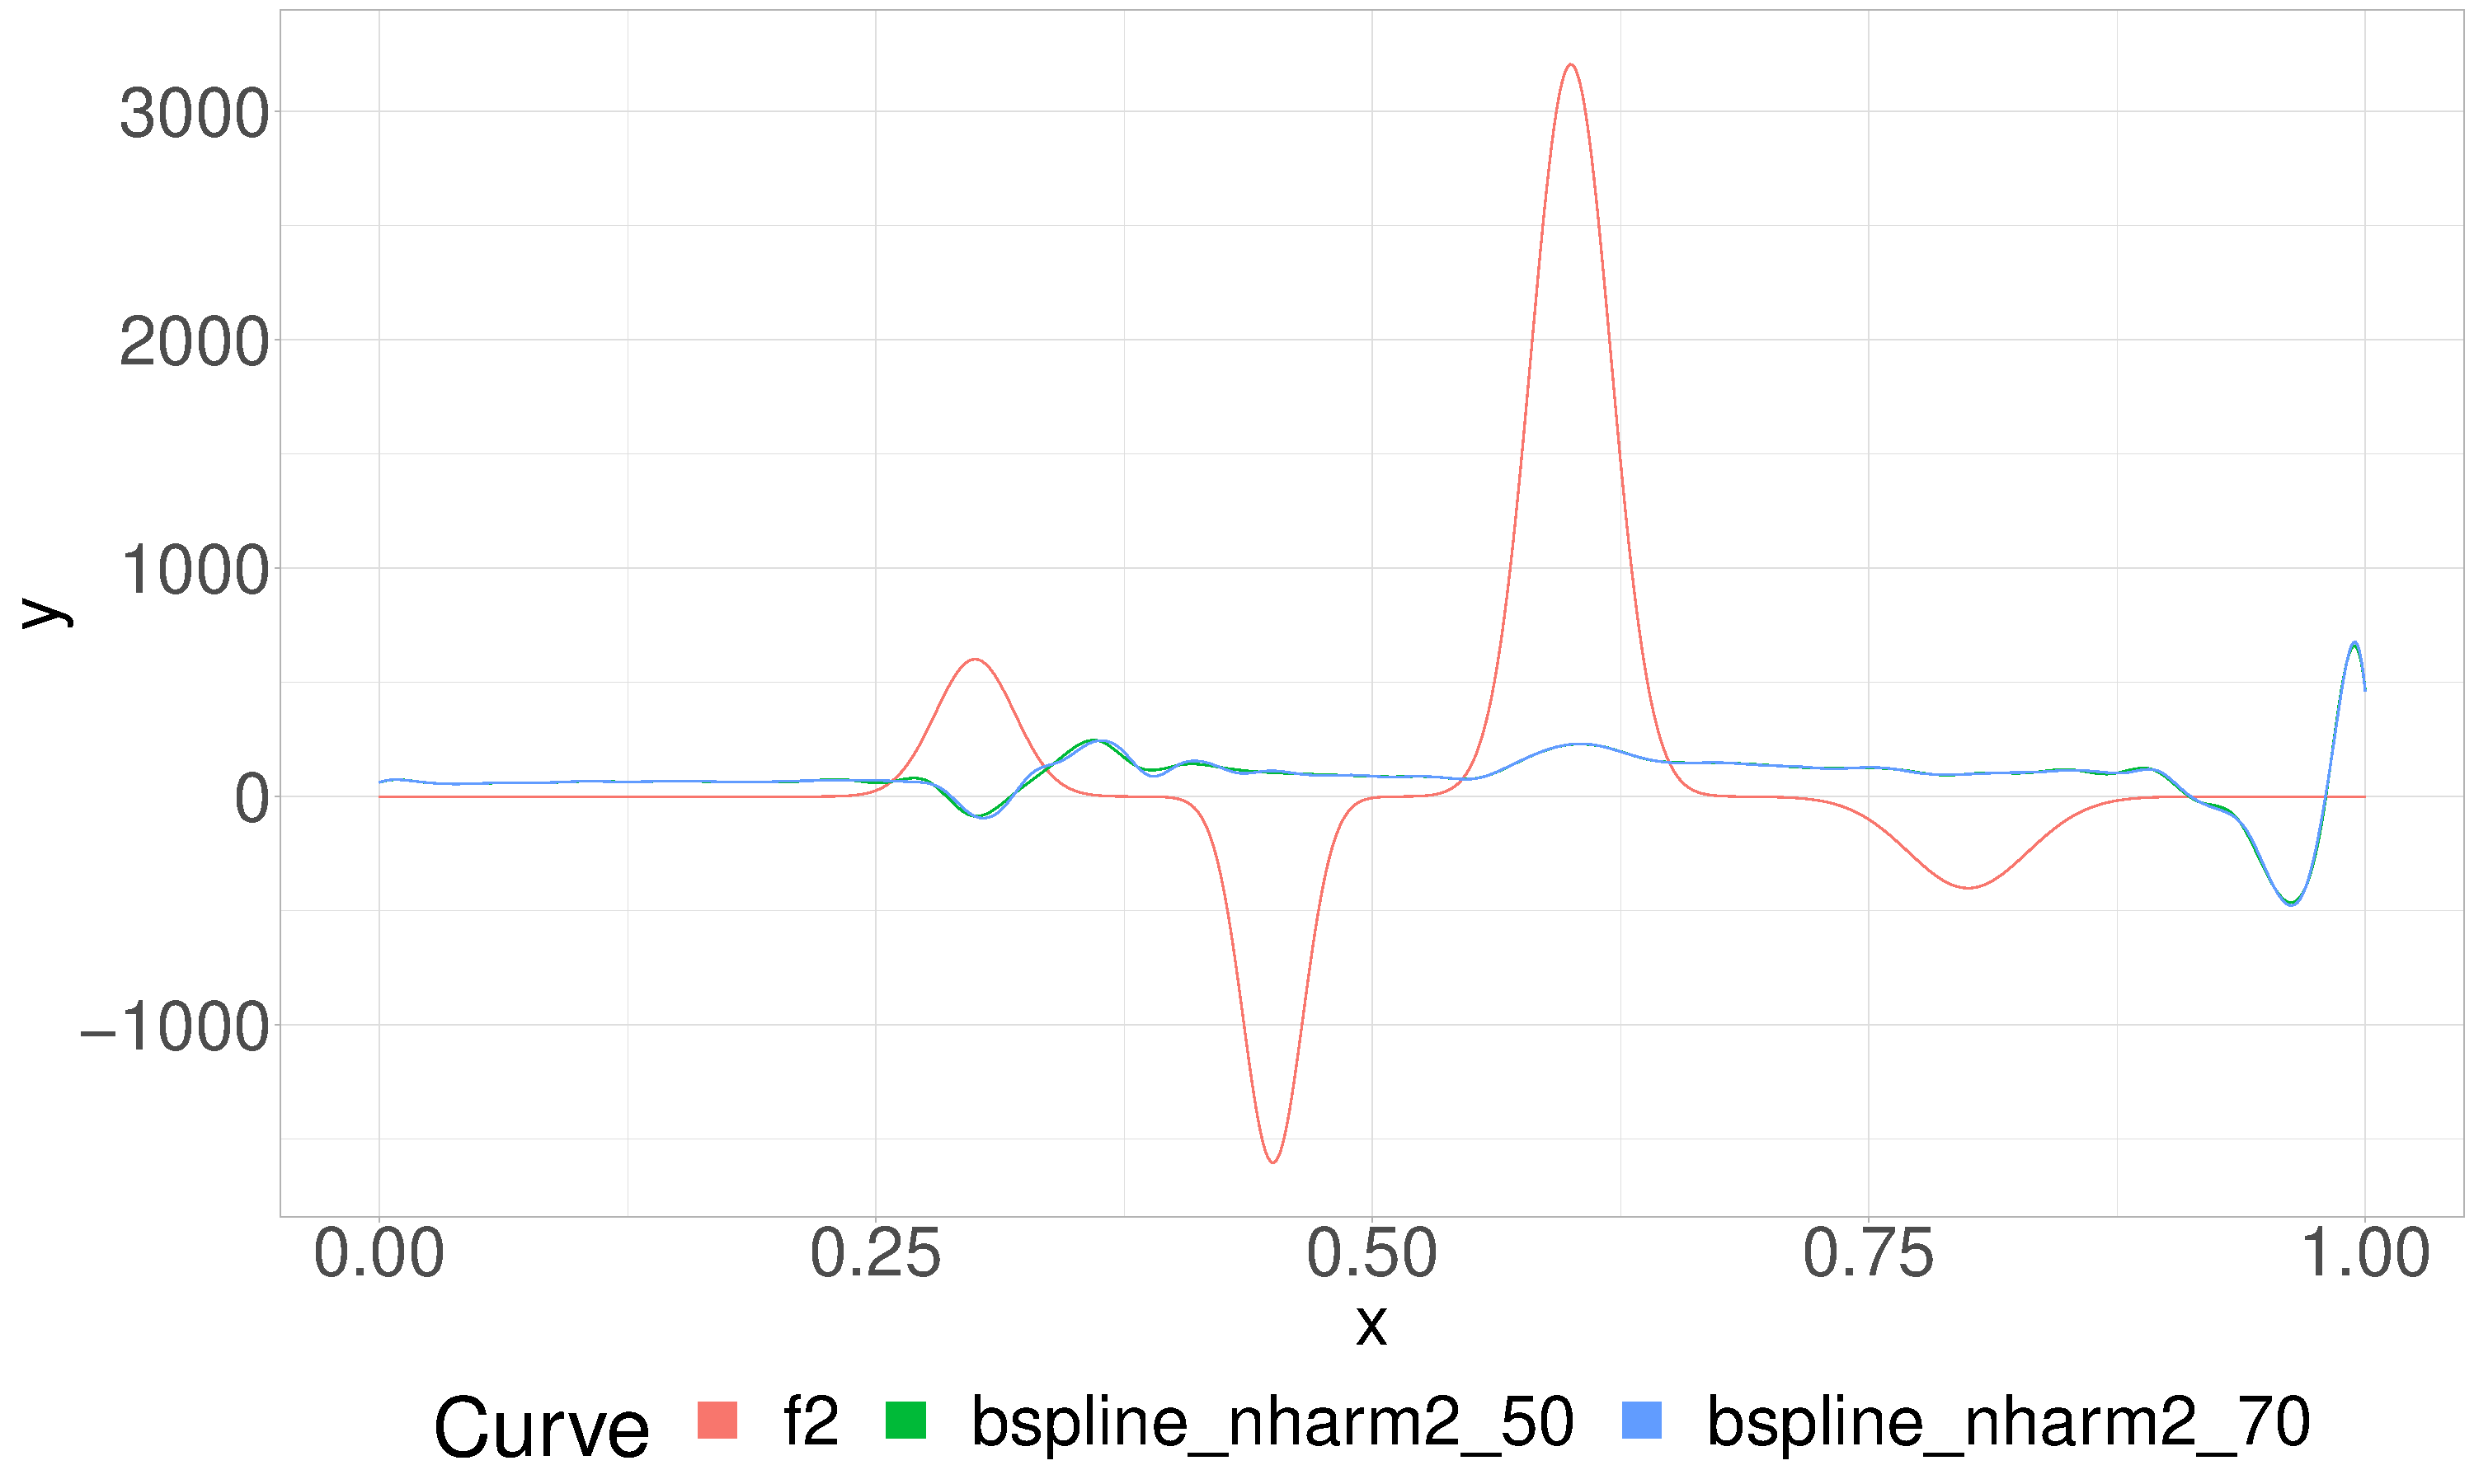
\includegraphics[width=\textwidth]{../Graphics/Curve\_Estimates/fpcr_nharm2_2_1.pdf}
			\caption{FPC Regression, 2 harmonics - $f_2, Y_1$}
			\label{fpcr_nharm2_2_1}
		\end{minipage}%
		\begin{minipage}{.5\textwidth}
			\centering
			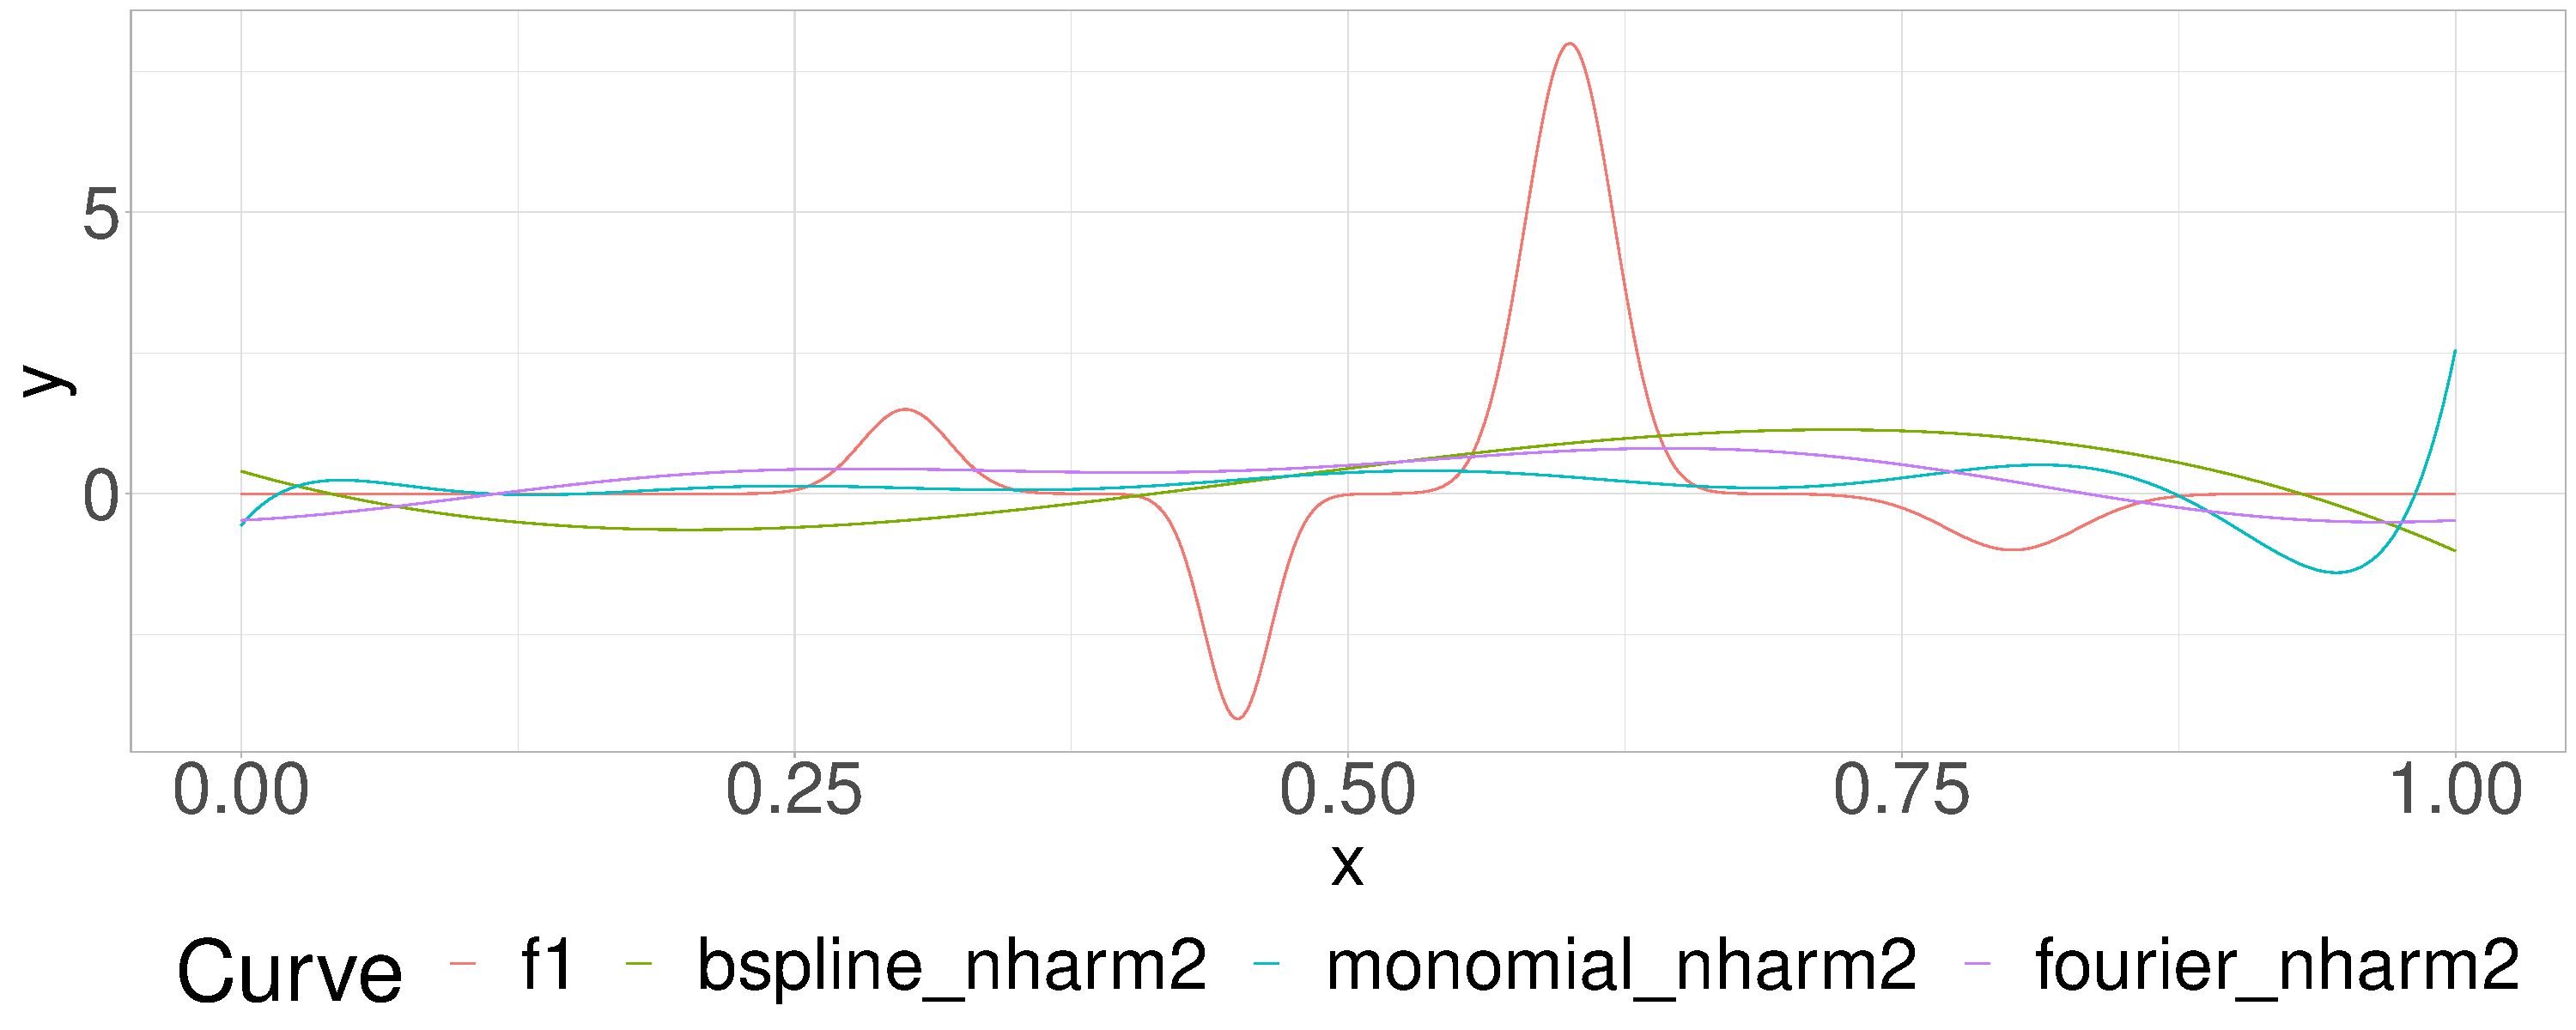
\includegraphics[width=\textwidth]{../Graphics/Curve\_Estimates/fpcr_nharm2_2_2.pdf}
			\caption{FPC Regression, 2 harmonics - $f_2, Y_2$}
			\label{fpcr_nharm2_2_2}
		\end{minipage}
	\end{figure}
	
	\begin{figure}[H]
		\centering
		\begin{minipage}{.5\textwidth}
			\centering
			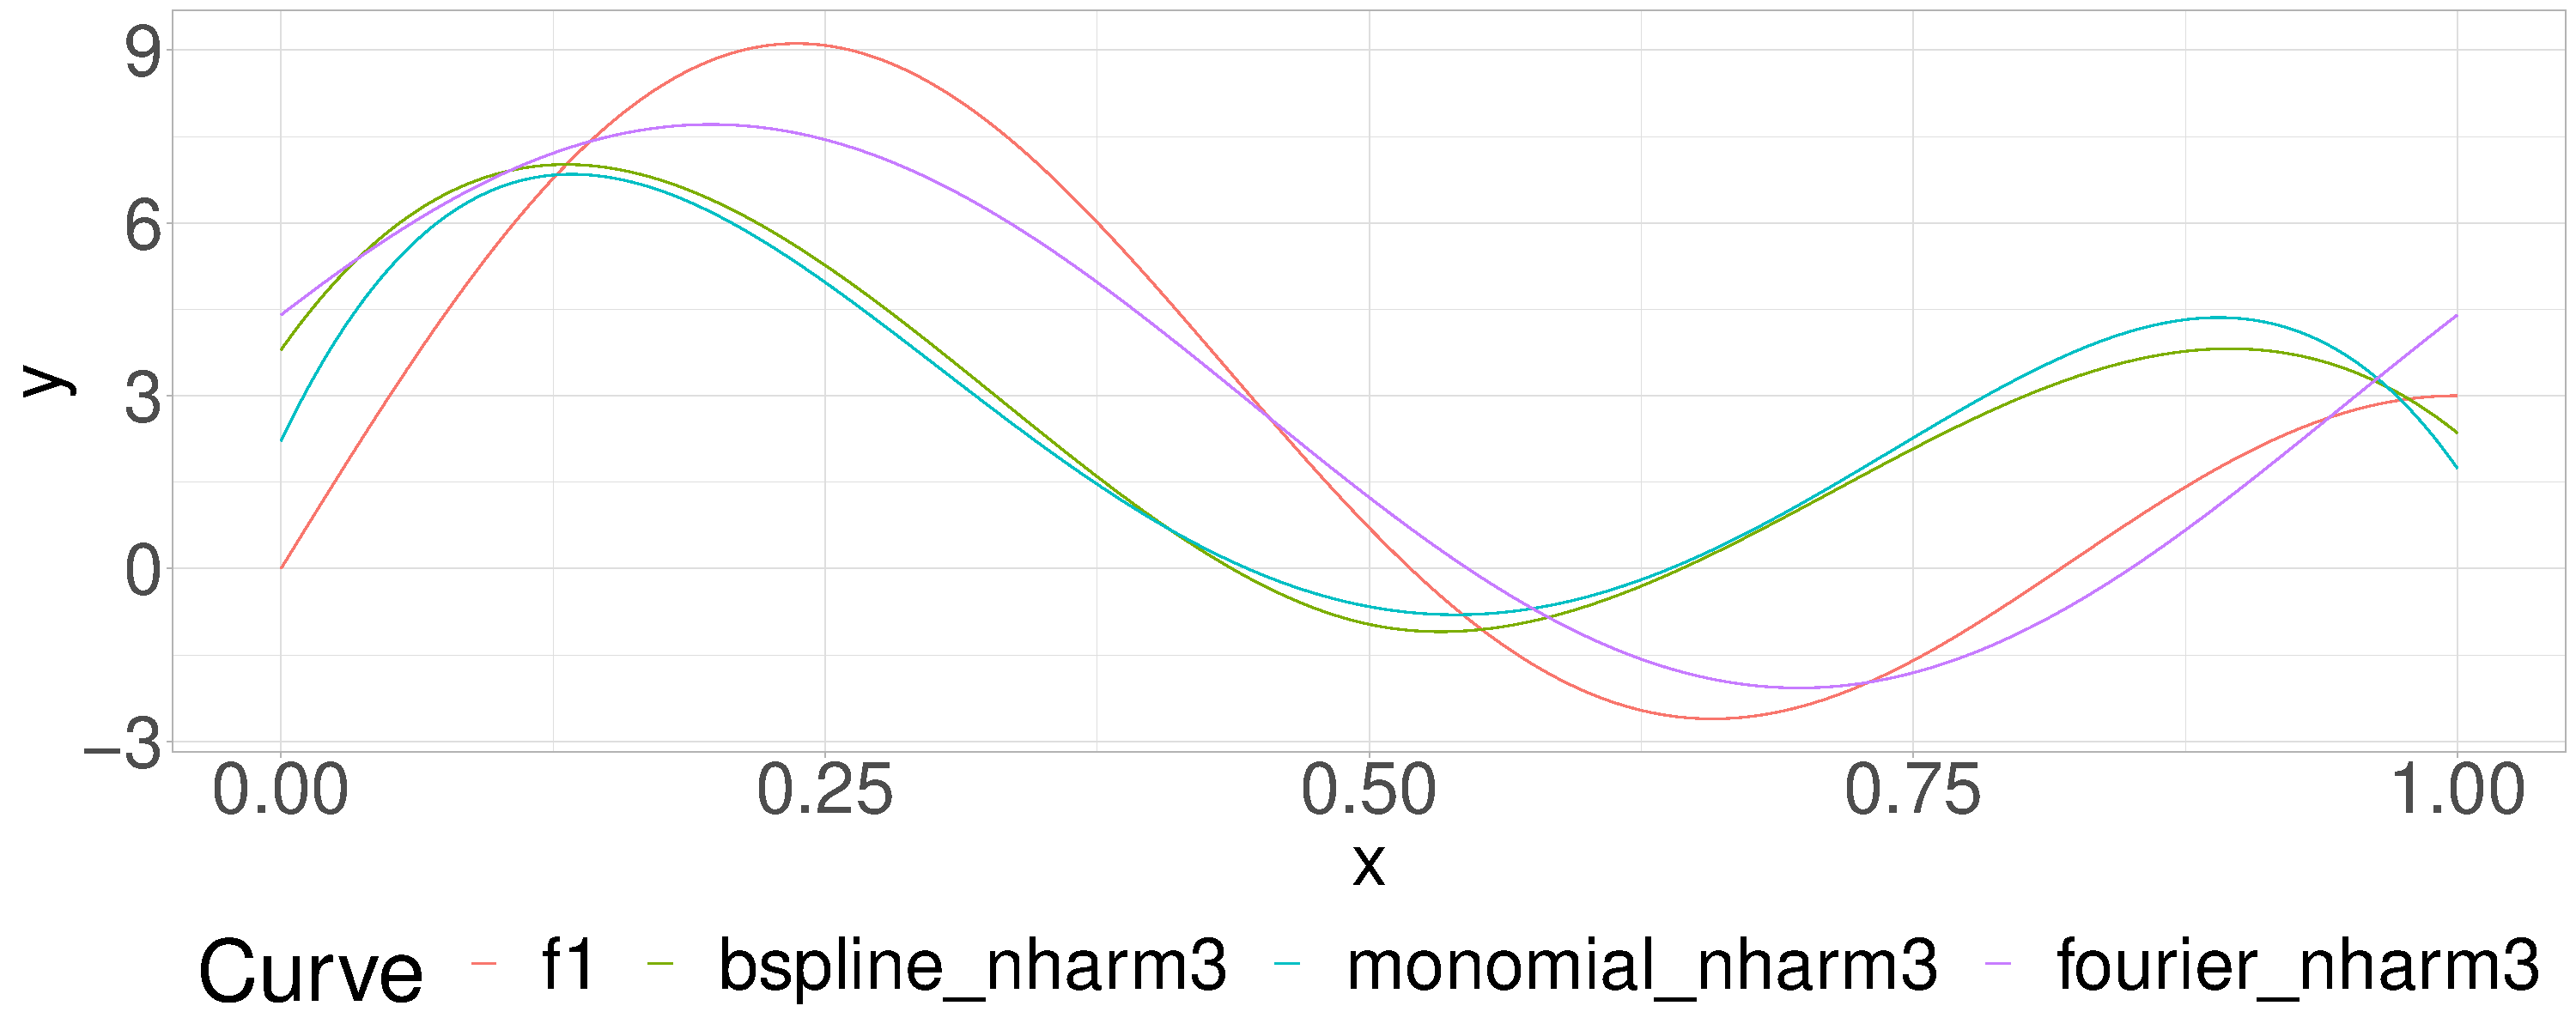
\includegraphics[width=\textwidth]{../Graphics/Curve\_Estimates/fpcr_nharm3_1_1.pdf}
			\caption{FPC Regression, 3 harmonics - $f_1, Y_1$}
			\label{fpcr_nharm3_1_1}
		\end{minipage}%
		\begin{minipage}{.5\textwidth}
			\centering
			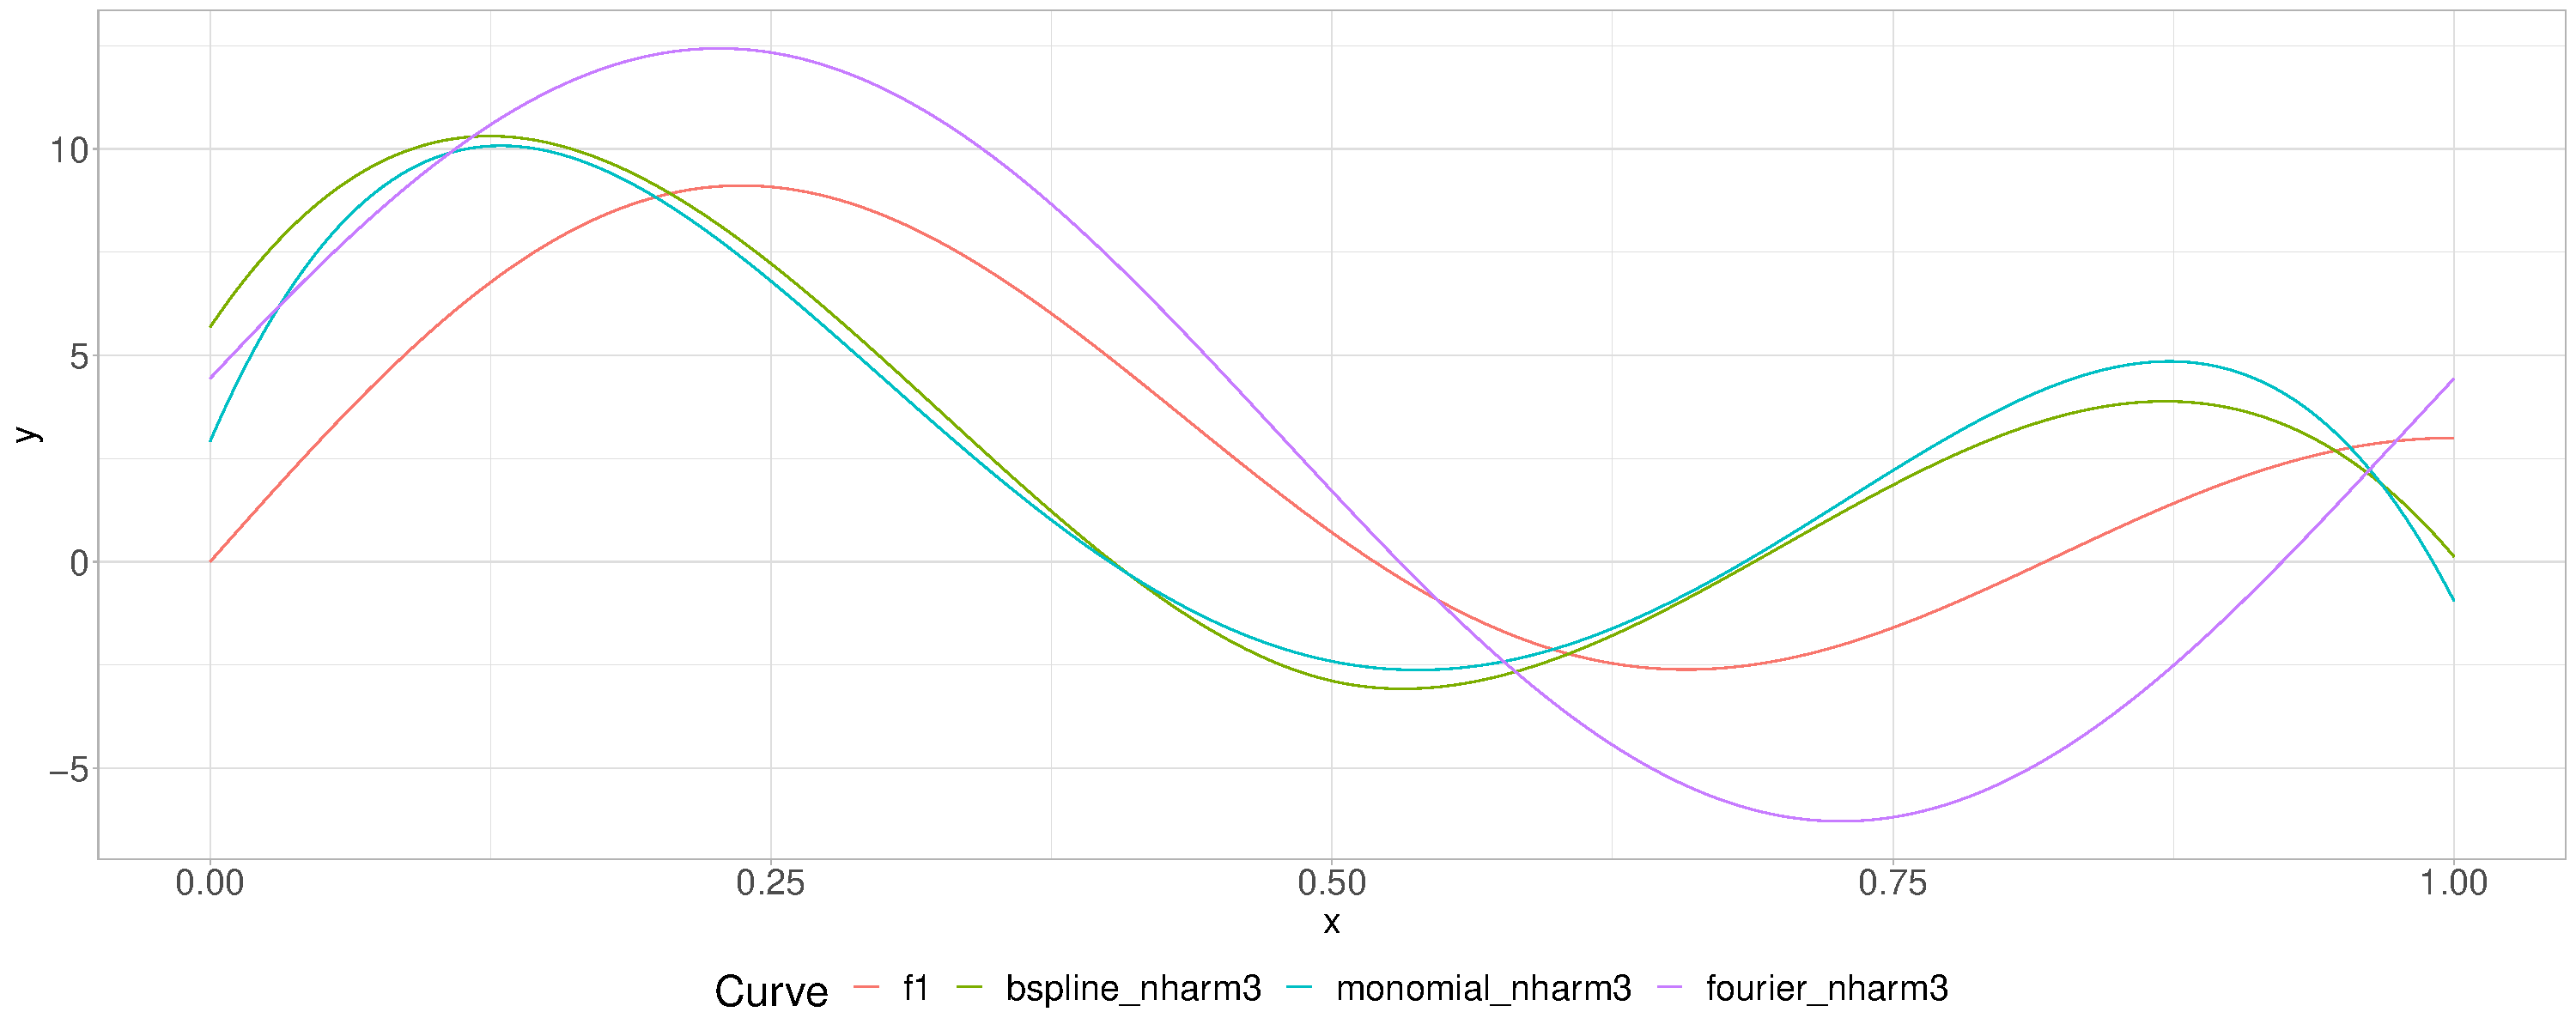
\includegraphics[width=\textwidth]{../Graphics/Curve\_Estimates/fpcr_nharm3_1_2.pdf}
			\caption{FPC Regression, 3 harmonics - $f_1, Y_2$}
			\label{fpcr_nharm3_1_2}
		\end{minipage}
	\end{figure}
	
	\begin{figure}[H]
		\centering
		\begin{minipage}{.5\textwidth}
			\centering
			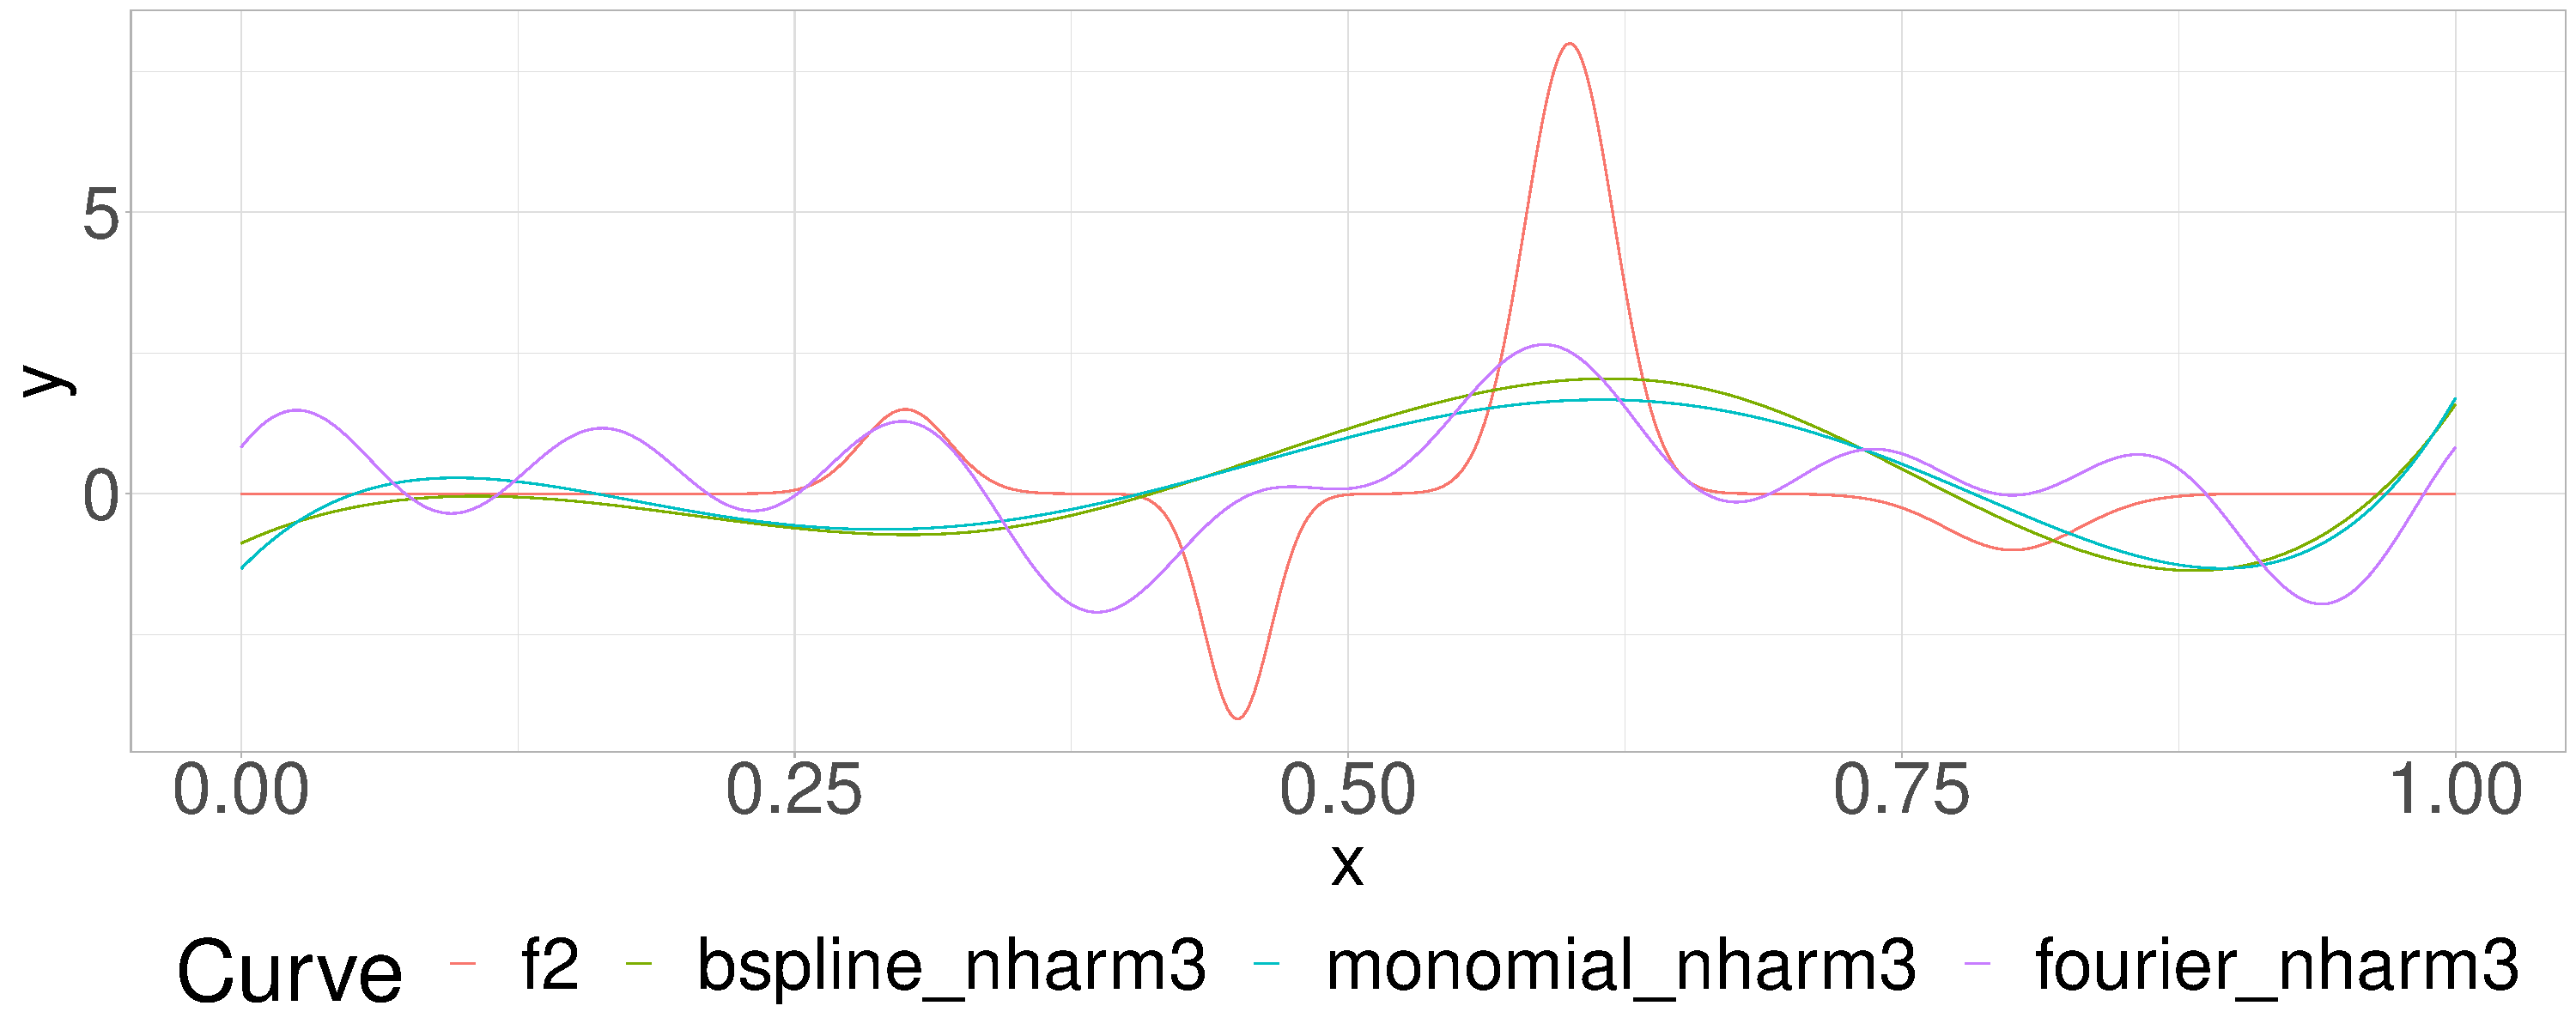
\includegraphics[width=\textwidth]{../Graphics/Curve\_Estimates/fpcr_nharm3_2_1.pdf}
			\caption{FPC Regression, 3 harmonics - $f_2, Y_1$}
			\label{fpcr_nharm3_2_1}
		\end{minipage}%
		\begin{minipage}{.5\textwidth}
			\centering
			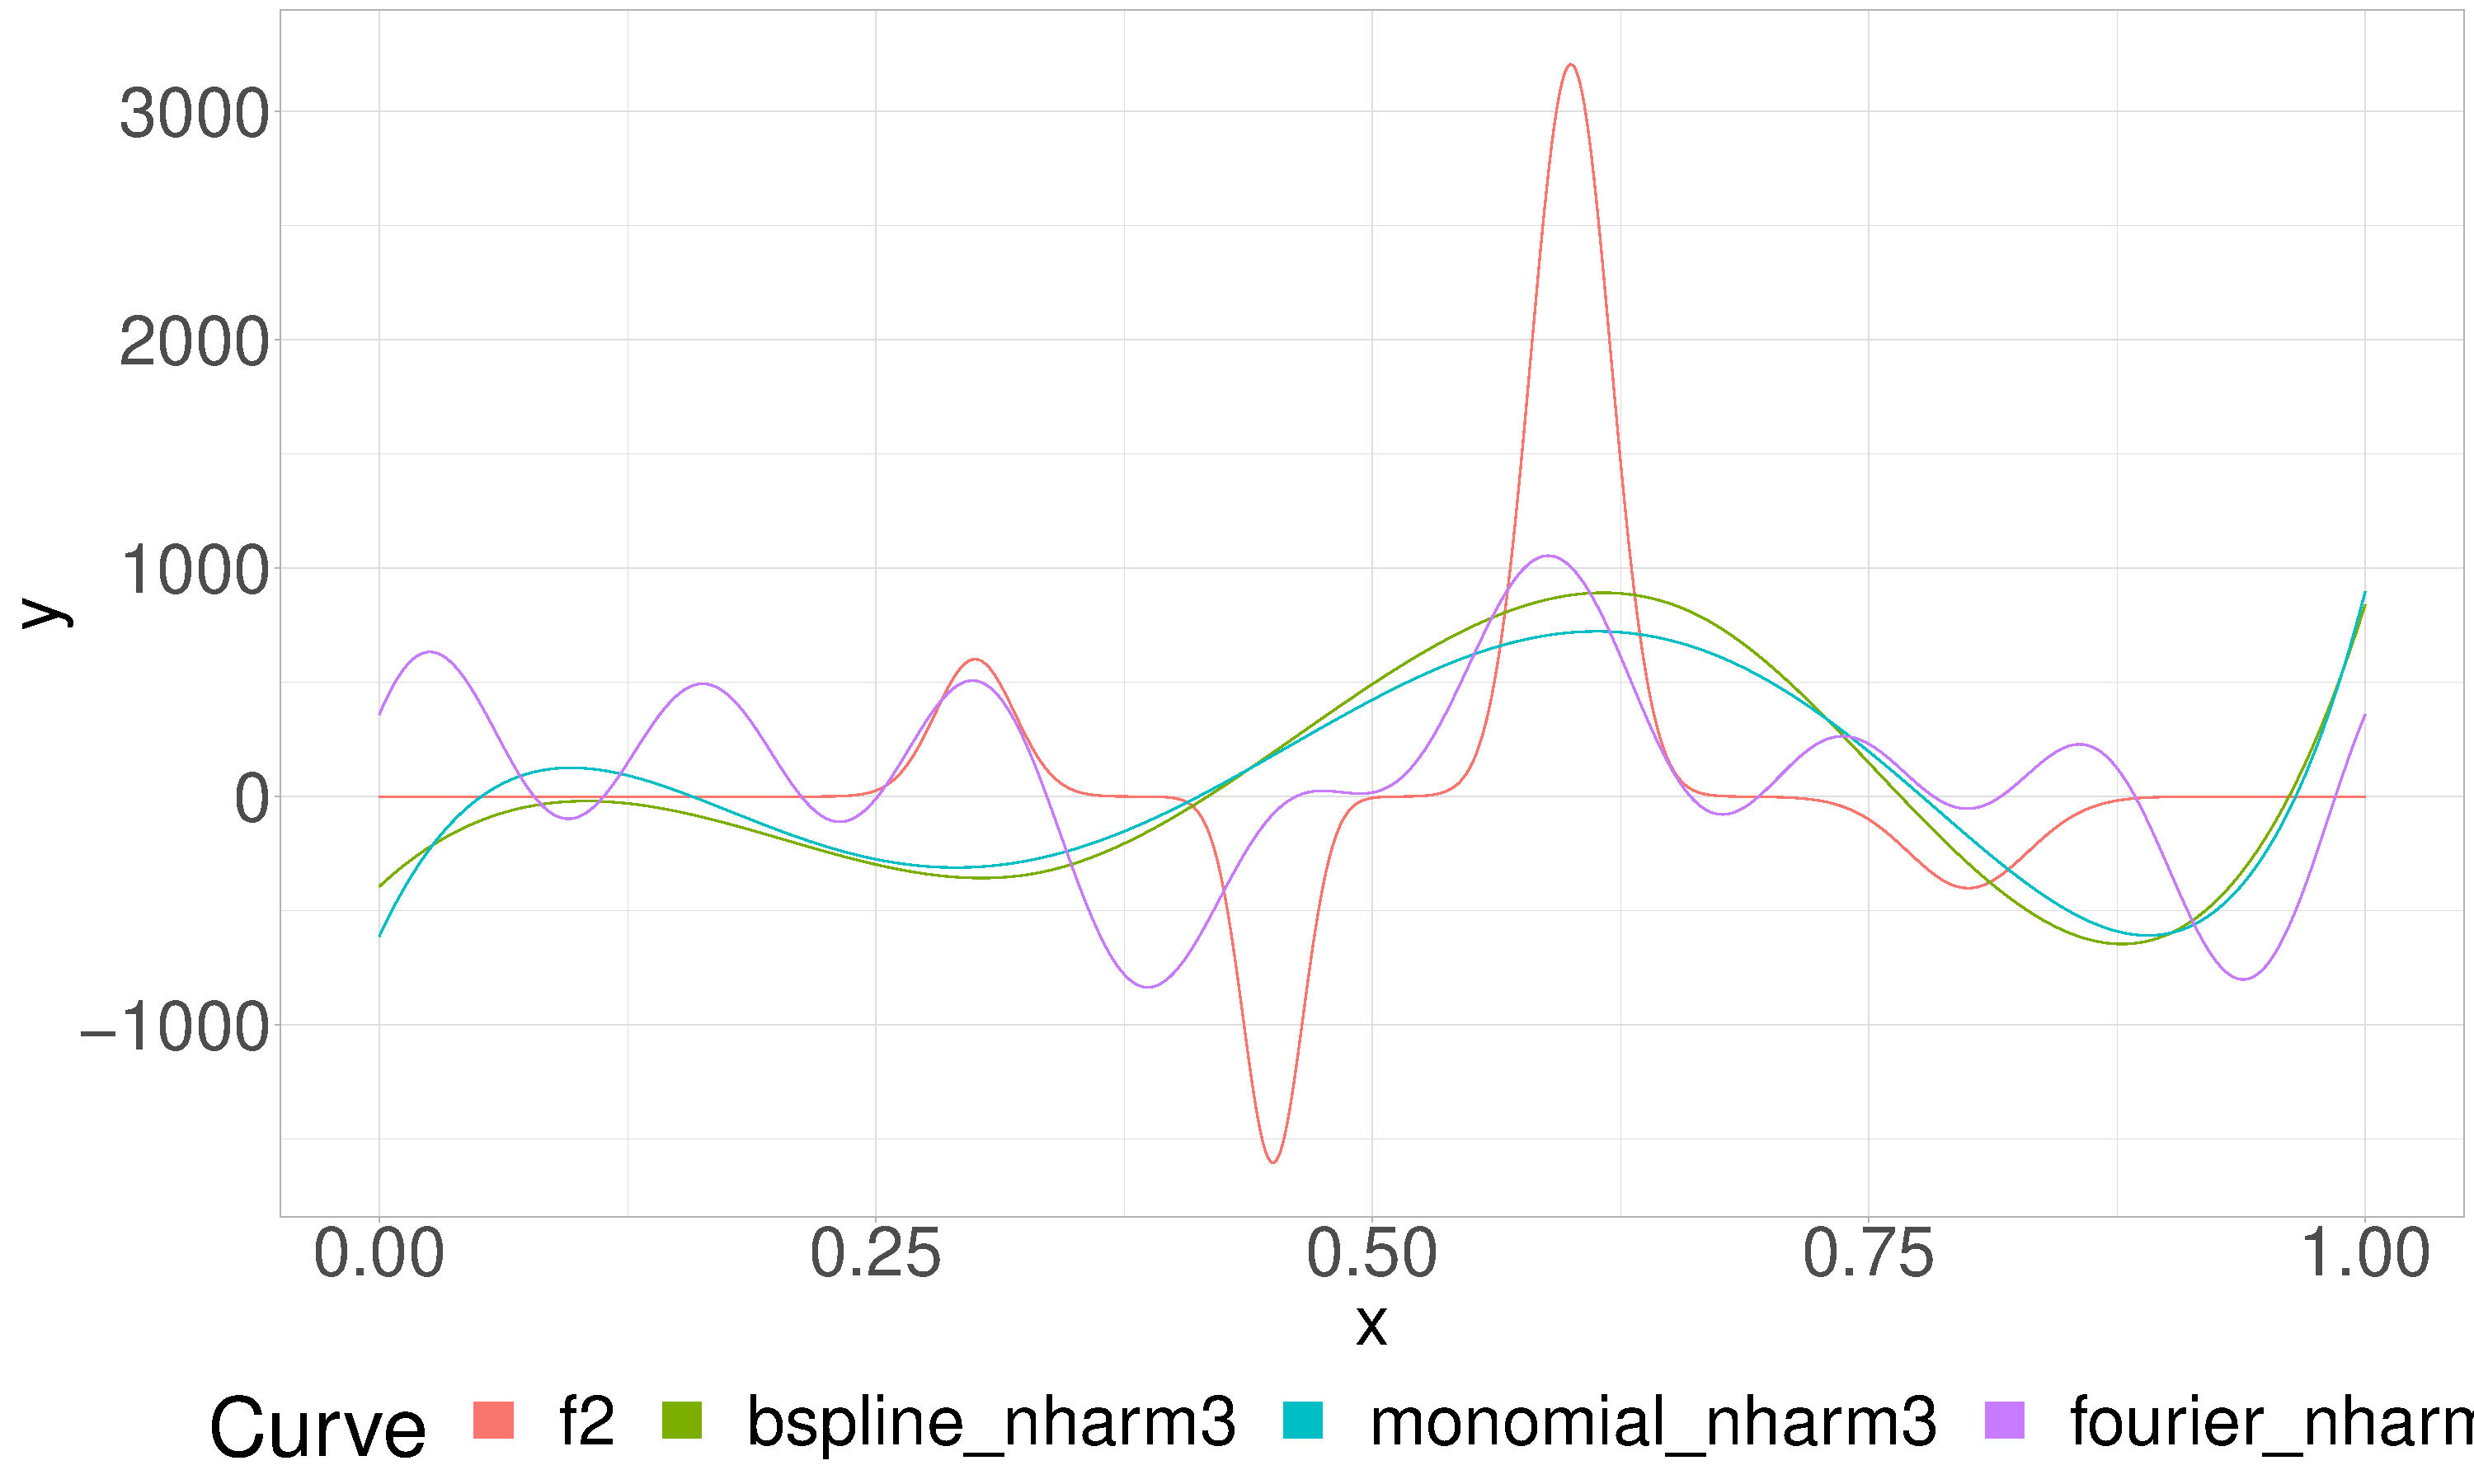
\includegraphics[width=\textwidth]{../Graphics/Curve\_Estimates/fpcr_nharm3_2_2.pdf}
			\caption{FPC Regression, 3 harmonics - $f_2, Y_2$}
			\label{fpcr_nharm3_2_2}
		\end{minipage}
	\end{figure}
	
	\begin{figure}[H]
		\centering
		\begin{minipage}{.5\textwidth}
			\centering
			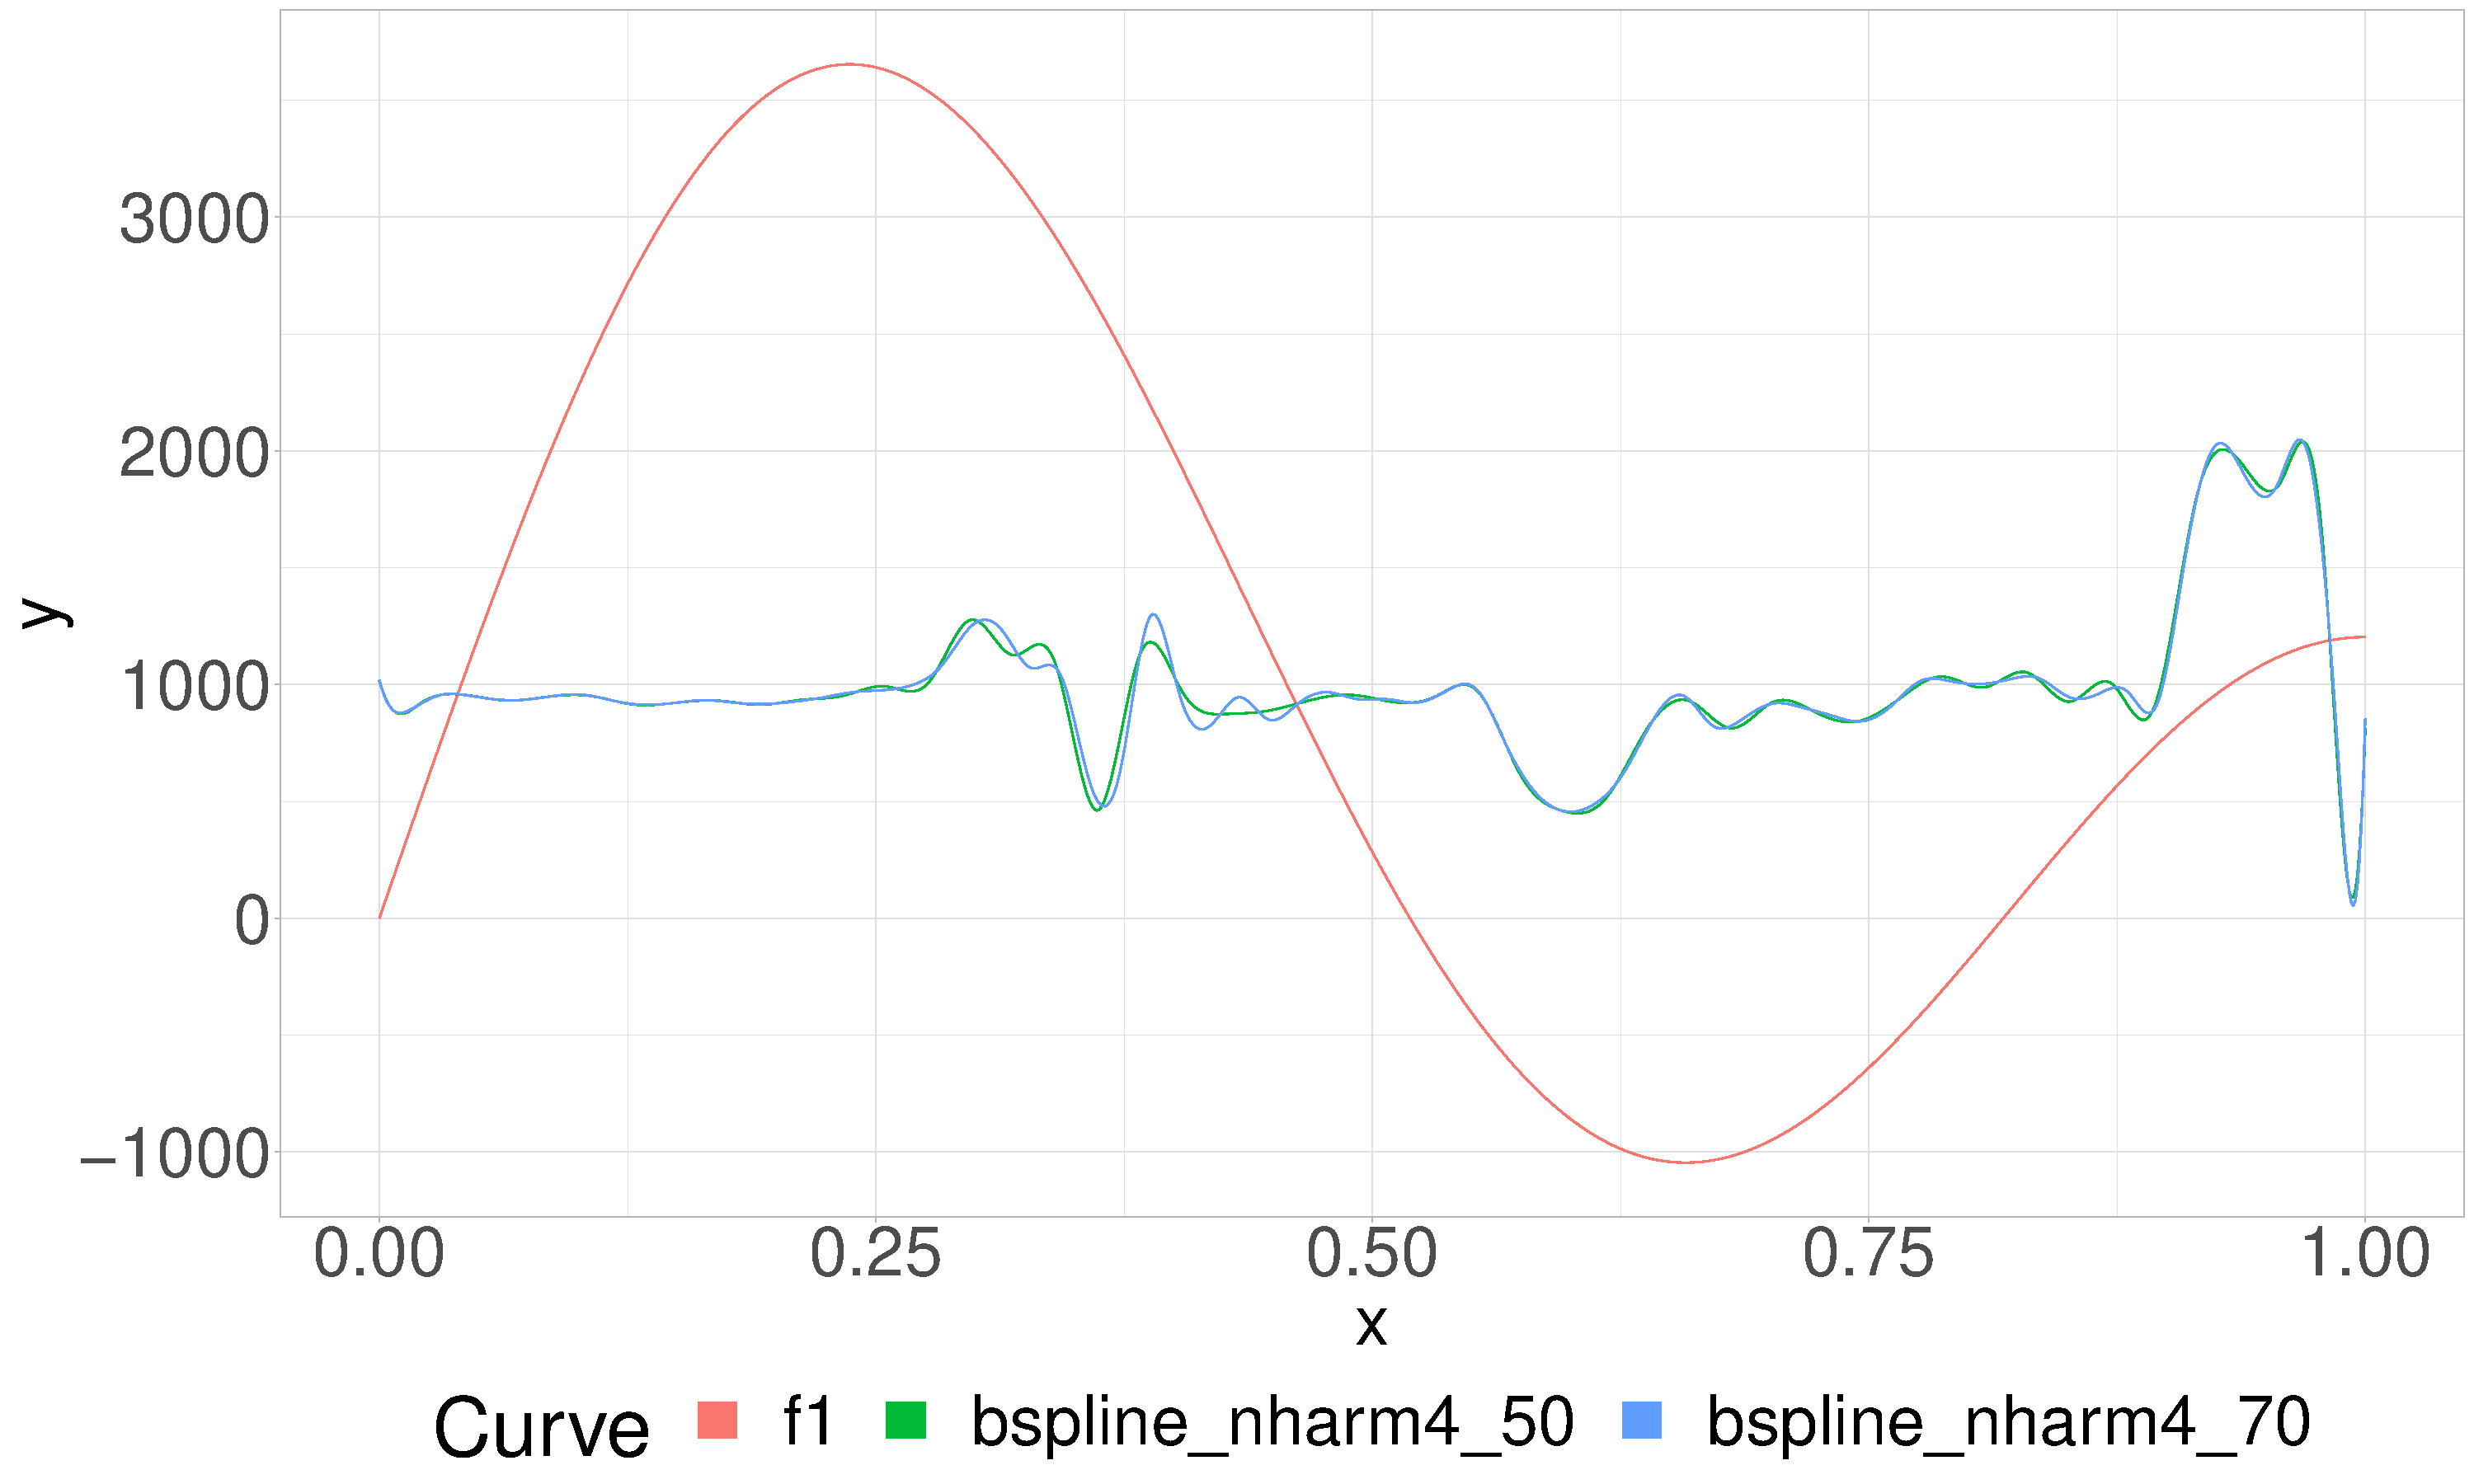
\includegraphics[width=\textwidth]{../Graphics/Curve\_Estimates/fpcr_nharm4_1_1.pdf}
			\caption{FPC Regression, 4 harmonics - $f_1, Y_1$}
			\label{fpcr_nharm4_1_1}
		\end{minipage}%
		\begin{minipage}{.5\textwidth}
			\centering
			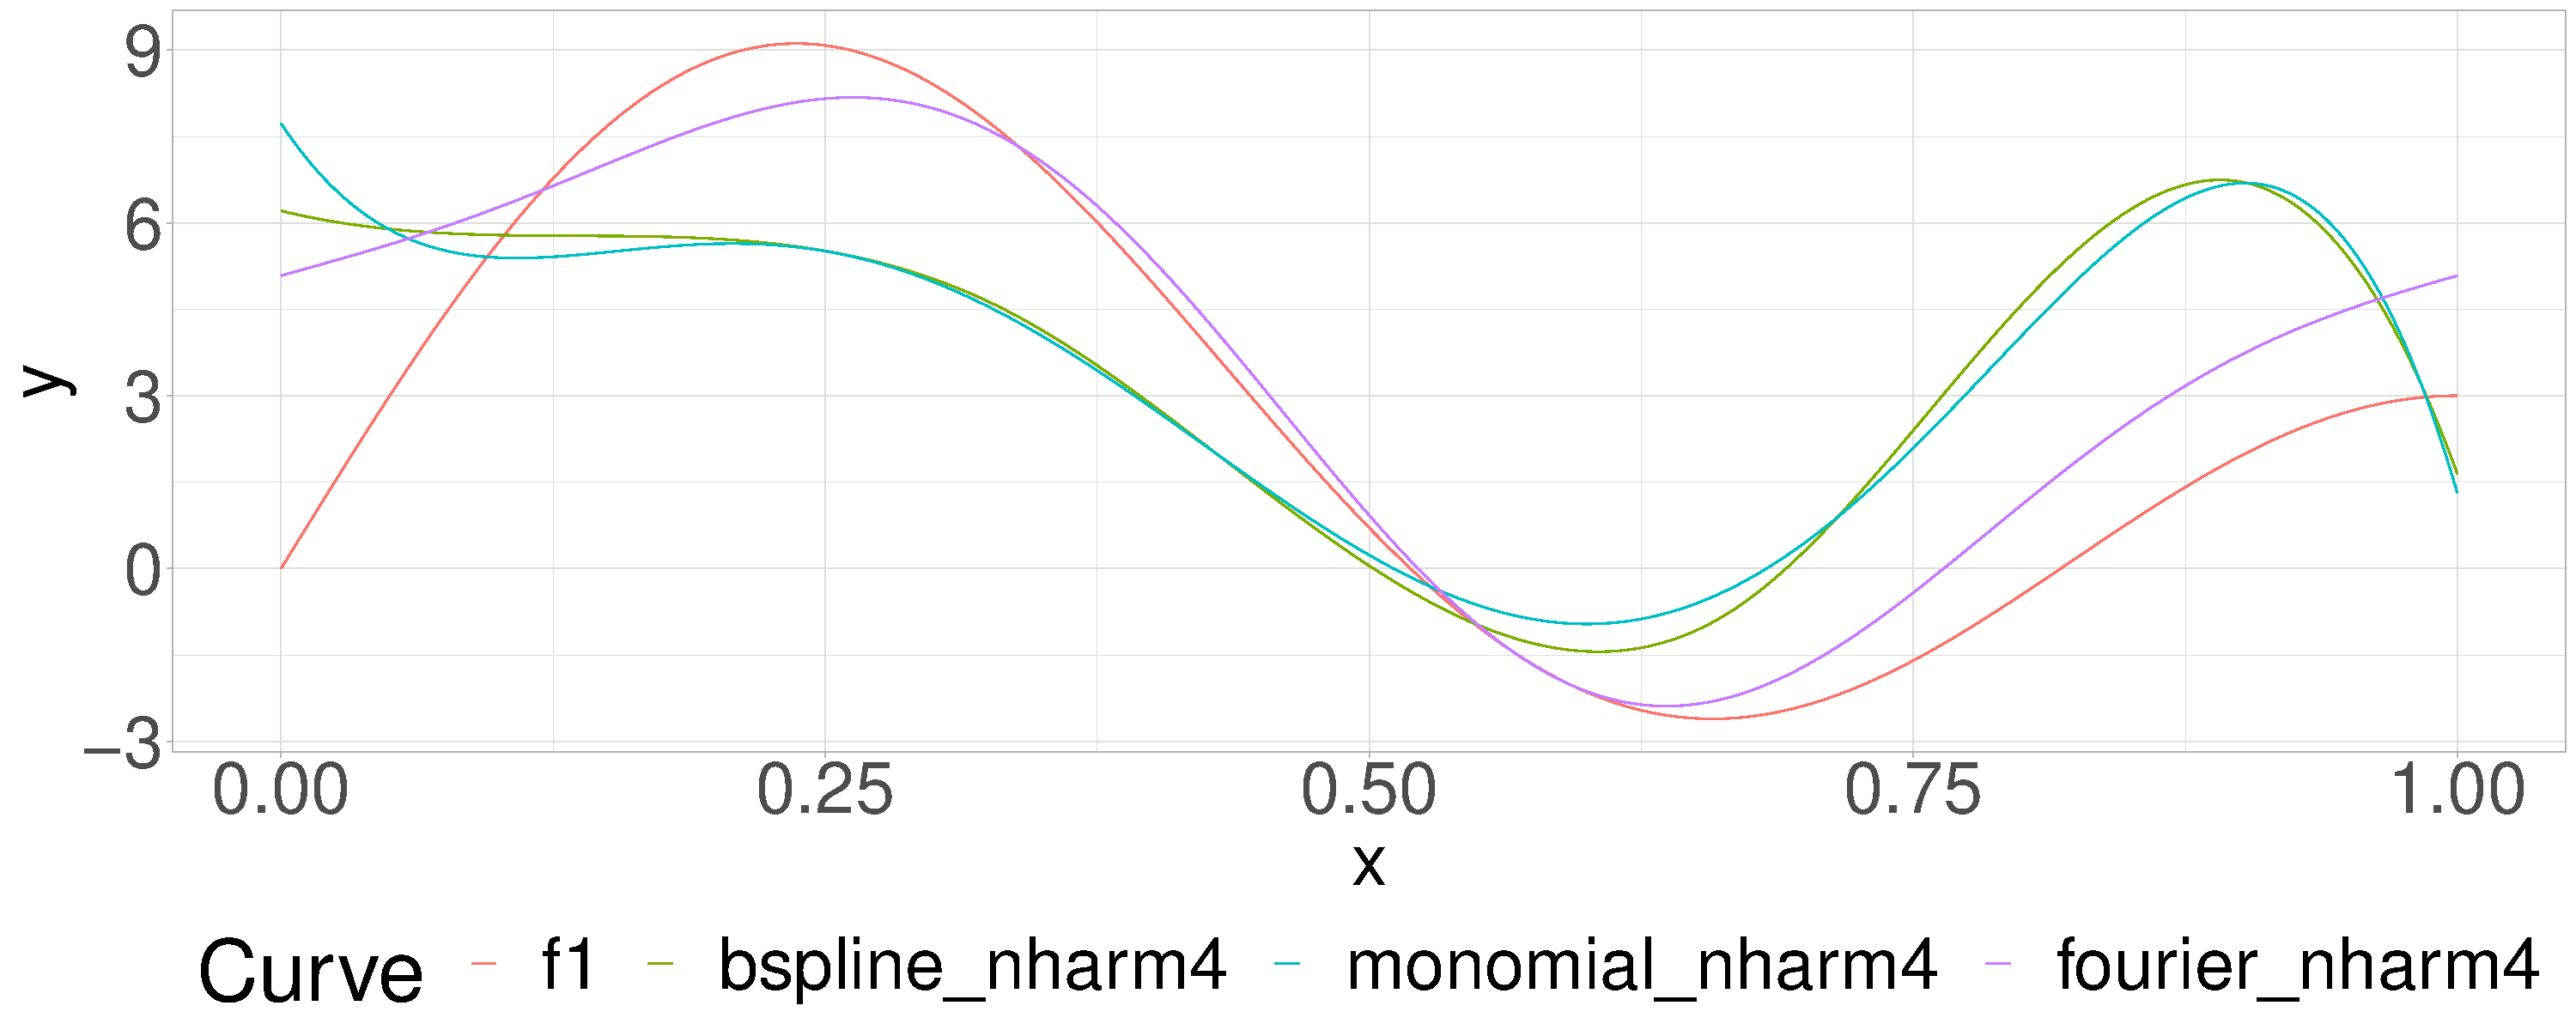
\includegraphics[width=\textwidth]{../Graphics/Curve\_Estimates/fpcr_nharm4_1_2.pdf}
			\caption{FPC Regression, 4 harmonics - $f_1, Y_2$}
			\label{fpcr_nharm4_1_2}
		\end{minipage}
	\end{figure}
	
	\begin{figure}[H]
		\centering
		\begin{minipage}{.5\textwidth}
			\centering
			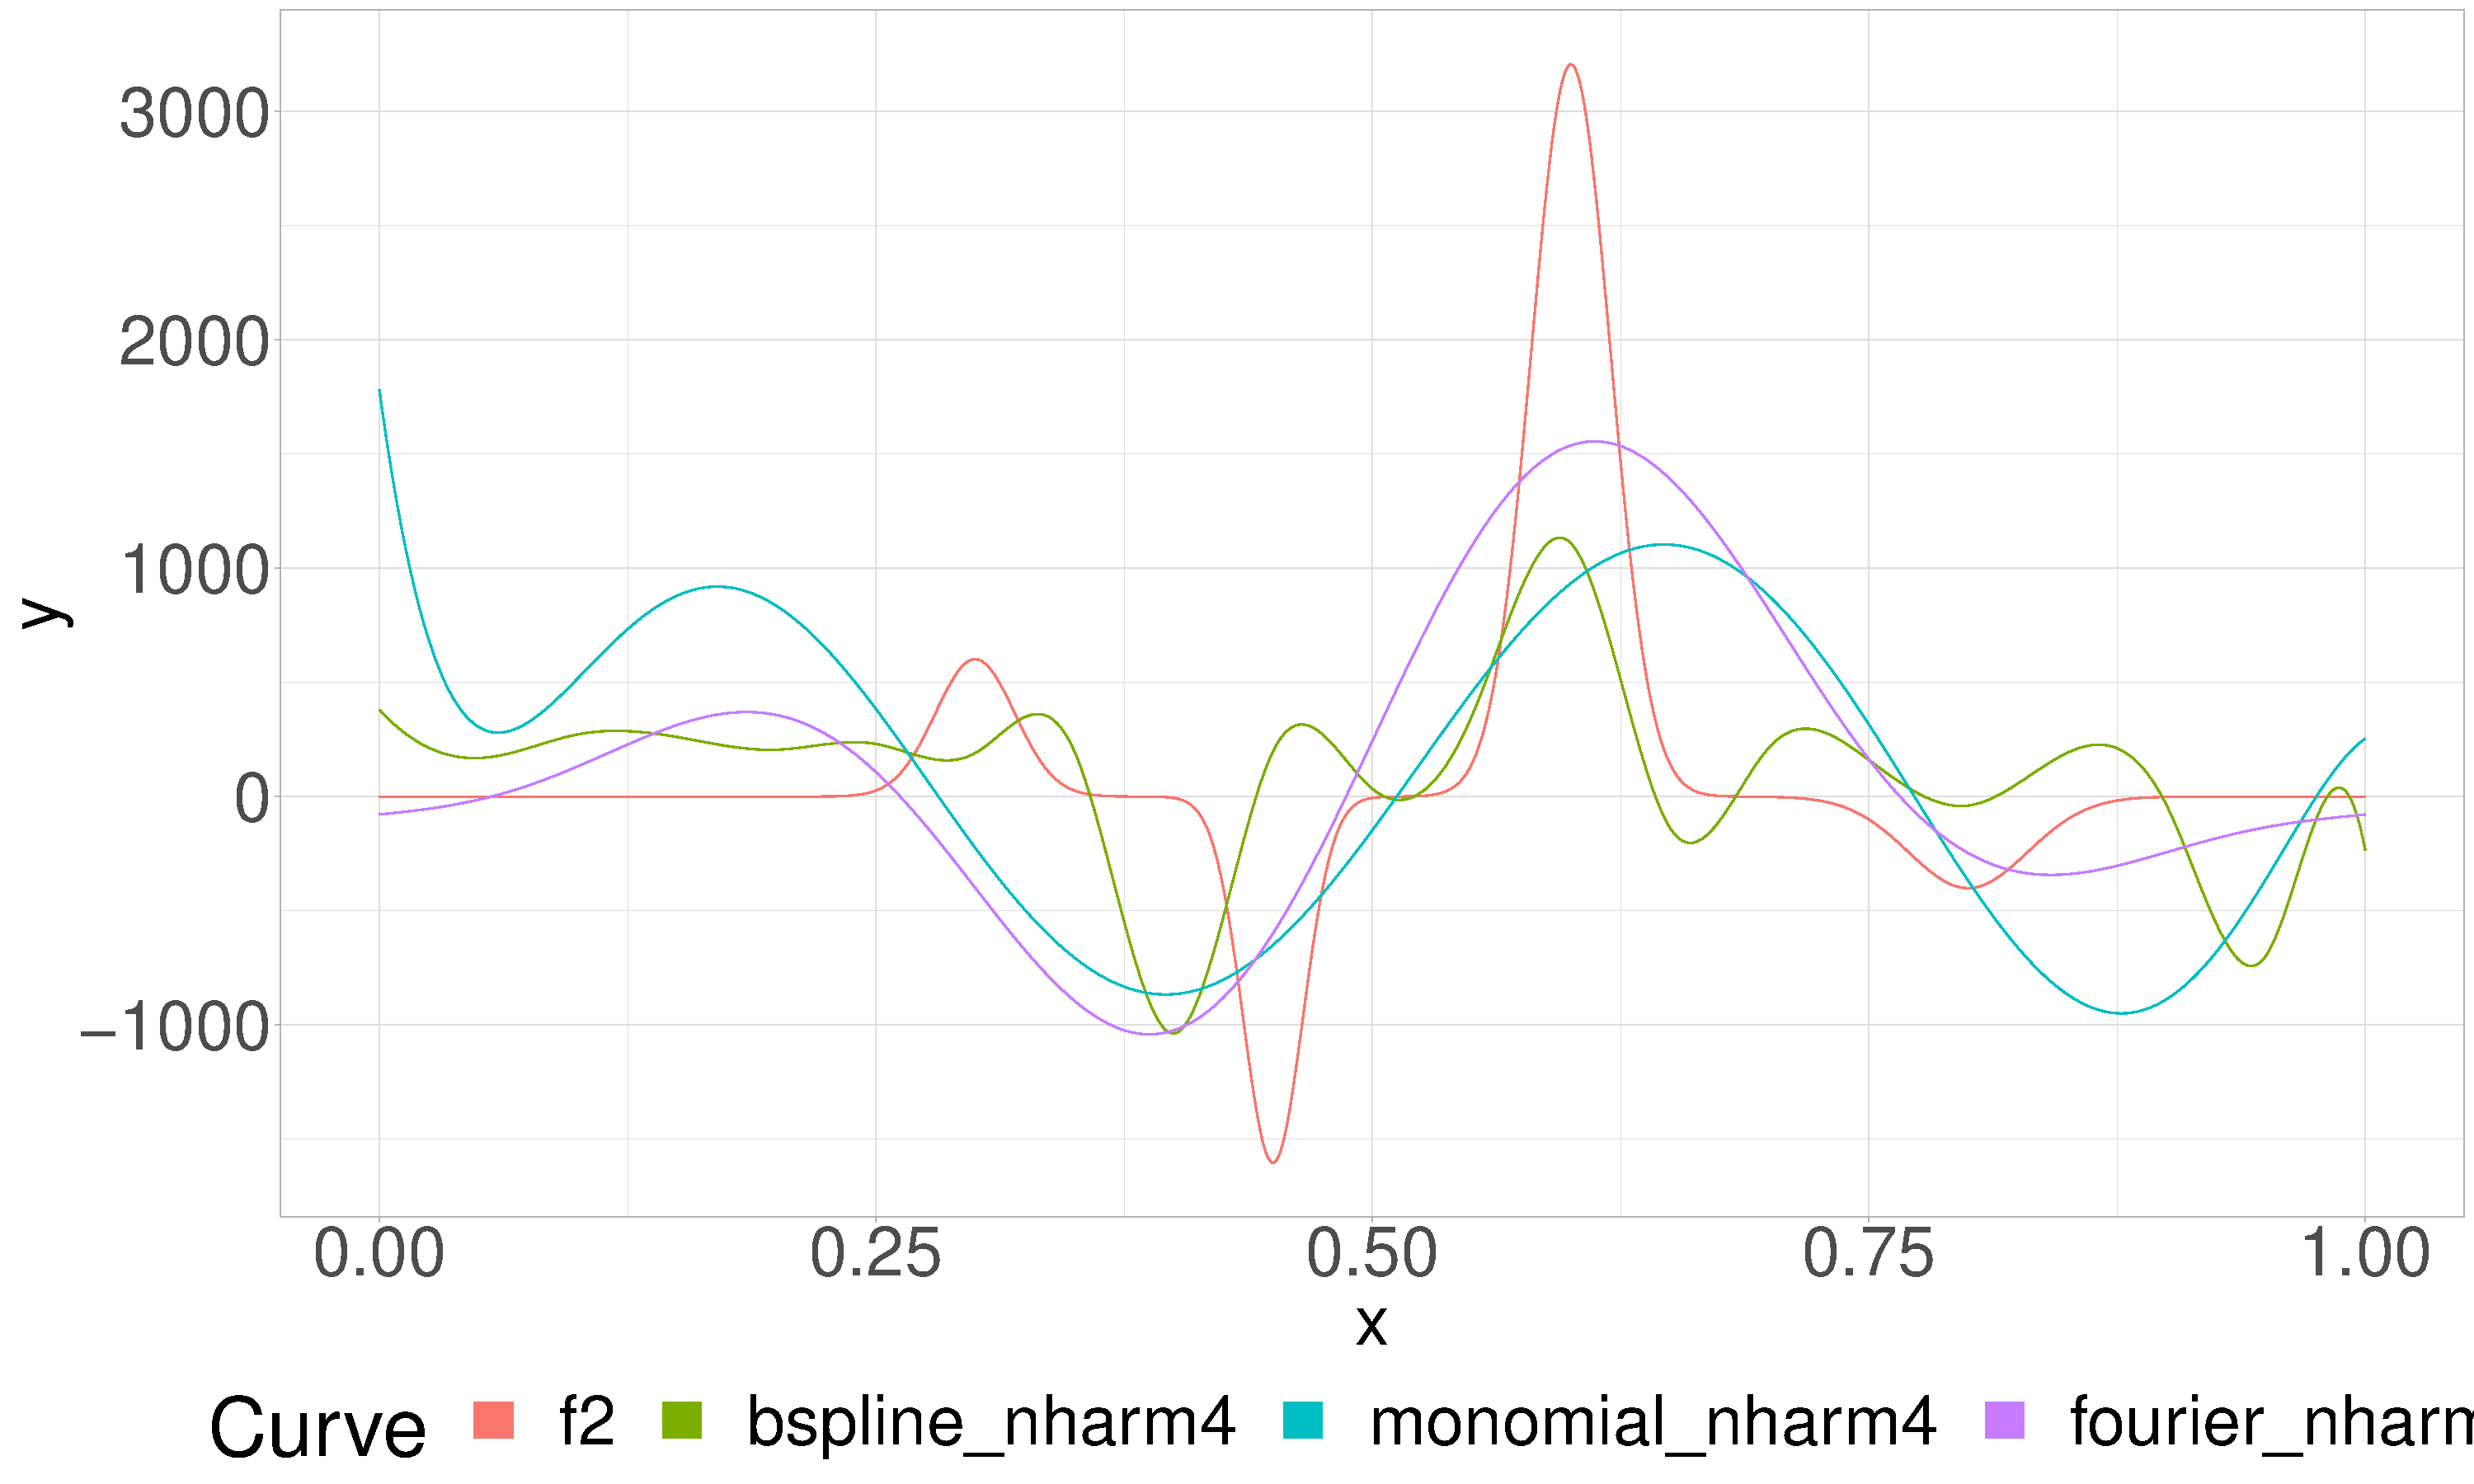
\includegraphics[width=\textwidth]{../Graphics/Curve\_Estimates/fpcr_nharm4_2_1.pdf}
			\caption{FPC Regression, 4 harmonics - $f_2, Y_1$}
			\label{fpcr_nharm4_2_1}
		\end{minipage}%
		\begin{minipage}{.5\textwidth}
			\centering
			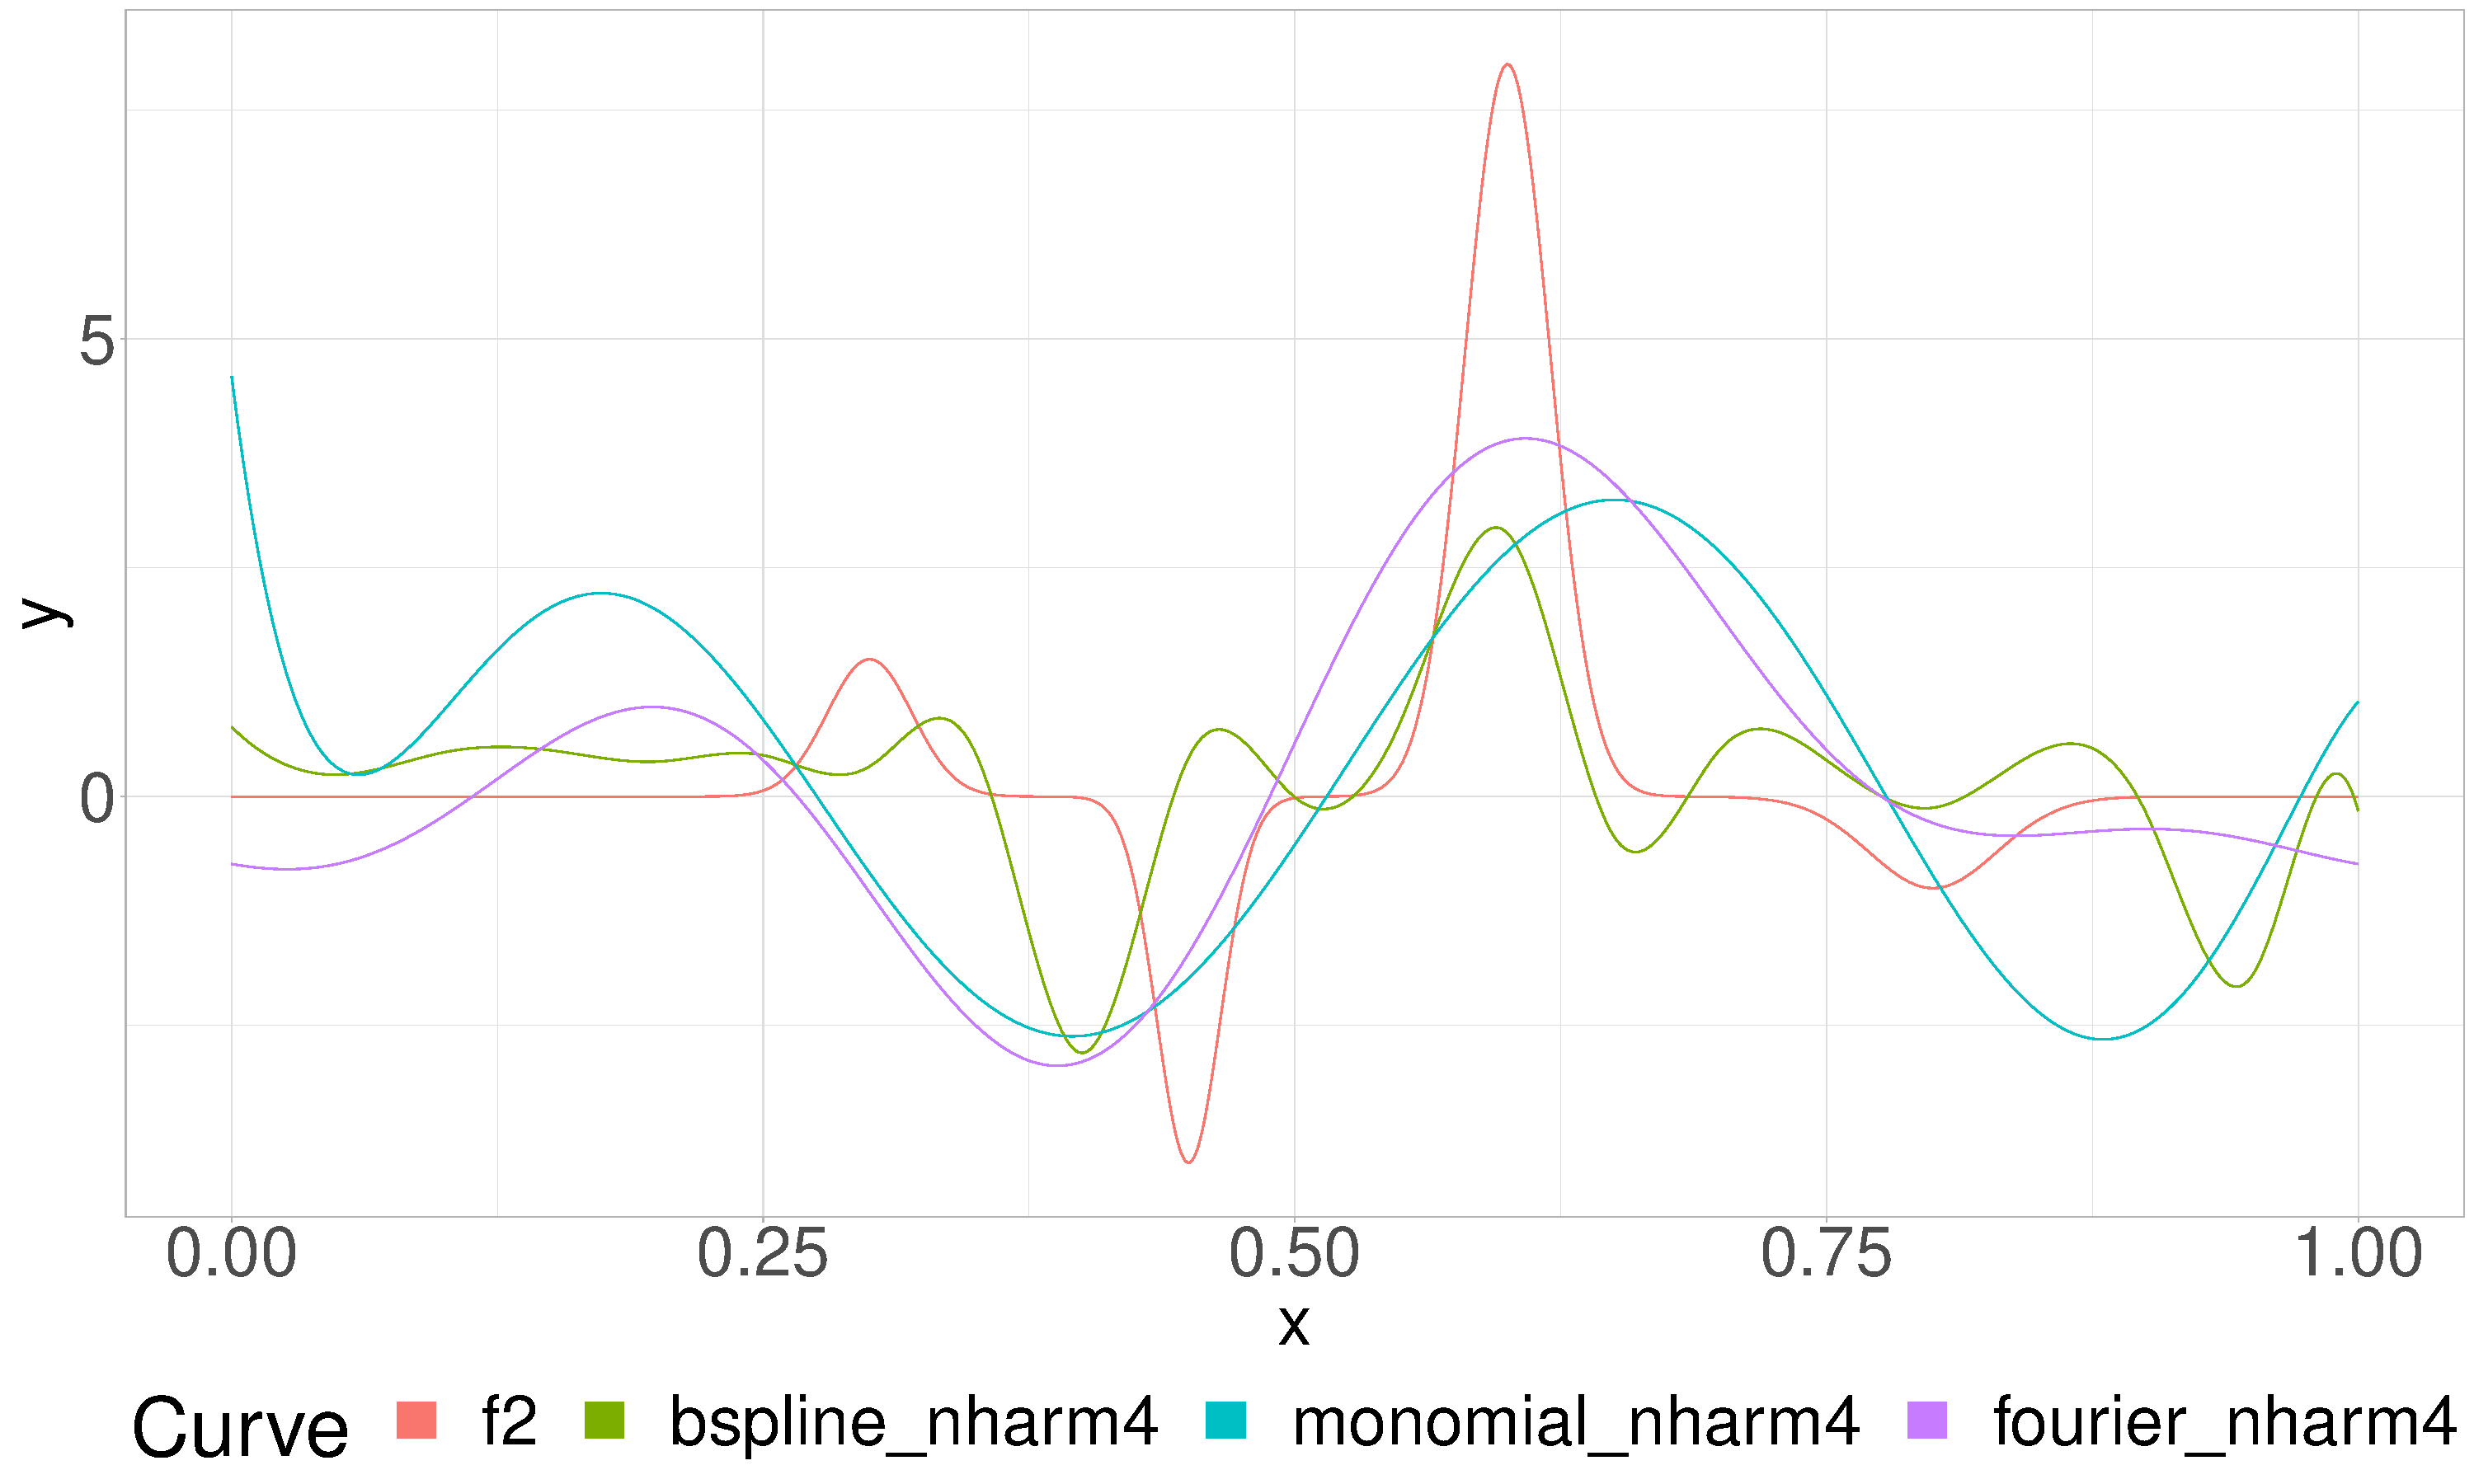
\includegraphics[width=\textwidth]{../Graphics/Curve\_Estimates/fpcr_nharm4_2_2.pdf}
			\caption{FPC Regression, 4 harmonics - $f_2, Y_2$}
			\label{fpcr_nharm4_2_2}
		\end{minipage}
	\end{figure}

\newpage
% extrernal file for all tables Tables


\subsection{Application Results}\label{Tables_appl}
The following results were rounded to 5 decimal places.
%%%%%%%%%%%%%%%%%%%%%%%%%%%%%%%%%%%%%%%%%%%
%\begin{table}[H]
%			\centering
%			\caption{Best Model Tabel - tmp}
%				\begin{tabular}{lllllll}
%					\cline{1-5}
%					 \boldmath{$f_1, Y_1$}                 & \boldmath{$f_1, Y_2$}                  & \boldmath{$f_2, Y_1$}                    & \boldmath{$f_2, Y_2$}               & \textbf{model} &  \\ \cline{1-5}
%5     & 3     & 5     & 5     & monomial basis  \\
%5     & 4     & 11    & 6     & bspline basis   \\
%5     & 3     & 9     & 7     & fourier basis   \\
%4     & 4     & 10    & 10    & monomial fpcr 2 \\
%5     & 5     & 6     & 6     & monomial fpcr 3 \\
%6     & 6     & 8     & 8     & monomial fpcr 4 \\
%5     & 5     & 4     & 4     & bspline fpcr 2  \\
%5     & 5     & 6     & 6     & bspline fpcr 3  \\
%6     & 6     & 23    & 23    & bspline fpcr 4  \\
%3     & 3     & 5     & 5     & fourier fcpr 2  \\
%3     & 3     & 15    & 15    & fourier fpcr 3  \\
%5     & 5     & 7     & 7     & fourier fpcr 4 
%\end{tabular}
%\end{table}

%\vspace{0.5cm}	
	
	%%%%%%%%%%%%%%%%%%%%%%%%%%%%%%%%%%%%%%%
	
	


	\begin{table}[H]
			\centering
			\caption{Application Results Basis Expansion Regression}
				\begin{tabular}{lll|lll}
\hline
\textbf{Monomial} & \textbf{B-Spline} & \textbf{Fourier}                      & \textbf{n\_basis} & \textbf{fold\_size} & \textbf{n\_folds} \\ \hline
2.29641  &          & \multicolumn{1}{l|}{}        & 2       & 5         & 12      \\
2.11258  &          & \multicolumn{1}{l|}{2.07767} & 3       & 5         & 12      \\
0.73444  & 0.73444  & \multicolumn{1}{l|}{}        & 4       & 5         & 12      \\
{\color[HTML]{FE0000} 0.24181}  & 0.2544   & \multicolumn{1}{l|}{0.07430} & 5       & 5         & 12      \\
8.88013  & 0.08621  & \multicolumn{1}{l|}{}        & 6       & 5         & 12      \\
         & 0.11177  & \multicolumn{1}{l|}{0.05021} & 7       & 5         & 12      \\
         & 0.05012  & \multicolumn{1}{l|}{}        & 8       & 5         & 12      \\
         & 0.07465  & \multicolumn{1}{l|}{{\color[HTML]{FE0000} 0.04808}} & 9       & 5         & 12      \\
         & {\color[HTML]{FE0000} 0.04574}  & \multicolumn{1}{l|}{}        & 10      & 5         & 12      \\
         & 0.05629  & \multicolumn{1}{l|}{0.05456} & 11      & 5         & 12      \\
         & 0.05291  & \multicolumn{1}{l|}{}        & 12      & 5         & 12      \\
         & 0.06083  & \multicolumn{1}{l|}{0.05558} & 13      & 5         & 12      \\
         & 0.06926  & \multicolumn{1}{l|}{}        & 14      & 5         & 12      \\
         & 0.09058  & \multicolumn{1}{l|}{0.07920} & 15      & 5         & 12      \\
         &          & \multicolumn{1}{l|}{}        & 16      & 5         & 12      \\
         &          & \multicolumn{1}{l|}{0.06161} & 17      & 5         & 12      \\
         &          & \multicolumn{1}{l|}{}        & 18      & 5         & 12      \\
         &          & \multicolumn{1}{l|}{0.10976} & 19      & 5         & 12      \\ 
\end{tabular}
\end{table}

\vspace{0.5cm}



	\begin{table}[H]
			\centering
			\caption{Application Results Monomial FPCR}
				\begin{tabular}{lll|lll}
\hline
\textbf{2 FPC} & \textbf{3 FPC} & \textbf{4 FPC}                      & \textbf{n\_basis} & \textbf{fold\_size} & \textbf{n\_folds} \\ \hline
2.29642                        &                                &                                & 2       & 5         & 12      \\
{\color[HTML]{FE0000} 2.17648} & 2.11259                        &                                & 3       & 5         & 12      \\
2.21978                        & 2.17702                        & 0.73432                        & 4       & 5         & 12      \\
2.21854                        & 2.23061                        & 2.35328                        & 5       & 5         & 12      \\
2.21896                        & {\color[HTML]{FE0000} 1.98803} & 0.84386                        & 6       & 5         & 12      \\
2.23156                        & 2.07872                        & 0.85358                        & 7       & 5         & 12      \\
2.19982                        & 2.25104                        & 0.11363                        & 8       & 5         & 12      \\
2.24343                        & 2.21964                        & 0.11476                        & 9       & 5         & 12      \\
2.18792                        & 2.11694                        & 0.12084                        & 10      & 5         & 12      \\
2.20919                        & 2.15677                        & {\color[HTML]{FE0000} 0.08986} & 11      & 5         & 12      \\
2.27197                        & 2.21142                        & 0.14176                        & 12      & 5         & 12  \\    
\end{tabular}
\end{table}

\vspace{0.5cm}



\begin{table}[H]
			\centering
			\caption{Application Results B-spline FPCR}
				\begin{tabular}{lll|lll}
\hline
\textbf{2 FPC} & \textbf{3 FPC} & \textbf{4 FPC}                        & \textbf{n\_basis} & \textbf{fold\_size} & \textbf{n\_folds} \\ \hline
2.24364                        & 2.1                            & 0.73432                       & 4       & 5         & 12      \\
2.21916                        & 2.21024                        & 2.35745                       & 5       & 5         & 12      \\
2.2088                         & 1.92703                        & 0.55305                       & 6       & 5         & 12      \\
2.22042                        & 2.10322                        & 1.03165                       & 7       & 5         & 12      \\
2.17938                        & 2.24933                        & 0.076                         & 8       & 5         & 12      \\
2.20726                        & 2.20003                        & 0.18801                       & 9       & 5         & 12      \\
2.23642                        & 2.08957                        & 0.05669                       & 10      & 5         & 12      \\
2.23069                        & 2.13131                        & 0.09795                       & 11      & 5         & 12      \\
2.22878                        & 2.14135                        & 0.05523                       & 12      & 5         & 12      \\
2.1994                         & 2.13177                        & 0.06089                       & 13      & 5         & 12      \\
2.20168                        & 2.14603                        & 0.07197                       & 14      & 5         & 12      \\
2.20372                        & 2.14908                        & 0.05159                       & 15      & 5         & 12      \\
2.16851                        & 2.13255                        & 0.05724                       & 16      & 5         & 12      \\
2.17341                        & 2.12780                        & 0.06545                       & 17      & 5         & 12      \\
2.18263                        & 2.00428                        & 0.05399                       & 18      & 5         & 12      \\
{\color[HTML]{FE0000} 2.15647} & 2.05871                        & 0.06774                       & 19      & 5         & 12      \\
2.19268                        & 1.96472                        & 0.05542                       & 20      & 5         & 12      \\
2.17718                        & 1.95345                        & 0.0595                        & 21      & 5         & 12      \\
2.1798                         & 1.99118                        & 0.05519                       & 22      & 5         & 12      \\
2.1966                         & {\color[HTML]{FE0000} 1.90692} & 0.05318                       & 23      & 5         & 12      \\
2.1786                         & 1.97124                        & 0.05725                       & 24      & 5         & 12      \\
2.18768                        & 1.95758                        & {\color[HTML]{FE0000} 0.0508} & 25      & 5         & 12      \\
\end{tabular}
\end{table}

\vspace{0.5cm}



\begin{table}[H]
			\centering
			\caption{Application Results Fourier FPCR}
				\begin{tabular}{lll|lll}
\hline
\textbf{2 FPC} & \textbf{3 FPC} & \textbf{4 FPC}                       & \textbf{n\_basis} & \textbf{fold\_size} & \textbf{n\_folds} \\ \hline
{\color[HTML]{FE0000} 2.13234} & 2.07788                        &                               & 3       & 5         & 12      \\
2.26267                        & 0.21409                        & 0.19585                       & 5       & 5         & 12      \\
2.15572                        & 0.06414                        & {\color[HTML]{FE0000} 0.0435} & 7       & 5         & 12      \\
2.16344                        & {\color[HTML]{FE0000} 0.05448} & 0.05256                       & 9       & 5         & 12      \\
2.16087                        & 0.06795                        & 0.05276                       & 11      & 5         & 12      \\
2.13984                        & 0.05848                        & 0.05154                       & 13      & 5         & 12      \\
2.17941                        & 0.14014                        & 0.06486                       & 15      & 5         & 12      \\
2.16465                        & 0.28983                        & 0.05143                       & 17      & 5         & 12      \\
2.18426                        & 0.43575                        & 0.05255                       & 19      & 5         & 12  	\\  
\end{tabular}
\end{table}

\vspace{0.5cm}




	\newpage
	
	\subsection{Application - Coefficient Function Estimates}\label{Estimates_Appl}
	\begin{figure}[H]
		\centering
		\begin{minipage}{.5\textwidth}
			\centering
			\includegraphics[width=\textwidth]{../Graphics/Appl\_Curve\_Estimates/appl\_basis\_expansion.pdf}
			\caption{Basis Expansion Regression}
			\label{basis_expansion_estimate_appl}
		\end{minipage}%
		\begin{minipage}{.5\textwidth}
			\centering
			\includegraphics[width=\textwidth]{../Graphics/Appl\_Curve\_Estimates/fpcr\_nharm2.pdf}
			\caption{2 Functional Principal Components}
			\label{FPCR2_estimate_appl}			
		\end{minipage}
	\end{figure}
	
	\begin{figure}[H]
		\centering
		\begin{minipage}{.5\textwidth}
			\centering
			\includegraphics[width=\textwidth]{../Graphics/Appl\_Curve\_Estimates/fpcr\_nharm3.pdf}
			\caption{3 Functional Principal Components}
			\label{FPCR3_estimate_appl}	
		\end{minipage}%
		\begin{minipage}{.5\textwidth}
			\centering
			\includegraphics[width=\textwidth]{../Graphics/Appl\_Curve\_Estimates/fpcr\_nharm4.pdf}
			\caption{4 Functional Principal Components}
			\label{FPCR4_estimate_appl}	
		\end{minipage}
	\end{figure}
	
	\section{Definitions and Proofs}
	\cite{alexanderian_KLexpansion_2015} was referred for the following definitions and proofs.
	
	\subsection{Definition (Hilbert-Schmidt Integral Operator)}\label{def_HS}
	Given a bounded domain $\mathcal{A} \subset \mathbb{R}^n$, we call a function $c : \mathcal{A} \times \mathcal{A} \rightarrow \mathbb{R}$ a Hilbert-Schmidt kernel if
	\begin{equation}
		\int_{\mathcal{A}} \int_{\mathcal{A}} \vert c(x,y) \vert ^2 dx dy < \infty
	\end{equation}
	where $c \in \mathbb{L}^2(\mathcal{A} \times \mathcal{A})$. Let $K$ be an integral operator on $\mathbb{L}^2(\mathcal{A})$ such that $K : \nu \rightarrow K \nu$ for $\nu \in \mathbb{L}^2(\mathcal{A})$, by
	
	\begin{equation}
		[K\nu](x) = \int_{\mathcal{A}} c(x,y) \nu(y) dy
	\end{equation}
	When an integral operator $K$ is linear and bounded, it is called a Hilbert-Schmidt operator. The linearity of the operator $K$ is simply proved. Additionaly assume that $\alpha, \beta \in \mathbb{R}$ and $\theta \in \mathbb{L}^2(\mathcal{A})$.
	\begin{equation}
		\begin{split}
			[K (\alpha \nu + \beta \theta)](x) =& \int_{\mathcal{A}} c(x,y)(\alpha \nu(y) + \beta \theta(y)) dy\\
			= & \int_{\mathcal{A}} c(x,y) \alpha \nu(y) dy + \int_{\mathcal{A}} c(x,y) \beta \theta(y) dy\\
			= & \alpha\int_{\mathcal{A}} c(x,y) \nu (y) dy + \beta\int_{\mathcal{A}} c(x,y) \theta (y) dy\\
			= & \alpha[K\nu](x) + \beta[K\theta](x)
		\end{split}
	\end{equation}
	For boundedness of the oprator $K$,
	\begin{equation}
		\begin{split}
			\Vert K\nu \Vert^{2}_{\mathbb{L}^2(\mathcal{A})} = & \int_{\mathcal{A}} \biggl\vert [K\nu](x) \biggr\vert^2 dx\\
			= &\int_{\mathcal{A}} \biggl\vert \int_{\mathcal{A}}c(x,y)\nu(y)dy \biggr\vert^2dx\\
			\leq & \int_{\mathcal{A}}\biggl(\int_{\mathcal{A}}\vert c(x,y) \vert^2dy\biggr) \biggl(\int_{\mathcal{A}}\vert \nu(y) \vert ^2 dy \biggr)dx \quad \text{(Cauchy-Schwarz)}\\
			= & \Vert c \Vert_{\mathbb{L}^2(\mathcal{A} \times \mathcal{A})}\Vert \nu \Vert_{\mathbb{L}^2} < \infty
		\end{split}
	\end{equation}
	
	\subsection{Lemma} \label{Proof1}
	The curves $X(t) \in \mathbb{L}^2[0,1]$ is expanded by the Eigenfunctions $\{\nu^m\}$ as Equation \ref{KarhunenLoeve}. The coefficients $\xi^{m}$ corresponding to Eigenfunctions $\nu^m$ satisfy the following properties:
	
	\begin{multicols}{2}
		\begin{enumerate}
			\item $\mathbb{E}\left[\xi^m(\omega)\right] = 0$
			\item $Cov\left(\xi^m(\omega), \xi^n(\omega)\right) = \delta^{m,n}\lambda^m$% if $m \neq n$
			\item $Var\left(\xi^m(\omega)\right) = \lambda^m$
		\end{enumerate}
	\end{multicols}

	Remind that $\delta^{m,n} = 0$ if $m \neq n$, otherwise 1.
	
	\begin{proof}
		Assume that $F(t)$ is the centered process of $X(t)$, namely, $F(t) = X(t) - \int_{\Omega}X(t)dP(\omega)$. To obtain the first result, we can show that
		
		\begin{equation}\label{Lemma1}
			\begin{split}
				\mathbb{E}[\xi^m] = & \mathbb{E} \biggl\lbrack \int_{0}^{1} F(t) \nu_{j}(t)dt\biggr\rbrack\\
				= & \int_{\Omega} \int_{0}^{1} F(t) \nu^m(t) dt dP(\omega)\\
				= & \int_{0}^{1} \int_{\Omega} F(t) \nu^m(t) dP(\omega) dt \quad \text{(Fubini)}\\
				= & \int_{0}^{1} {\color{red}\int_{\Omega} F(t) dP(\omega)} \nu^m(t) dt\\
				= & \int_{0}^{1} {\color{red}\mathbb{E}[F(t)]} \nu^m(t) dt = 0
			\end{split}
		\end{equation}
	
		where $\mathbb{E}[F(t)]$ is 0 since $F(t)$ is a centered process.
		The second claim is proved as:
		
		\begin{equation}\label{Lemma2}
			\begin{split}
				\mathbb{E} [\xi^m \xi^n] = & \mathbb{E}  \biggl\lbrack \int_{0}^{1} F(s) \nu^m(s)ds \int_{0}^{1} F(t) \nu^n(t)dt  \biggr\rbrack\\
				= & \mathbb{E} \biggl\lbrack {\int_{0}^{1} \int_{0}^{1} F(s) \nu^m(s) F(t) \nu^n(t) ds dt} \biggr\rbrack \quad \text{(Fubini)}\\
				= & \int_{0}^{1} {\color{red}\int_{0}^{1} \mathbb{E}[{F(s)F(t)}] \nu^m(s)} \nu^n(t) {\color{red}ds} dt\\
				= & \int_{0}^{1} {\color{red}\left(\int_{0}^{1}c(s,t)\nu^m(s)ds \right)} \nu^n(t) dt \\
				= & \int_{0}^{1}{\color{red}[K\nu^m](t)}\nu^n(t)dt\\
				= & \langle K \nu^m, \nu^n \rangle\\
				= & \langle \lambda^m \nu^m, \nu^n \rangle = \delta^{m,n}\lambda^{m}
			\end{split}
		\end{equation}
	
		where $\delta^{m,n} = 1$ if $m = n$, otherwise 0. The result is produced from orthonormality of the Eigenfunctions.
		
		\begin{equation}
			Cov\left(\xi^m, \xi^n\right) = \mathbb{E}[\xi^m \xi^n] - \mathbb{E}[\xi^m]\mathbb{E}[\xi^n] = \delta^{m,n}\lambda^{m}
		\end{equation}
	
		where $\mathbb{E}[\xi^m] = \mathbb{E}[\xi^n] = 0$ as the first property.
		The last assertion is confirmed from the above two properties.
		
		\begin{equation}\label{Lemma3}
			Var[\xi^m] = \mathbb{E}\left[(\xi^m - \mathbb{E}[\xi^m])^{2}\right] = \mathbb{E}[(\xi^m)^{2}] =\lambda^m
		\end{equation}
	
		The original process $X(t)$ also has the same properties as the centered one since
		
		\begin{equation}
			X(t) = F(t) + \mathbb{E}[X(t)] = \mu(t) + \sum_{m=1}^{\infty}\xi^m\nu^m(t)
		\end{equation}
	
	\end{proof}
	
	
	\subsection{Theorem (Karhunen-Lo\'{e}ve expansion)} \label{Proof2}
	
	Let $X : [0,1]  \rightarrow \mathbb{R}$ be a mean-square continuous stochastic process, namely, $\lim\limits_{\epsilon \rightarrow 0} \mathbb{E}[(X(t+\epsilon) - X(t))^2]$ = 0, such that $X \in \mathbb{L}^{2}[0,1]$. Then there exists a basis ${\xi^m}$ of $\mathbb{L}^2[0,1]$ such that for all $t \in [0,1]$,
	
	\begin{equation}
		X(t) = \mu(t) + \sum_{m=1}^{\infty} \xi^m \nu^m(t),
	\end{equation}

	where $\mu(t)$ is the mean function of $X(t)$ and coefficients $\xi^m$ are given by $\int_{0}^{1} (X(t) - \mu(t)) \nu^m(t)dt$. These coefficients satisfy the following conditions.
	
	\begin{multicols}{2}
		\begin{enumerate}
			\item $\mathbb{E}\left[\xi^m(\omega)\right] = 0$
			\item $Cov\left(\xi^m(\omega), \xi^n(\omega)\right) = \delta^{m,n}\lambda^m$ %if $m \neq n$
			\item $Var\left(\xi^m(\omega)\right) = \lambda^m$
		\end{enumerate}
	\end{multicols}

	\begin{proof}
		
		Let $K$ be a Hilbert-Schmidt operator as in Equation \ref{HSKernal}.We know that $K$ has a complete set of Eigenfunctions ${\nu^m}$ in $\mathbb{L}^{2}[0,1]$  and non-negative Eigenvalues $\lambda^m$ since $K$ is a positive compact self-adjoint operator. With the reminder that $\xi^m$ satisfy the three conclusions by Lemma \ref{Proof1}, we prove this expansion by considering
		
		\begin{equation}
			\epsilon_{N}(t) := \mathbb{E} \left[\bigg( X(t) -\mu(t)- \sum_{m=1}^{N} \xi^m \nu^m(t)\bigg)^2 \right]
			= \mathbb{E} \left[\bigg( F(t) - \sum_{m=1}^{N} \xi^m \nu^m(t)\bigg)^2 \right]
		\end{equation}
	
		where $F(t)$ is the centered process of $X(t)$.
		Once it is shown that $\lim\limits_{N \rightarrow \infty} \epsilon_{N}(t) = 0$ uniformly in [0,1], the proof is completed.
		
		\begin{equation}\label{Thr1}
			\begin{split}
				\epsilon_{N}(t) = &\mathbb{E} \left[\bigg( F(t) - \sum_{m=1}^{N} \xi^m 	\nu^m(t)\bigg)^2 \right]\\
				= & \mathbb{E}[F(t)^{2}] - 2\mathbb{E}\bigg[F(t)\sum_{m=1}^{N}\xi^m\nu^m(t)\bigg] + \mathbb{E}\bigg[\sum_{m=1}^{N}\sum_{n=1}^{N}\xi^m\xi^n\nu^m(t)\nu^n(t)\bigg]
			\end{split}
		\end{equation}
		
		Here, $\mathbb{E}[F(t)^{2}] = c(t,t)$ as in Equation \ref{CovarianceFunction} since $F(t)$ is the centered process. Now, take the second term
		
		\begin{equation}\label{Thr2}
			\begin{split}
				\mathbb{E} \bigg[ F(t) \sum_{m=1}^{N} {\color{red}\xi^m}\nu^m(t) \bigg] = & \mathbb{E} \left[ F(t) \sum_{m=1}^{N} {\color{red}\bigg(\int_{0}^{1} F(s)\nu^m(s)ds\bigg)} \nu^m(t) \right]\\
				= & \mathbb{E} \left[ \sum_{m=1}^{N} \bigg(\int_{0}^{1} F(t)F(s)\nu^m(s)ds\bigg) \nu^m(t) \right]\\
				= & \sum_{m=1}^{N} \bigg(\int_{0}^{1} {\color{blue}\mathbb{E}[F(t)F(s)]}\nu^m(s)ds\bigg)\nu^m(t)\\
				= & \sum_{m=1}^{N} {\color{teal}\bigg(\int_{0}^{1} {\color{blue}c(t,s)} \nu^m(s)ds\bigg)}\nu^m(t)\\
				= & \sum_{m=1}^{N}{\color{teal}[K\nu^m](t)}\nu^m(t) \\
				= &\sum_{m=1}^{N}{\color{teal}\lambda^m\nu^m(t)}\nu^m(t) = \sum_{m=1}^{N}\lambda^m\nu^m(t)^{2}
			\end{split}
		\end{equation} 
		
		where the covariance function $c(t,s)$ has the Hilbert-Schmidt operator as in Equation \ref{HSKernal}. It turns out the product of the Eigenfunction and the corresponding Eigenvalue. For the last term, we derive from Equation \ref{Lemma2} that
		
		\begin{equation}\label{Thr3}
			\begin{split}
				\mathbb{E}\bigg[\sum_{m=1}^{N} \sum_{n=1}^{N} \xi^m \xi^n \nu^m(t) \nu^n(t)\bigg] = & \sum_{m=1}^{N} \sum_{n=1}^{N} \mathbb{E}[\xi^m \xi^n] \nu^m(t) \nu^n(t)\\
				= & \sum_{m=1}^{N} \sum_{n=1}^{N} \delta^{m,n} \lambda^m \nu^m(t) \nu^n(t) = 		\sum_{m=1}^{N} \lambda^m \nu^m(t)^{2}
			\end{split}	
		\end{equation}
	
		where $\delta_{m,n} = 1$ if $m=n$, otherwise 0. Therefore, by Equations \ref{Thr1}, \ref{Thr2}, and \ref{Thr3} we obtain
		
		\begin{equation}
			\epsilon_{N}(t) = c(t,t) - \sum_{m=1}^{N} \lambda^m \nu^m(t) \nu^m(t)
		\end{equation}
		
		implementing Mercer's Theorem this proof is concluded by
		
		\begin{equation}
			\lim\limits_{N \rightarrow \infty} \epsilon_{N}(t) = \lim\limits_{n \rightarrow \infty} \mathbb{E} \left[\bigg( F(t) - \sum_{m=1}^{N} \xi^m \nu^m(t)\bigg)^2 \right] = 0
		\end{equation}
	
	\end{proof}

	\newpage
	
	\section{Bibliography}
	\printbibliography[heading=none]	
	
	\newpage
	\section*{Affidavit}
	
	\vspace{2cm}
	"I hereby confirm that the work presented has been performed and
	interpreted solely by myself except for where I explicitly identified the
	contrary. I assure that this work has not been presented in any other
	form for the fulfillment of any other degree or qualification. Ideas
	taken from other works in letter and in spirit are identified in every
	single case."
	
	\vspace{2cm}
	Bonn, 11.02.2021 \hrulefill \\
	\hspace*{0mm}Jonghun Baek
	
	\vspace{2cm}
	Bonn, 11.02.2021 \hrulefill \\
	\hspace*{0mm}Jakob R. Juergens
	
	\vspace{2cm}
	Bonn, 11.02.2021 \hrulefill \\
	\hspace*{0mm}Jonathan Willnow
	
	
\end{document}